% --------------------------------------------------------------------

\chapter[Cosmology]{Accurate Cosmological Measurements on the Largest Scales}
\def\chpname{cosmo}\label{chp:\chpname}

Chapter editors:
\credit{egawiser},
\credit{MichelleLochner}.

Contributing authors:
\credit{HumnaAwan},
\credit{egawiser},
\credit{pkurczynski},
\credit{rhiannonlynne},
\credit{jmeyers314},
\credit{tonytyson},
\credit{MelissaGraham},
\credit{SamSchmidt},
\credit{connolly},
\credit{ivezic},
\credit{jhrlsst},
\credit{rbiswas4},
\credit{sethdigel},
\credit{astrofoley},
\credit{lgalbany},
\credit{pgris},
\credit{ReneeHlozek},
\credit{saurabhwjha},
\credit{RickKessler},
\credit{AlexGKim},
\credit{aimalz},
\credit{jasonmcewen},
\credit{janewman-pitt-edu},
\credit{hiranyapeiris},
\credit{kponder},
\credit{rlschuhmann},
\credit{astrostubbs},
\credit{wmwv},
\credit{drphilmarshall},
\credit{tanguita}

% \section*{Summary}
% \addcontentsline{toc}{section}{~~~~~~~~~Summary}
%
% Executive summary goes here, highlighting the primary conclusions from
% the chapter's science cases. This should be abstract length, no more:
% say, 200 words.

% --------------------------------------------------------------------

\section{Introduction}
\label{sec:\chpname:intro}

Cosmology is one of the key science themes for which LSST was
designed. Our goal is to measure cosmological parameters, such as the
equation of state of dark energy or departures from General
Relativity, with sufficient accuracy to distinguish one model from
another and hence drive our theoretical understanding of how the
universe works as a whole. To do this will necessarily involve a
variety of different measurements that can act as cross-checks and break
any parameter degeneracies.

The  Dark Energy Science Collaboration (DESC) has identified five
different cosmological probes enabled by the LSST: weak lensing (WL),
large-scale structure (LSS), Type Ia supernovae (SN), strong lensing
(SL), and clusters of galaxies (CL). In all these cases, the primary concern
is the residual systematic error: the shapes and photometric redshifts of
galaxies and the properties of supernova and lensed quasar light
curves will all need to be measured with extraordinary accuracy in
order to properly harness the statistical power available through LSST. This
accuracy will come from the abundance and heterogeneity of the
individual measurements and the degree to which they can be
modeled and understood. This latter point implies a need for uniformity
in the survey, which enables powerful simplifying assumptions to be made
when calibrating on the largest, cosmologically most important scales.
The need for heterogeneity in the measurements also requires uniformity in
the sense that the nuisance parameters that describe the systematic effects
need to be sampled over as wide a range as possible (e.g., the need to
sample a wide range of roll angles to minimize shape error;
observing conditions to understand photometric errors due to the
changing atmosphere).

In this chapter we look at some of the key measurements planned by DESC
and how they depend on the Observing Strategy.


%---------------------------------------------------------------------

% ====================================================================
%+
% SECTION NAME:
%    lss.tex
%
% CHAPTER:
%    cosmology.tex
%
% ELEVATOR PITCH:
%    Large Scale Structure, Weak Lensing, and Clusters all require
%    survey uniformity in the static 10-year survey.  A key contributor
%    to this is the pattern of dithers adopted.
%
% AUTHORS:
%   Eric Gawiser (@egawiser)
%-
% ====================================================================
\newcommand{\sigmaOS}[0]{$\sigma_{\mathrm{C_{\ell, {OS}}}}$}
\newcommand{\CellOS}[0]{$C_{\ell, \rm{OS}}$}
\newcommand{\statFloor}[0]{$\Delta C_\ell$}
\newcommand{\delobs}[0]{\delta_{\mathrm{obs},i}}
\newcommand{\dellss}[0]{\delta_{\mathrm{LSS},i}}
\newcommand{\delos}[0]{\delta_{\mathrm{OS},i}}
\newcommand{\ev}[1]{\left < {#1} \right >}

\section{Large-Scale Structure: Testing Dither Patterns and Timescales to Improve Survey Uniformity}
\def\secname{lss}\label{sec:\secname}

\credit{HumnaAwan},
\credit{egawiser},
\credit{pkurczynski},
\credit{rhiannonlynne}

Three of the key cosmology probes available with LSST represent ``static science'', i.e., insensitive to time-domain concerns.  These are Weak Lensing, Large-Scale Structure, and Galaxy Clusters.  Nonetheless, due to the need to track and correct for the survey window function for these probes, cosmology with LSST will benefit from achieving survey depth as uniform as possible over the WFD area.  OpSim tiles the sky in hexagons inscribed within the nearly-circular LSST FOV. It has been shown in \citet{CarrollEtal2014} that the default LSST survey strategy implemented in OpSim leads to a strongly non-uniform honeycomb pattern due to overlapping regions on the edges of the hexagons receiving nearly double the observing time.  A pattern of large dithers, i.e. telescope-pointing offsets on the scale of the LSST FOV, greatly reduces these overlaps, leading to an increase in the median survey depth in each filter by 0.08 magnitudes.

In this section, we report the results from an investigation into different types of dithers, varying both in terms of the timescales on which dithers are implemented as well as the geometry of the dither positions. The results discussed largely follow the analysis in \citet{AwanEtal2016}, except that here we use the $i$-band-relative mock catalogs and magnitude cuts (as opposed to the $r$-band), and analyze the impacts of different observing strategies using the new baseline cadence \opsimdbref{db:baseCadence} and two other cadences. We also discuss the quantification of the effectiveness of a given observing strategy as a Figure of Merit.

% ====================================================================
% Subsection: Dither Patterns and Timescales
% ====================================================================
\subsection{Dither Patterns and Timescales}
\label{sec:\secname:strategies}
As in \citet{AwanEtal2016}, we consider three timescales to capture the range of time intervals on which dithers can be implemented: by visit, by night, and by season. Both visit and night timescales are well-defined in OpSim \citep[see]{IvezicEtal2008}. For the seasons, we use the \href{https://github.com/lsst/sims_maf/blob/master/python/lsst/sims/maf/stackers/generalStackers.py}{SeasonStacker}, which assigns a season to every observation by tracking when each field's RA is overhead in the middle of the day. The season assignment leads to 11 seasons, and for our purposes, we treat the 0th and 10th seasons the same by assigning them the same dither position.

Another variation in the implementation timescale is added by dithering each field independently as opposed to dithering all fields collectively. For instance, FieldPerNight timescale assigns a new dither position to a field when it is observed on a new night, while PerNight implementation assigns a new dither to all fields every night regardless of whether a particular field is observed or not.

In \citet{AwanEtal2016}, we study five different geometries for the dither positions, where one geometry is specifically for PerSeason assignment and the rest are implemented on three timescales, namely FieldPerVisit, FieldPerNight, and PerNight. Here, we focus only on three combinations of the different geometries and timescales as an illustration of the impacts of these combinations: RepulsiveRandomDitherFieldPerVisit, FermatSpiralDitherPerNight,  and PentagonDitherPerSeason. These geometries are shown in \autoref{fig: dithGeometries}, adapted from Figure 1 in \citet{AwanEtal2016}.

\begin{figure*}[!htb]
      \centering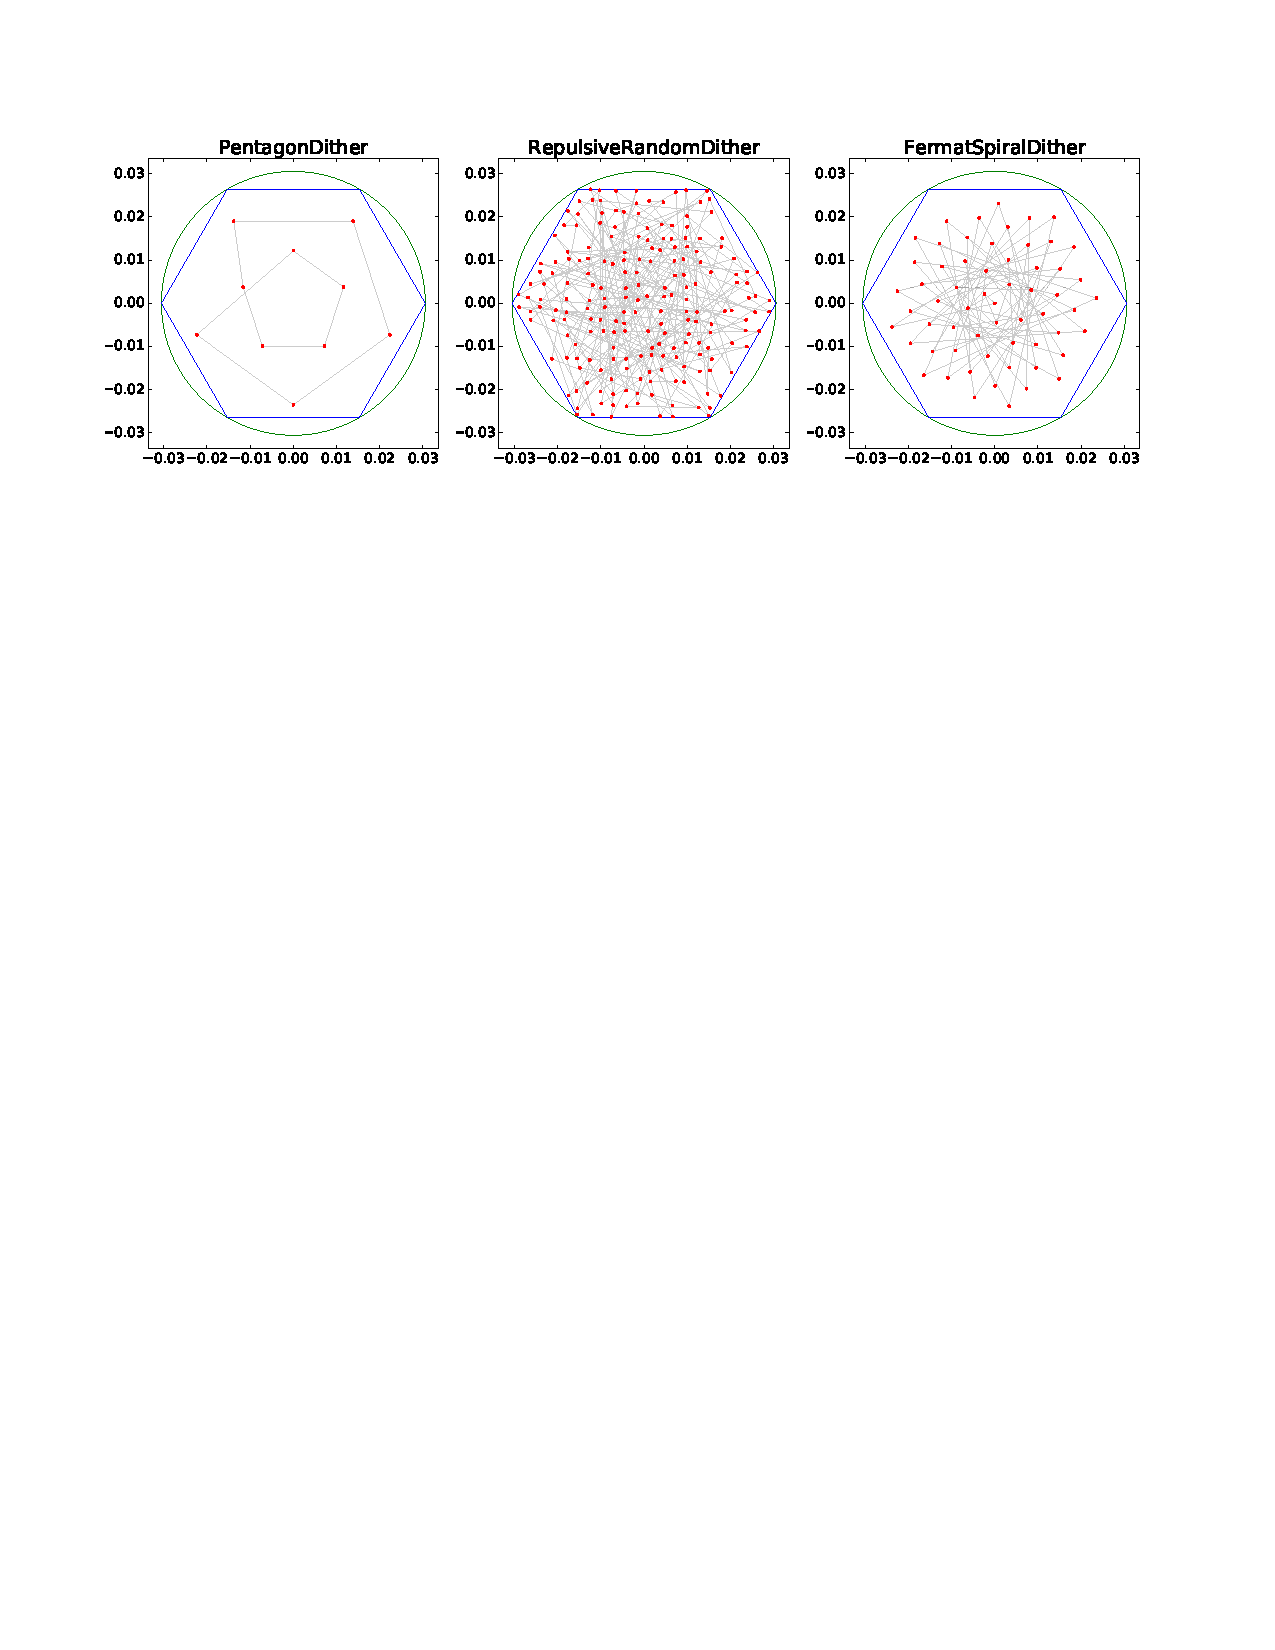
\includegraphics[width=\linewidth, trim={25 570 25 50},clip=true]{figs/awan_dithGeometries.pdf}
\caption{Dither geometries implemented for various timescales. PentagonDither is implemented only on PerSeason timescale, while the rest are implemented on FieldPerVisit, FieldPerNight, and PerNight timescales. Here the green curve is the LSST FOV of radius 0.305 radians; the blue hexagon represents the hexagonal tiling of the sky originally adopted for the undithered observations; and the red points are the dithers. The axes are in radians.}
\label{fig: dithGeometries}
\end{figure*}

Here we note that all the dithers are restricted to lie within the hexagons inscribed in the 3.5$^\circ$ LSST FOV, and that we continue with the naming scheme [Geometry]Dither[Field]Per[Timescale], where the absence of the tag `Field' implies that all fields are assigned the same dither.

% ====================================================================
% Subsection: Metrics
% ====================================================================
\subsection{Metrics}
\label{sec:\secname:metrics}
Our first metric is the \href{https://github.com/lsst/sims_maf/blob/master/python/lsst/sims/maf/metrics/simpleMetrics.py}{CoaddM5Metric}, which we use to calculate the coadded 5$\sigma$ depth resulting from various observing strategies. This allows us to compare the artifacts in the coadded depth induced by the observing strategy. Then we account for the dust extinction, using \href{https://github.com/lsst/sims_maf/blob/master/python/lsst/sims/maf/metrics/exgalM5.py}{ExGalM5Metric}, before estimating the number of galaxies in each pixel at a particular depth. For this purpose, we use a mock LSST catalog \citep{MunozEtal2015} to estimate the power law coefficients for each redshift bin, converting the depth into an estimated number of galaxies for each pixel \citep[Eq. 2]{AwanEtal2016}:
\begin{equation}
	N_{\mathrm{gal}}= 0.5\int_{-\infty}^{m_\mathrm{{max}}} {\mathrm{erfc}[a(m-5\sigma_{\mathrm{stack}})] 10^{c_1m + c_2}dm}
	\label{eq: Ngal}
\end{equation}

Here the \texttt{erfc} function accounts for incompleteness while the constants c$_1$ and c$_2$ are determined from the mock catalog. $m_{\mathrm{max}}$ specifies the magnitude cut, and we modify both $m_\mathrm{{max}}$ and c$_2$ to account for colors (assumed to be $u-g= g-r= r-i= 0.4$). This calculation is carried out using the \href{https://github.com/humnaawan/sims_maf_contrib/blob/master/mafContrib/galaxyCountsMetric_extended.py}{GalaxyCountMetric}.

We then account for the effects of photometric calibrations in our estimated number of galaxies. As discussed in \citet{AwanEtal2016}, we model the calibration uncertainties using a simple ansatz relating the systematic errors in each pixel to the seeing in that pixel (relative to the average seeing across the survey region; $\Delta s_{i}$)  and number of observations $N_{\mathrm{obs},i}$:
\begin{equation}
	\Delta_{i}= \frac{k \Delta s_{i}}{\sqrt{N_{\mathrm{obs}, i}}}
\end{equation}
where $k$ is a constant such that $\sigma_{\Delta_i}$ matches the LSST photometric calibration goal of 1$\%$  \citep{2009arXiv0912.0201L}. Since the calibration uncertainties are pixel-dependent, we use the \href{https://github.com/humnaawan/sims_maf_contrib/blob/master/mafContrib/galaxyCounts_withPixelCalibration.py}{pseudo-GalaxyCountsMetric}, which handles pixel-by-pixel calculation to modify the upper limit in the integral in \autoref{eq: Ngal} to be $m_{\mathrm{max}} + \Delta_{i}$, thereby accounting for the fluctuations in the galaxy counts due to the calibration errors. We then calculate the fluctuations in the galaxy counts in each pixel, $\delta_i= \Delta N_i/\overline{N}$.

% ====================================================================
% Subsection: Figure of Metric
% ====================================================================
\subsection{Figure of Merit}
\label{sec:\secname:FoM}
As derived and discussed in \citet{AwanEtal2016}, the spurious power from the artificial fluctuations in the galaxy counts induced by the observing strategy (OS) represents a bias in our measurement of the LSS. Hence, the uncertainty in this bias becomes the limiting factor in our ability to correct for the OS-induced structure. More quantitatively, for an optimized LSS study, the OS-induced uncertainties, \sigmaOS, must be subdominant to the statistical uncertainty \statFloor\ inherent to the measured power spectrum due to ``cosmic variance'' \citep{Dodelson}:
\begin{equation}
	\Delta C_\ell= C_{\ell,\mathrm{LSS}} \sqrt{\frac{2}{f_{\mathrm{sky}} (2\ell + 1)}}
	\label{eq: statFloor}
\end{equation}
where $f_{\rm{sky}}$ is the fraction of the sky observed, accounting for the reduction in the observed information due to incomplete sky coverage.

Since we do not include any input LSS in our pipeline, the power spectrum we measure for any given band is due to the OS-induced power, \CellOS, for that band. Modeling the overall OS-induced bias as an average across $ugri$ bands, we calculate the OS-induced uncertainties \sigmaOS\ as the standard deviation across \CellOS\ for $ugri$ bands to account for the effects of detecting the galaxy catalog through various bands. We then compare these uncertainties with the statistical floor for various redshift bins, where the statistical floor is based on the galaxy power spectra calculated using the code from \citet{Zhan2006}, which we pixelize to match the HEALPix resolution to account for the finite angular resolution of our simulations.

To quantify the effectiveness of each observing strategy in minimizing \sigmaOS, we construct a Figure of Merit (FoM) as the ratio of the ideal-case uncertainty in the measured power spectrum and the uncertainty where shot noise and OS-induced structure also play a role:
\begin{equation}
	\mathrm{FoM} = \sqrt{\frac{\sum\limits_\ell{\left({\sqrt{\frac{2}{f_{\mathrm{sky, max}} (2\ell + 1)}}C_{\ell, \mathrm{LSS}}} \right)}^2}{\sum\limits_\ell \left[{ \left( { \sqrt{\frac{2}{f_{\mathrm{sky}} (2\ell + 1)}}\left\{{C_{\ell, \mathrm{LSS}} + \frac{1}{\bar{\eta}}} \right\}  } \right ) ^2 + \sigma_{C_{\ell,\mathrm{OS}}}^2  }\right]}}
\label{eq: FoM}
\end{equation}
Here, $\bar{\eta}$ is the surface number density in steradians$^{-1}$, and the term containing it accounts for the contribution from the shot noise to the measured signal \citep{HutererEtal2001,Jing2005}. This FoM measures the percentage of ideal-case information that can be measured in the presence of systematics. We note that the shot noise is negligible even for the shallowest (10-year) surveys we consider.

We define the ideal-case as being based on the largest coverage of the sky with LSST, i.e., $f_{\rm{sky, max}}$ is the largest WFD coverage with the baseline cadence. For \opsimdbref{db:baseCadence}, the observing strategy with RepulsiveRandomDitherFieldPerVisit dithers leads to the largest $f_{\rm{sky}}$ ($\sim 39.5\%$). Note that this fraction is calculated after masking the shallow borders of the main survey; for details, see \citet{AwanEtal2016}. %Therefore, we fix the $f_{\rm{sky, best}}$ to be $39.5\%$ and compare the the different observing strategies and cadences relative to it. 

% ====================================================================
% Subsection: A Comment on Terminology
% ====================================================================
\subsection{A Comment on Terminology}
For clarity, we make a note on the terminology we have introduced. Strictly speaking, the bias caused by the observing strategy is a window function bias, as the survey window function ($W_i$) accounts for the effective survey geometry which scales the fluctuations in the galaxy counts in each pixel: $1+\delobs= W_i(1+\dellss)$. Comparing this with Equation 4 in \citet{AwanEtal2016}, $1+\delobs= (1+\delos)(1+\dellss)$, we see that the OS-induced bias is directly related to the window function: $1 + \delos= W_i$

Then, for the total power, we have
\begin{equation}
\ev{\delobs^2}=\ev{\dellss^2}\ev{(1 + \delos)^2}+ \ev{\delos^2}=\ev{\dellss^2}\ev{W_i^2}+ \ev{(W_i-1)^2}
\end{equation}
where the first equality is based on Equation 6 in \citet{AwanEtal2016} and the second one holds given the relation between $\delos$ and $W_i$. Since the OS-induced bias $\delos^2=  (W_i-1)^2$, the uncertainties in the OS-induced bias are the window function uncertainties.

Generally the window function is assumed to be known perfectly and its uncertainties are not explicitly identified as such. To avoid confusion and focus on the window function uncertainties arising from the observing strategy, we continue using the term OS-induced bias and its uncertainties in favor of window function and its uncertainties.

% ====================================================================
% Subsection: OpSim Analysis and Results
% ====================================================================
\subsection{OpSim Analysis and Results}
\label{sec:\secname: analysis}
For the purposes of our analysis, we use HEALPix resolution of $N_\mathrm{_{side}}= 256$, effectively tiling each $3.5^\circ$ FOV with about 190 HEALPix pixels. Using the metrics discussed in \autoref{sec:\secname:metrics}, we analyze \sigmaOS\ from various observing strategies. First we present the results for the baseline cadence, \opsimdbref{db:baseCadence}.

\begin{figure*}[!htb]
      \centering\hspace*{-3em}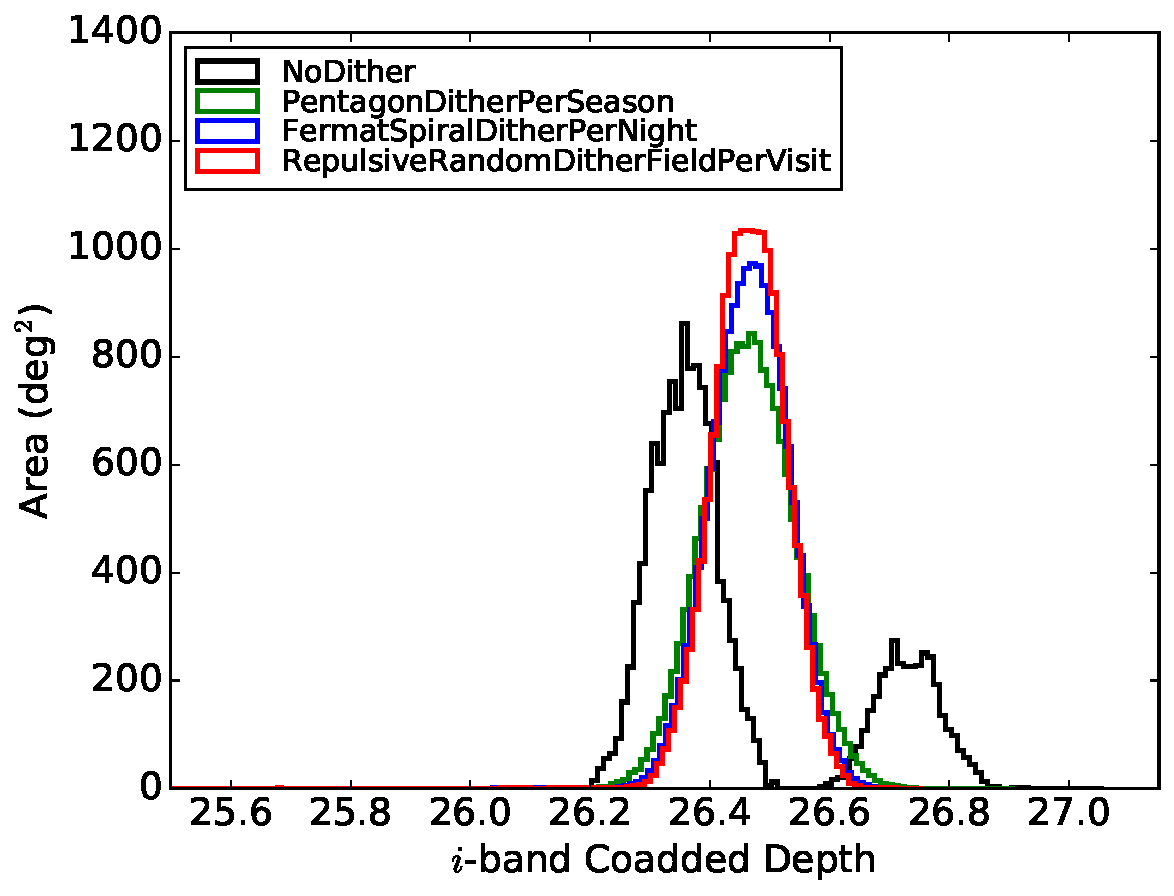
\includegraphics[width=0.6\linewidth]{figs/awan_coaddHistogram.pdf}
      \vspace*{-1em}
\caption{Histogram for the $i$-band coadded 5$\sigma$ depth after the full, 10-year survey.}
\label{fig: coaddHistogram}
\end{figure*}

\autoref{fig: coaddHistogram} shows the histogram for the $i$-band coadded 5$\sigma$ depth from \opsimdbref{db:baseCadence} for the four observing strategies. We observe a bimodal distribution for the undithered survey -- the deeper depth mode corresponds to the overlapping regions between the hexagons, while the rest of the survey contributes to the shallower mode. In contrast, all dithered surveys lead to unimodal distributions as the overlapping regions between the fields change frequently, leading to more uniformity. We also note that frequent dithering leads to deeper regions as we observe more peaked histograms for FieldPerVisit and PerNight strategies.

\autoref{fig: coaddSkymaps} shows the plots for the $i$-band coadded 5$\sigma$ depth for the observing strategies. As in \citet{AwanEtal2016}, we find that the undithered survey leads to a strong honeycomb pattern which is much weaker in all of the dithered surveys. We again observe that the dithered surveys are deeper than the undithered survey in terms of the median depth across the survey region.

\begin{figure*}[!htb]
      \centering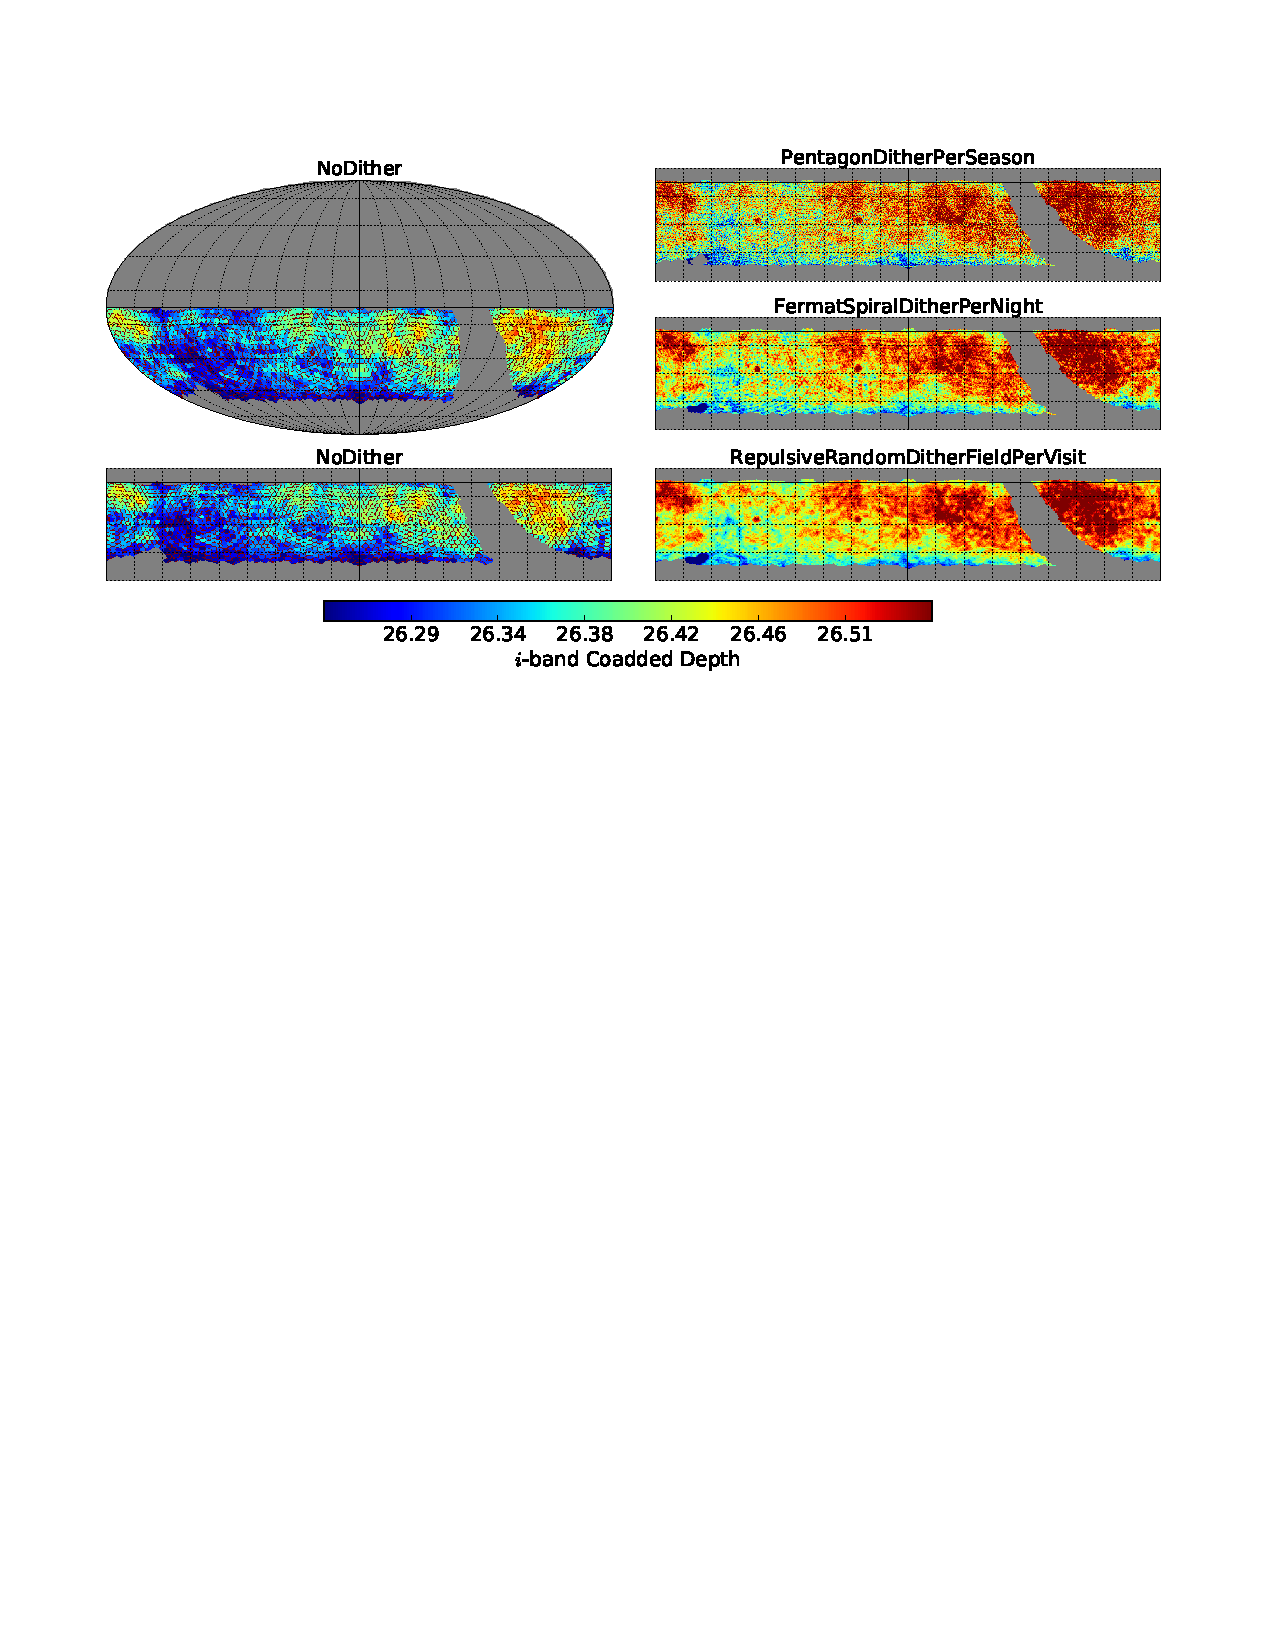
\includegraphics[width=\linewidth, trim={50 470 55 70},clip=true]{figs/awan_minion1016_coaddSkymaps.pdf}
\caption{Plots for the $i$-band coadded 5$\sigma$ depth based on \opsimdbref{db:baseCadence} for various observing strategies. The top left plot shows the Mollweide projection for NoDither while the bottom left shows the corresponding Cartesian projection, restricted to $180^\circ>$RA$>-180^\circ$ (left-right), $-70^\circ<$Dec$<10^\circ$ (bottom-top). Only the latter is shown for the rest of the strategies. }
\label{fig: coaddSkymaps}
\end{figure*}

In order to quantify the angular characteristics observed in the skymaps, we calculate the angular power spectra corresponding to the skymaps for the $i$-band coadded 5$\sigma$ depth. \autoref{fig: coaddPowerSpectrum} shows these spectra for the four observing strategies. We observe a sharp reduction in the artificial power in the dithered surveys when compared to the undithered one: the strong honeycomb pattern in the undithered survey leads to a large peak around $\ell\sim150$, while the peak is about 10 times weaker in the dithered surveys. We do, however, observe variations amongst the various dither strategies: while RepulsiveRandom dithers lead to small power for all timescales, PerSeason dithers lead to large power on larger angular scales, and both PerSeason and FermatSpiral lead to large power around $\ell\sim150$ (which still is $<10\times$ the corresponding peak from the undithered survey).

\begin{figure*}[!htb]
      \centering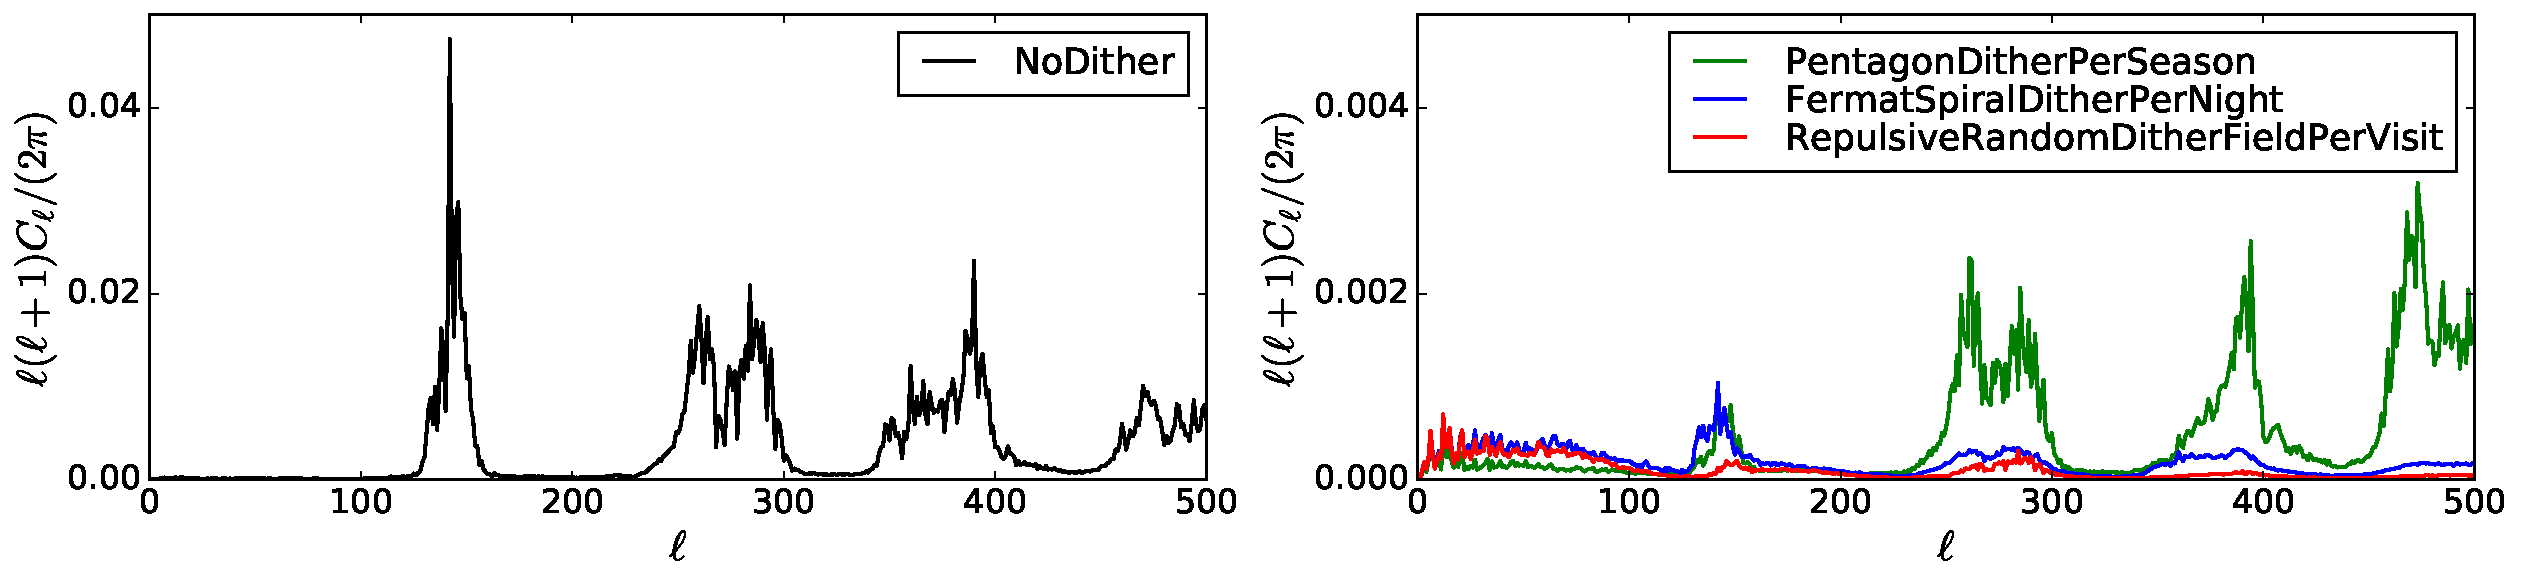
\includegraphics[width=\linewidth]{figs/awan_coaddpowerspectrum.pdf}
      \vspace*{-2em}
\caption{Angular power spectra for the  $i$-band coadded 5$\sigma$ depth from \opsimdbref{db:baseCadence} for various observing strategies. We note that dithering reduces the spurious power by over 10$\times$.}
\label{fig: coaddPowerSpectrum}
\end{figure*}

We then proceed to calculate the OS-induced bias and its uncertainty from the different observing strategies. First, we examine simulated results after only one year of survey. \autoref{fig: minion1016: 1yr} shows the comparison between \sigmaOS\ and \statFloor\ for $0.66<z<1.0$ after the 1-year survey for two magnitude cuts: $i<24.0$ and $i<25.3$. We observe that the undithered survey leads to \sigmaOS\ 1-5$\times$ the statistical floor around $\ell\sim150$; PerSeason timescale does only slightly better. However, we see an improvement with frequent dithers: both FieldPerVisit and PerNight implementations lead to uncertainties 0.5-1$\times$ the statistical floor, although FermatSpiral dithers on PerNight timescale lead to a peak around $\ell\sim150$ more pronounced than the one from RepulsiveRandom dithers on FieldPerVisit timescale.

\begin{figure*}[!htb]
      \centering\hspace*{1em}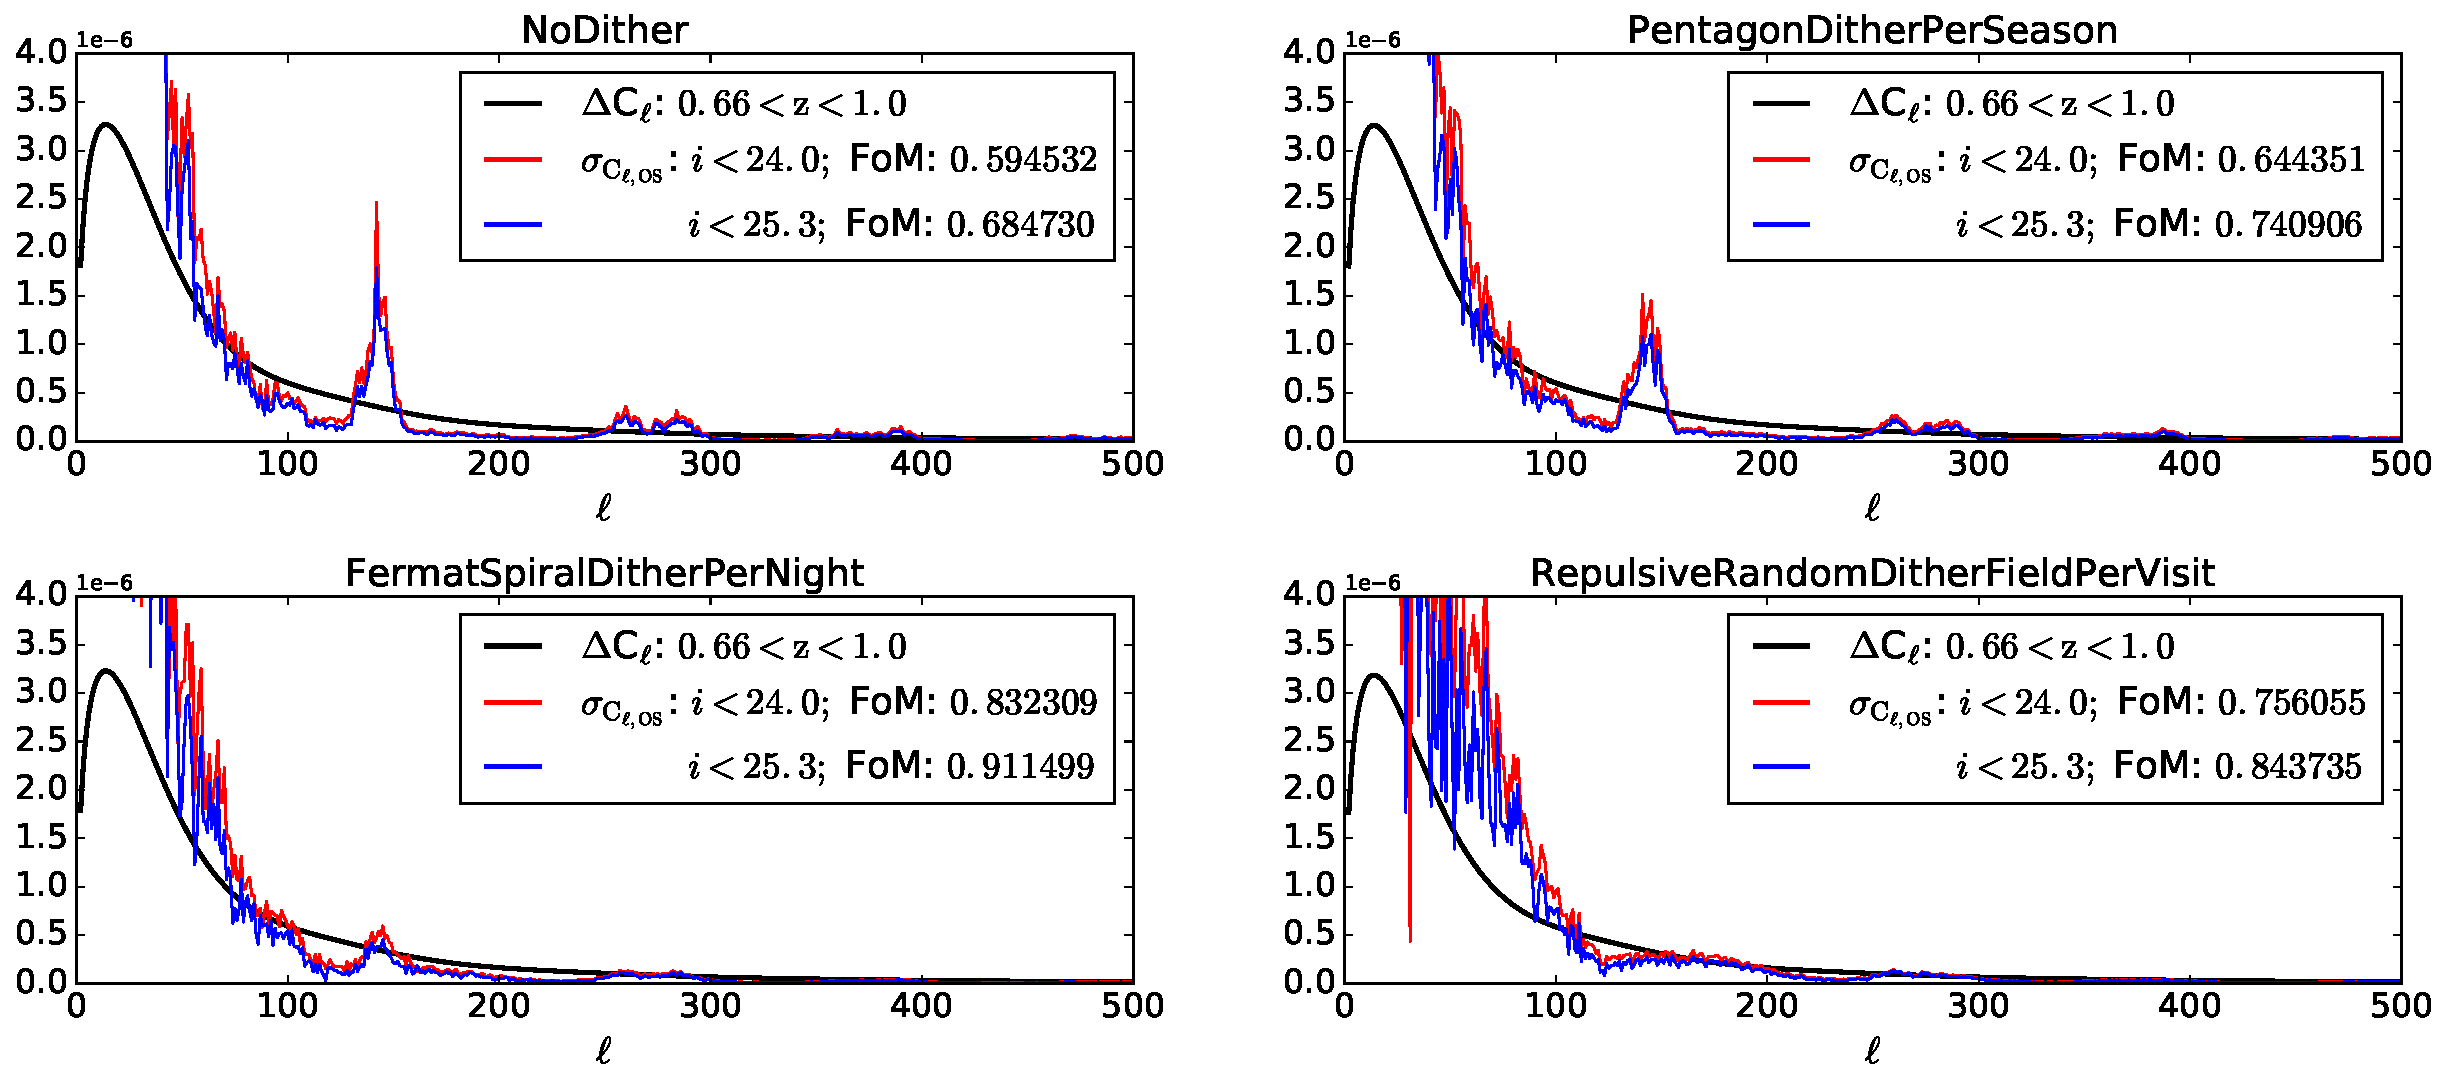
\includegraphics[width=\linewidth]{figs/awan_1yr_minion1016_2magCuts.pdf}
       \vspace*{-2em}
\caption{\sigmaOS\ comparison with the minimum statistical uncertainty \statFloor\ for $0.66<z<1.0$ for different magnitude cuts after only one year of survey based on \opsimdbref{db:baseCadence}.}
\label{fig: minion1016: 1yr}
\end{figure*}

The trends are captured in the Figure of Merit, which we calculate using \autoref{eq: FoM} over the range $100<\ell<300$. We observe a smaller FoM for the shallower survey -- realistic given that although there is less structure and therefore weaker OS-induced artifacts, the shot noise becomes significant and makes the FoM smaller. For the deeper survey, we find that FermatSpiralDitherPerNight outperforms all others with the highest FoM, while RepulsiveRandomDitherFieldPerVisit is more effective than PerSeason dithers. The undithered survey, as expected, performs the worst.

In \autoref{fig: minion1016: 10yr}, we show simulated results after the full, 10-year survey for $0.66<z<1.0$ for three different magnitude cuts: $i<24.0$, $i<25.3$ and $i<27.5$. We observe stark differences between the undithered and dithered surveys: the former leads to large uncertainties in the OS-induced bias while the latter is effective in bringing \sigmaOS\ well below the statistical floor. The effectiveness of all three dithered surveys in minimizing the uncertainties implies more flexibility in choosing the dither strategy for years 2-10.

%For 10yr, 3 magnitude cuts with minion1016, NoDither was always bad but PerSeason dithers were giving us comparable FoM to PerNight and FieldPerVisit dithers. That is not the case anymore; PerSeason dithers are now doing slightly better than before though still not as good as PerNight and FieldPerVisit dithers.

Analyzing the FoM more closely, we observe that the gold sample leads to smaller FoM than both the shallower and deeper catalogs. The larger FoM for shallower catalog is realistic, given less structure with shallow depth leads to weaker artifacts and the shot noise is negligible over the full ten-year survey, but the out-of-trend behavior of gold sample hints at a peculiarity of the variance across the $ugri$ bands at that depth for the baseline cadence. We investigate this behavior briefly and find that the $u$-band-induced artifacts add the most to the uncertainties in the bias induced by the observing strategy, as the gold sample $u$-band cadence in the \opsimdbref{db:baseCadence} is different from $gri$ cadences. This issue still needs to be further investigated, with potentially incorporating the importance of each band to calculate an overall OS-induced bias. We note, however, that this peculiarity is particularly enhanced for the undithered survey.

\begin{figure*}[!htb]
      \centering\hspace*{1em}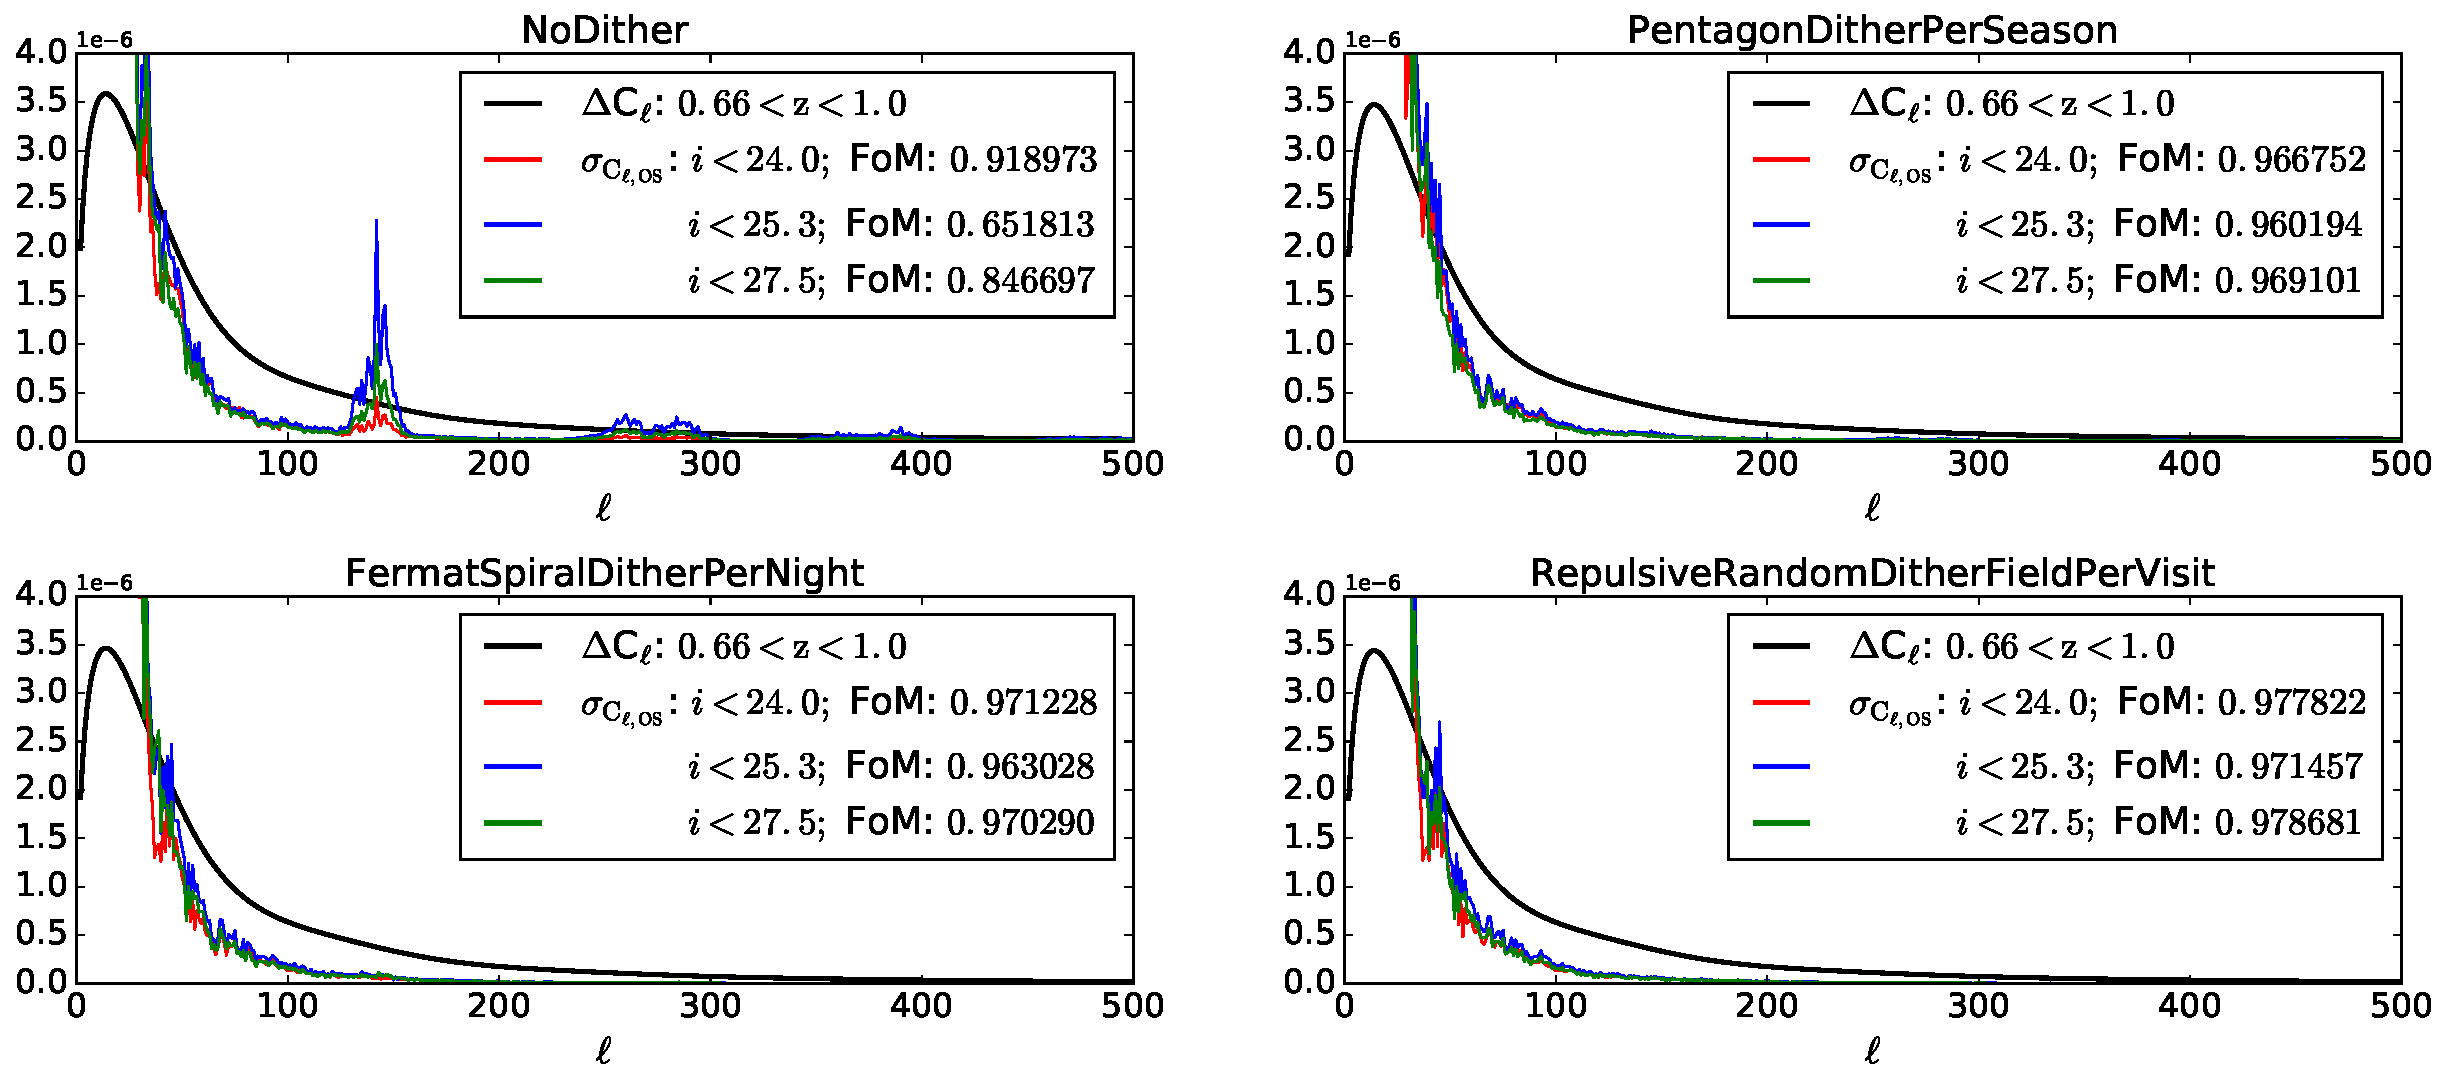
\includegraphics[width=\linewidth]{figs/awan_10yr_minion1016_3magCuts.pdf}
       \vspace*{-2em}
\caption{\sigmaOS\ comparison with the minimum statistical uncertainty \statFloor\ for $0.66<z<1.0$ for different magnitude cuts after the full, 10-year survey based on \opsimdbref{db:baseCadence}.}
\label{fig: minion1016: 10yr}
\end{figure*}

The trends observed here remain consistent for all five redshift bins. We note that our choice of dithers is particularly important for the one-year survey as only one of the three dither strategies leads to a large FoM. Therefore, in the absence of effective dithers, systematics correction methods will become necessary after the one-year survey. However, these methods may not lead to significant improvements for a dithered 10-year survey as dithers of most kinds are effective in reducing the uncertainties well below the minimum statistical limit.

To further probe the effects of dithers, we run the 1-year and 10-year analyses for two cadences besides the baseline cadence: \opsimdbref{db:NoVisitPairs} which does not require visit pairs, and \opsimdbref{db:opstwoPS} which implements a Pan-STARRS-like observing strategy offering a larger area coverage. In \autoref{fig: cadences: 1yr}, we compare the results from these two cadences with those from \opsimdbref{db:baseCadence} for $0.66<z<1.0$ for the  $i<25.3$ galaxy sample after only one year of survey. We see that the undithered survey leads to large uncertainties in the OS-induced bias with all three cadences, with the peak uncertainty 5-15$\times$ the statistical floor. As expected, the undithered survey with the wider coverage \opsimdbref{db:opstwoPS} cadence leads to stronger artifacts and a much smaller FoM (by $\sim33\%$ in comparison with \opsimdbref{db:baseCadence}), while not requiring visit-pairs is slightly more effective than the baseline (FoM increases by about 6$\%$). We see very similar trends for the three cadences for PerSeason dithers although the peak \sigmaOS\ ranges between 3-9$\times$ the statistical floor; FoM based on \opsimdbref{db:opstwoPS} is worse than that from \opsimdbref{db:baseCadence} by about 25$\%$ and  \opsimdbref{db:NoVisitPairs} improves on the baseline FoM by $\sim5\%$.

% For different cadences, 1yr results, we now have FoM really high for the wider minion1020 for both PerNight and FieldPerVisit dithers while NoDither and PerSeason dithers are still performing poorly. RepRandom dithers with the wider survey gets us F0M=0.99 while FermatSpiral dithers perform better than RepRandom for the other two cadences.

As before, \sigmaOS\ improves with more frequent dithering. It is only about 1-3$\times$ the statistical floor for FermatSpiral dithers on PerNight timescale. In contrast to NoDither and PerSeason dithers, both \opsimdbref{db:opstwoPS} and \opsimdbref{db:NoVisitPairs} perform better than baseline\opsimdbref{db:baseCadence} with PerNight dithers: FoM from the wider coverage cadence is about $4.5\%$ better than for the baseline cadence, while we see a $4\%$ better FoM with \opsimdbref{db:NoVisitPairs}. 

For RepulsiveRandom dithers on FieldPerVisit timescale, we find that the uncertainties in the OS-induced bias are on the same scale as the statistical floor. The wider coverage cadence outperforms the baseline cadence significantly as  the wider survey FoM is about $18\%$ better than the baseline FoM while the improvement is about 3$\%$ when not requiring visit-pairs. We emphasize that the differences between results with different cadences is highly dependent on the observing strategy: the wider coverage with no or infrequent dithers performs quite poorly while it significantly improves the FoM when large, frequent dithers are implemented. On the other hand, not requiring visit-pairs leads to comparatively larger improvement for infrequent dithers than frequent ones (compared to the baseline).

\begin{figure*}[!htb]
      \centering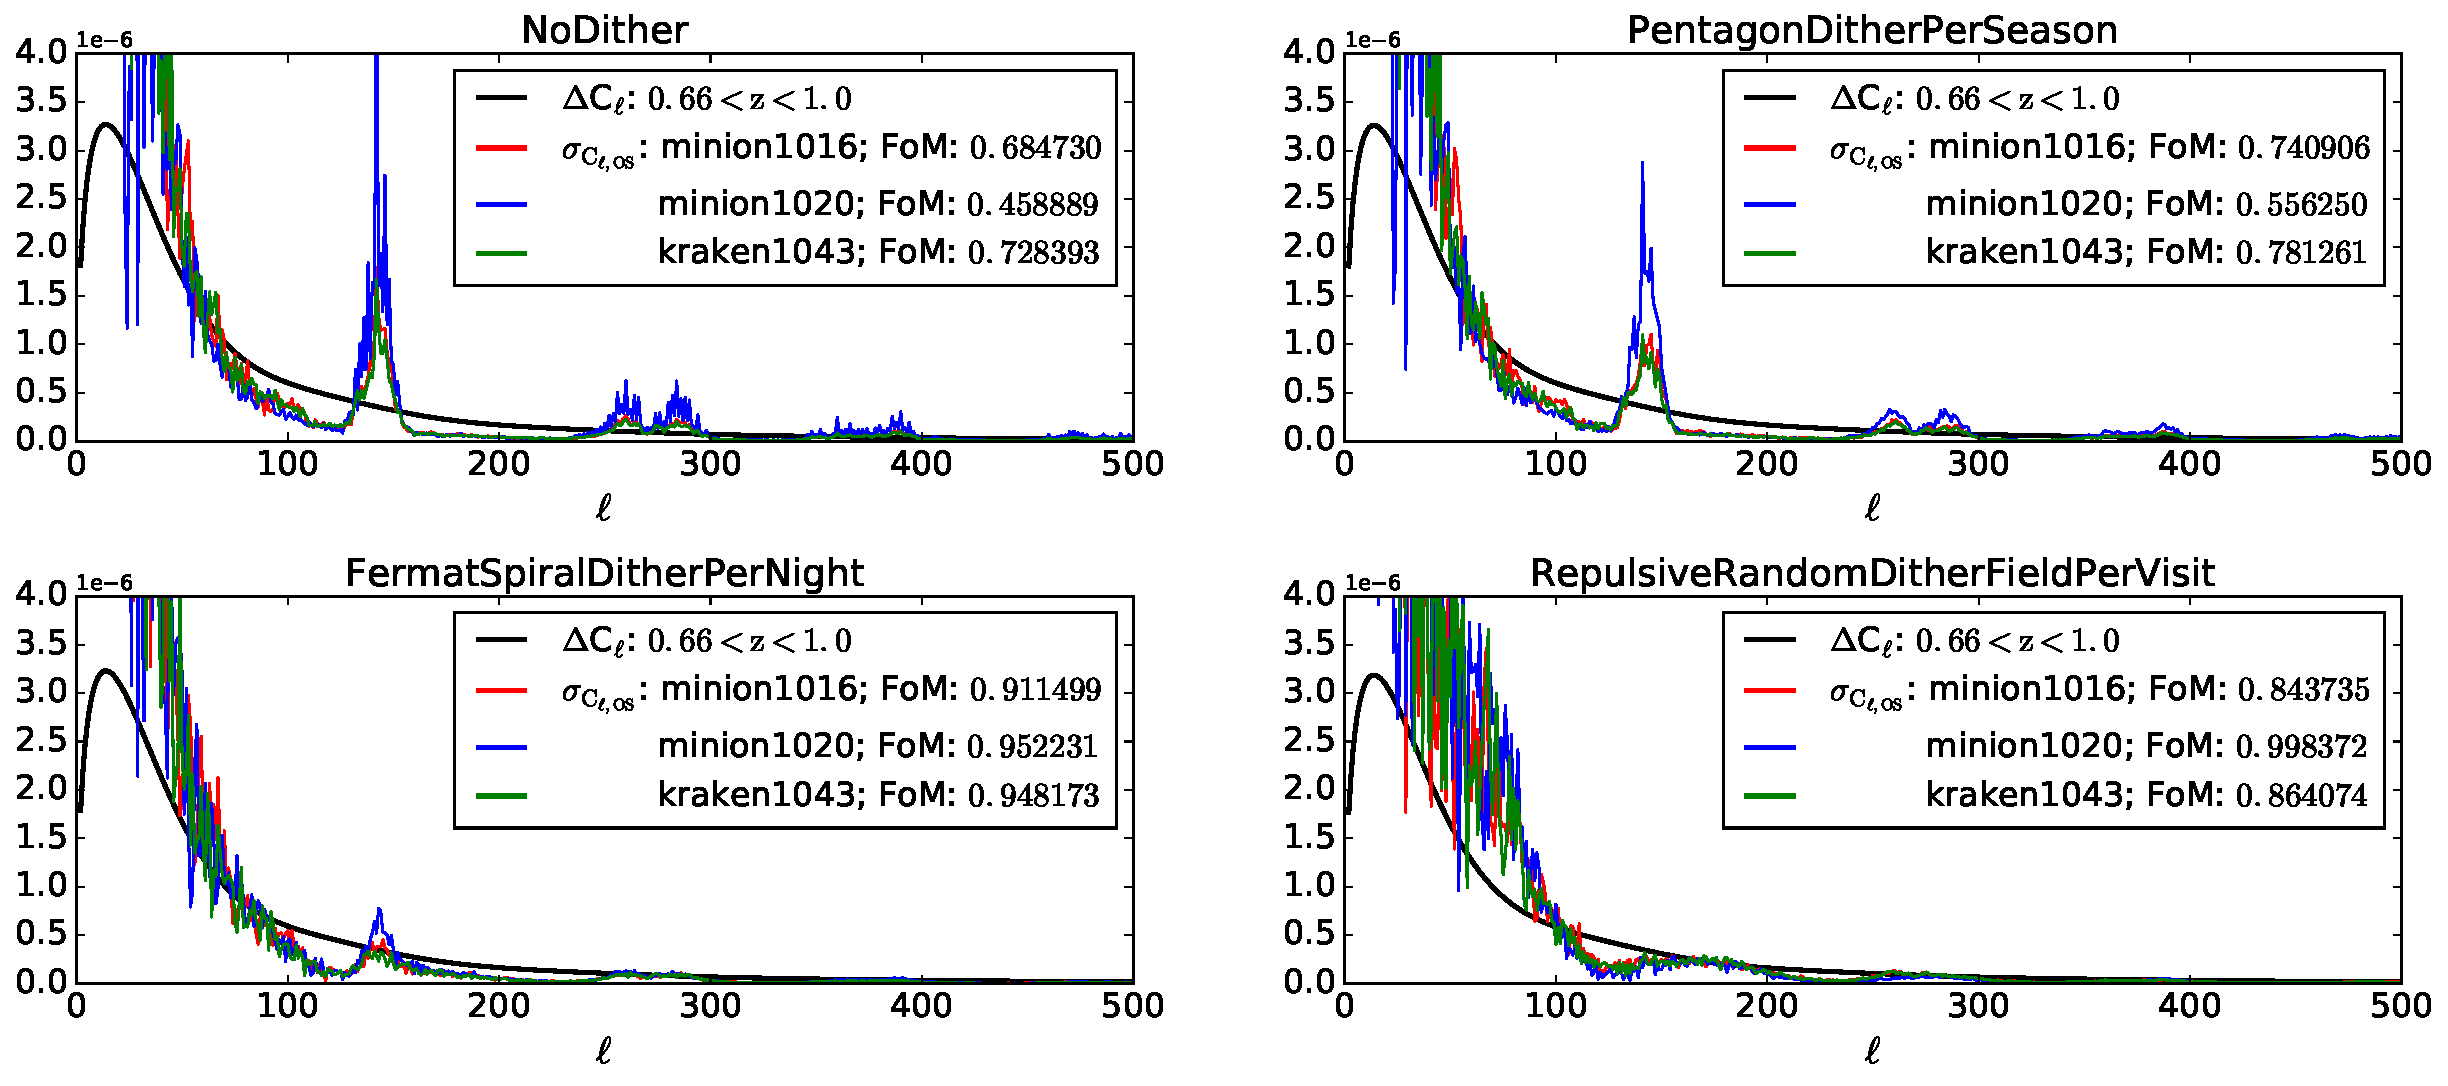
\includegraphics[width=\linewidth]{figs/awan_1yr_goldSample_3cadences.pdf}
       \vspace*{-2em}
\caption{\sigmaOS\ comparison with the minimum statistical uncertainty \statFloor\ for $0.66<z<1.0$ for three different cadences for $i<25.3$ after only one year of survey.}
\label{fig: cadences: 1yr}
\end{figure*}

Finally, we show the simulated results for different cadences after the 10-year survey in \autoref{fig: cadences: 10yr}. As in \autoref{fig: minion1016: 10yr}, we see that all the dithered surveys effectively minimize the uncertainties, regardless of the cadence. We do observe, however, that the wider coverage \opsimdbref{db:opstwoPS} still underperforms significantly for the undithered survey (FoM about 30$\%$ less than baseline FoM)  while all the dithered surveys see a stark improvement (FoM $>$ 1 for all; $\sim 20\%$ improvement on the baseline FoM). The improvement from \opsimdbref{db:NoVisitPairs} is comparable among the four observing strategies. Based on these results, we note than wider coverage offers significant improvements with large dithers on any implementation timescale.

\begin{figure*}[!htb]
      \centering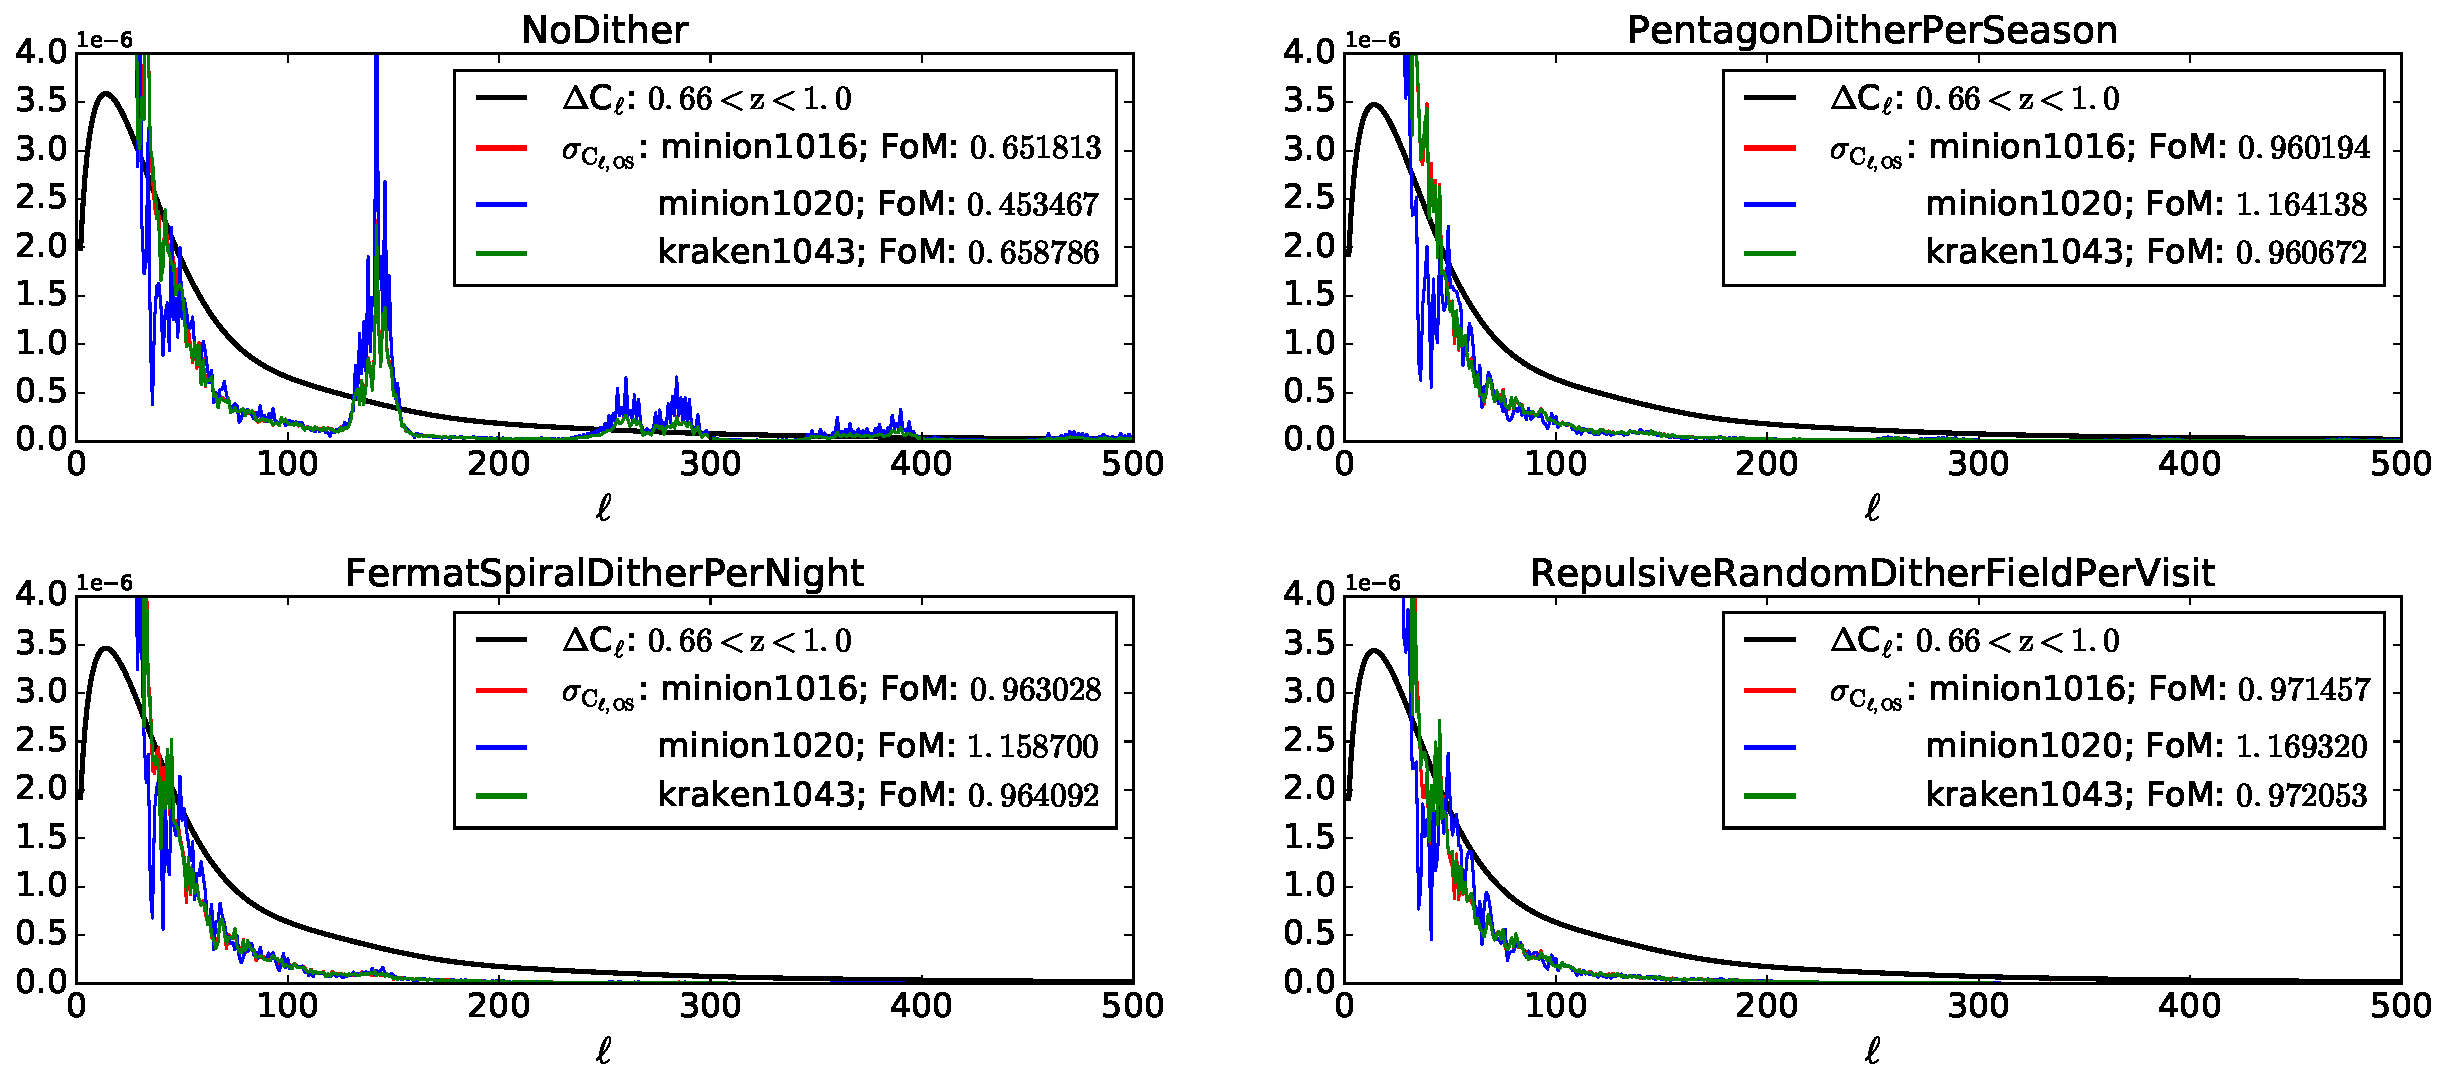
\includegraphics[width=\linewidth]{figs/awan_10yr_goldSample_3cadences.pdf}
       \vspace*{-2em}
\caption{\sigmaOS\ comparison with the minimum statistical uncertainty \statFloor\ for $0.66<z<1.0$ for three different cadences for $i<25.3$ after the full, 10-year survey.}
\label{fig: cadences: 10yr}
\end{figure*}

% ====================================================================
% Science Case Conclusions
% ====================================================================
\subsection{Conclusions}

Here we answer the ten questions posed in
\autoref{sec:intro:evaluation:caseConclusions}:

\begin{description}

\item[Q1:] {\it Does the science case place any constraints on the
tradeoff between the sky coverage and coadded depth? For example, should
the sky coverage be maximized (to $\sim$30,000 deg$^2$, as e.g., in
Pan-STARRS) or the number of detected galaxies (the current baseline but
with 18,000 deg$^2$)?}

\item[A1:] As we see in \autoref{sec:\secname: analysis}, a deeper
catalog is more effective, though it makes the choice of the dither
strategy more important, especially in the first year of survey. We also see 
that the wider-coverage cadence \opsimdbref{db:opstwoPS} performs 
significantly better for LSS systematics with large, frequent dithers  
while it performs much poorly with no or infrequent dithers; this
trend is consistent for both one-year and the full, ten-year surveys. We
note here that one year of the wider coverage (for gold sample) with frequent large
dithers leads to better systematics (as quantized here) than ten years of 
the standard WFD  footprint, strongly supporting the effectiveness of wider area
coverage in the first year of survey for LSS systematics. We are definitely area-
limited more than depth-limited for LSS studies.

\item[Q2:] {\it Does the science case place any constraints on the
tradeoff between uniformity of sampling and frequency of  sampling? For
example, a rolling cadence can provide enhanced sample rates over a part
of the survey or the entire survey for a designated time at the cost of
reduced sample rate the rest of the time (while maintaining the nominal
total visit counts).}

\item[A2:] Depth uniformity is critical for LSS systematics. As we
demonstrated in \autoref{sec:\secname: analysis}, LSS studies will benefit
strongly from large dithers and wide area coverage. We do not have constraints
on the cadence.

\item[Q3:] {\it Does the science case place any constraints on the
tradeoff between the single-visit depth and the number of visits
(especially in the $u$-band where longer exposures would minimize the
impact of the readout noise)?}

\item[A3:] From our investigation into the large uncertainties in the
OS-induced bias observed in the gold sample in the baseline cadence, in
comparison with the shallower and deeper catalogs, we find that
$u$-band-induced artifacts add the most to the uncertainties in the
bias. Hence there could be a significant penalty from reducing the
number of $u$-band visit. At minimum, doing so would make the choice of
dither pattern more important. This issue still needs to be further
investigated.

\item[Q4:] {\it Does the science case place any constraints on the
Galactic plane coverage (spatial coverage, temporal sampling, visits per
band)?}

\item[A4:] LSS systematics do not place any constraints on the Galactic
plane coverage.

\item[Q5:] {\it Does the science case place any constraints on the
fraction of observing time allocated to each band?}

\item[A5:] Increasing the number of visits leads to greater survey
uniformity. At present, this is worst (among $ugri$) in the $u$-band, so
increasing the fraction of $u$-band observing time would likely help.

\item[Q6:] {\it Does the science case place any constraints on the
cadence for deep drilling fields?}

\item[A6:] LSS systematics do not constrain the cadence for deep
drilling fields as long as the main survey dithers are not affected.

\item[Q7:] {\it Assuming two visits per night, would the science case
benefit if they are obtained in the same band or not?}

\item[A7:] We do not see significant difference between obtaining two
visits per night in the same band or not, although we do see a mild
benefit in not obtaining the visits in the same band as it allows
greater variation in atmospheric conditions in each band.

\item[Q8:] {\it Will the case science benefit from a special cadence
prescription during commissioning or early in the survey, such as:
acquiring a full 10-year count of visits for a small area (either in all
the bands or in a  selected set); a greatly enhanced cadence for a small
area?}

\item[A8:] We will request full, 10-year depth during commissioning to
validate our choice of dither pattern.

\item[Q9:] {\it Does the science case place any constraints on the
sampling of observing conditions (e.g., seeing, dark sky, airmass),
possibly as a function of band, etc.?}

\item[A9:] Seeing will play a role in the photometric calibration
errors. However, these errors appear to be subdominant to the artifacts
induced by the observing strategy.

\item[Q10:] {\it Does the case have science drivers that would require
real-time exposure time optimization to obtain nearly constant
single-visit limiting depth?}

\item[A10:] We do not require any real-time exposure time optimization.

\end{description}

% ====================================================================
% Discussion
% ====================================================================
\subsection{Discussion}
\label{sec:\secname:discussion}

In this section, we presented results for the impacts of LSST observing
strategy on LSS studies. Using the OpSim cadence baseline
\opsimdbref{db:baseCadence}, we demonstrate that dithers are necessary
for both 1-year and 10-year surveys. We find that of the three dither strategies
discussed here, FermatSpiral dithers on PerNight  timescale are the most
effective for the gold sample after one-year of survey while  dithers of all kinds
are effective after the ten-year survey. These results imply the need for a very careful
choice of the observing strategy in the first year while there is quite a range of choice 
for years 2-10.

We also analyze two other cadences and find  that frequent dithering with
maximum  sky coverage could allow a significant  fraction LSST-enabled LSS
science after  one-year. Assuming that the quality of photometric redshifts is
fixed (when it actually improves with depth) and that our ansatz for window
function uncertainties is representative,  our results can go as far as implying
that the wider coverage for a few years is far more important than more years of the
baseline  WFD coverage.

Future work will entail improving our analysis to better constrain the
artifacts induced by the observing strategy by, e.g., including
uncertainties in the dust extinction, using improved models for the
photometric calibration uncertainties, more realistic galaxy colors,
incorporating improved mock catalogs to better estimate the galaxy
counts as well as its uncertainties, and a better estimate of the
uncertainties in the OS-induced by a more thorough accounting of the
effects of each band. Also, the development and the analysis of the
effectiveness of various systematics correction methods needs to be
carried out, especially for the 1-year survey, as only a few observing 
strategies reduce the artifacts. Finally, the effectiveness
of various dithers still needs to be assessed for other science probes.


\navigationbar


% --------------------------------------------------------------------

% ====================================================================
%+
% SECTION NAME:
%    wl.tex
%
% CHAPTER:
%    cosmology.tex
%
% ELEVATOR PITCH:
%-
% ====================================================================

\newcommand{\red}[1]{\textcolor{red}{#1}}

\clearpage
\section{Weak Lensing}
\def\secname{wl}\label{sec:\secname}

\credit{jmeyers314},
\credit{tonytyson}.

Much of LSST cosmology may be limited by systematic rather than statistical
errors.  This is especially true of weak gravitational lensing, which relies on
very accurate (\ie low bias), estimates of the shear of large ensembles of
galaxies. Measurements of the noisy shapes of many galaxies, and high
signal-to-noise measurements of PSF calibration stars are made.   Even though
the shot noise of the shape of an individual galaxy is very large, any small
shear bias could accumulate over many such galaxies.  As outlined in the SRD,
uniformity of seeing in the bands used for weak lensing and special observing
strategies are required in order to reduce additive and multiplicative shear
systematics.

Achieving the ultimate sensitivity of the LSST to weak lensing science places
stringent requirements on our ability to accurately estimate galaxy shapes and
redshifts, which in turn demands precise and accurate knowledge of the point
spread function, astrometry, and photometry.  These measurements are influenced
by the interaction of light with the Earth's atmosphere, the telescope optics,
and the CCD sensors.  Systematics in the shear are introduced in each case.
Observing strategies have been developed for suppressing these systematics in
current lensing surveys, such as the Deep Lens
Survey\footnote{\url{dls.physics.ucdavis.edu}}.  These and new methods will be
applied to the LSST survey.

To leading order, we can express the effect of shear systematics in the observed
shear $\gamma^\mathrm{obs}_i$ as a small linear perturbation of the true shear
$\gamma_i$,

$$ \gamma_i^\mathrm{obs} = (1+m_i) \gamma_i + c_i, $$

where $m_i$ is the multiplicative and $c_i$ is the additive systematic in the
ith shear component.  These systematics have contributions from the atmosphere
and the detector+optics.  Systematic errors in the PSF of the relatively
brighter calibration stars in the field are propagated to errors in the galaxy
shear, depending on the relative half-light sizes of the  galaxy and star.  To
leading order, the PSF contributions to the additive systematic are a linear
function of the PSF ellipticity.  The best observing strategies cause the
average PSF ellipticity at a given point (over all exposures) to average towards
zero.

From the LSST SRD requirements on residual systematics in the galaxy shear-shear
correlation function one can specify the level of residual shear systematics at
which statistical uncertainties become subdominant.  Over the sample of 3-4
billion galaxies, the shear systematics must be below 3 parts in 10,000 for
additive shear $|c|$, and 3 parts in 1000 for multiplicative shear $|m|$.  Each
visit to a sky patch encounters these systematics.  In particular, each re-visit
to a given field generates the same CCD-based additive shear systematic.  Some
observing strategies can effectively randomize these over all visits to a field.
It is important to note that the full survey shear-shear correlation error due
to these systematics is expected to be no better than the corresponding
systematic in any given field after all re-visits to that field. This is because
the useful angular scales in cosmic shear are less than a field radius of
several degrees, and the systematics floor in shear-shear correlation is set
therefore by the floor in any one typical field.  Below we discuss the observing
strategies for suppressing shear systematics and metrics for their success.


\subsection{Target Selection}

Image quality must be uniformly good in the bands used for weak lensing shear.
These will be mainly the $r$ and $i$ bands, though it is possible that the $z$
band will also be used for shear measurement.  The decision on which field to
observe next must be based mainly on its weak lensing priority \citep[Sec 3.1
and Figure 14.4]{2009arXiv0912.0201L}.  Depending on the current weather and
seeing, the scheduler will have a list of priorities for next-field, based on
prior history of coverage.  The relevant parameters are seeing, depth, and
camera rotation angle with respect to North and to zenith. Nearby fields in need
of coverage in these bands should be given high priority if the seeing is better
than some specified value, likely 0.7 arcsec FWHM \citep[Sec
14.5.2]{2009arXiv0912.0201L}.

\subsection{Target Measurements}

It is expected that even after optimization of camera optics and electronics,
systematic image shape errors will be associated with the orientation of the
camera focal plane.  Using data from vendor CCDs, simulations of LSST observing
have shown that a combination of x-y dithering on the sky and pipeline
processing with pixel re-map (to cancel much of the CCD frame fixed distortions)
can get well within a factor of ten of the goal for shear systematics residuals.
Simulations which add camera angle dithering show that the residual shear
systematics goal can be achieved in fields with relatively uniform seeing
history \citep{Jee&Tyson2011}.  To average down the PSF systematics over many
re-visits we benefit from uniformly distributed image quality over the ensemble.
A non-uniform history in some field can be addressed by the scheduler taking
that into account for the offending rotation angle(s) in the history of prior
visits.

Thus shear systematics will be reduced by randomization of the orientation of
the camera with respect to the sky.  This is represented by the parameter
RotSkyPos, defined as the angle between the $+y$ camera direction and North.  We
can construct diagnostic metrics that quantify the uniformity of its
distribution at each sky position.  Given the spin 2 symmetry of shear, the
optimal strategy for shear systematics will be to aim for uniformity of
RotSkyPos mod $\pi$, since angles separated by $\pi$ radians are degenerate.

Similarly, the telescope optics may harbor systematic aberrations, and these
also could be mitigated by recording images with a uniform distribution of
parallactic angle, which is the angle between North and zenith for a given field
observation.  Differential chromatic refraction (DCR) effects will also be
mitigated by varying the parallactic angle, though the exact relationship is
complex since the parallactic angle sets both the DCR magnitude and direction
for a given observation.  Re-visits to a given field should be distributed over
parallactic angles (or equivalently, hour angles), consistent with airmass and
seeing limits.  Note that wide hour angle coverage for a given field will also
be helpful in order to efficiently achieve full 180 deg coverage in CCD sky
angle.

As argued below, survey depth is more important than survey area early in the
survey.  Uniformity of depth is important, but less so than uniformity in camera
rotator shear suppression.  Simulations have shown that for the Gold sample of
galaxies, uniformity at the 0.2 mag level in limiting magnitude produces little
shear bias.  The largest effect comes from bias in weak lensing magnification
tomography \citet{Morrison2012}.  This is important in the joint analysis of
LSST multi probes of cosmology.  Trends in survey depth can also propagate to
trends in photometric redshift.  These trends must be understood, if not
minimized.


\subsection{Metrics}

% LSST Review by Nelson Padilla: S9.3.3 Metrics: There is a very clear explanation of the spin-2 nature of systematics, and of the general metrics that need to be used with accordingly modified angles related to rotSkyPos and parallactic angles. I wonder whether a plot showing simple examples here would help interpret the metrics as these are presented.

For characterizing the isotropy of rotational sampling, both for rotSkyPos and
the parallactic angle, we investigate two metrics: the AngularSpreadMetric and
the KuiperMetric.  The AngularSpreadMetric characterizes the balance of a set of
angular values, in the sense that opposing angles, those separated by $\pi$
radians, have zero contribution to the AngularSpread.  The Kuiper statistic,
which is related to the well known Kolmogorov-Smirnov statistic, characterizes
the departure of a distribution from uniform, but with the added quality of
being invariant under cyclic transformations of the input set of angles.

The AngularSpread metric is computed as follows:  Given a set of angles
$\{\theta\}_{i=1, ..., N}$, map these angles onto a unit circle: $(x_i, y_i) =
(\cos \theta_i, \sin \theta_i)$, and find the 2D centroid: $(\bar{x}, \bar{y}) =
\frac{1}{N} (\sum_i x_i, \sum_i y_i)$.  The AngularSpread is the distance of the
2D centroid from the unit circle: $\mathrm{AngularSpread} = 1 - \sqrt{\bar{x}^2 +
\bar{y}^2}$.  An AngularSpread of 1 therefore corresponds to a perfectly
balanced distribution, in which the averages of both $\cos \theta$ and $\sin
\theta$ are zero, while an AngularSpread of 0 indicates a maximally anisotropic
distribution in which every angle is identical: $\theta_i = \mathrm{const}$.  As
mentioned above, weak lensing shear systematics cancel to first order when those
systematics are separated not by an angle of $\pi$ radians on the sky, but by an
angle of $\pi/2$ radians (i.e., the difference in shear \emph{phase} is $\pi$
radians).  To incorporate this spin-2 nature of shear systematics is simple, we
just multiply each angle $\theta_i$ (either RotSkyPos or the parallactic angle)
by 2 before applying the AngularSpread metric, so that, for example, pairs of
angles separated by $\pi/2$ radians on the sky are separated by $\pi$ radians in
shear phase and correctly cancel.

While the AngularSpread metric does a good job at characterizing the balance of
a distribution defined on a circle, it does not directly address the {\emph
{uniformity}} of said distribution.  For instance, the AngularSpread of the
angles $\{0, 0, 0, 0, \pi, \pi, \pi, \pi\}$ is zero, but the distribution is far
from uniform.  The Kolmogorov-Smirnov (KS) test is well known for investigating
whether a set of data are consistent with a given distribution.  The KS
statistic, off which the KS test is based, is defined as the maximum absolute
difference in the empirical cumulative distribution function (CDF) of the data
and the CDF of the distribution being tested.  The Kuiper statistic is a slight
modification of the KS statistic, defined as the sum of the maximum difference
and absolute minimum (maximally negative) difference between the empirical and
test CDFs.  This modification is convenient for characterizing distributions
defined on a circle, since it makes the statistic invariant under rotations of
the data.  The larger the Kuiper test statistic (which ranges between 0 and 1),
the larger the difference between the empirical distribution and the test
distribution.  To incorporate the spin-2 nature of shear systematics in the
Kuiper statistic, we map the values $\theta_i \rightarrow \theta_i \mod \pi$ and
compare to the uniform distribution between 0 and $\pi$.

The above metrics focus on the suppression of additive shear systematics.
Minimizing multiplicative shear systematics, and in particular estimating its
spatial variation is also important.  If the depth or average seeing are very
heterogeneous in their variation across the sky, then any multiplicative biases
that have to be corrected in the data analysis will have severe spatial
dependence. Homogeneity of depth and seeing certainly helps, and that is an
observing strategy question as discussed above.  A specific metric for
multiplicative systematics would be useful in our next \OpSim runs.  A useful
metric to be applied to full observing simulations is the mean ratio (and
spatial variance) of observed vs simulated shear amplitudes over a large sample
vs z-bins.  Since {\it Multi-Fit} joint star-galaxy fits to individual visits
will be used for data analysis, these PSF effects will be inherited for each
exposure and over that full field in a properly weighted fashion.  Other science
cases value uniformity of image quality as well, and this type of metric may be
applied during observing.


\subsection{\OpSim Analysis}

The distribution of AngularSpread for $2 \times$ rotSkyPos is shown in
\autoref{fig:WL_AngularSpread_rotSkyPos} for the latest baseline \OpSim run,
\opsimdbref{db:baseCadence}.  The left panel shows a sky map for the i-band (in this and the
following figures, the sky maps vary only minimally between the two principal
lensing filters, $r$ and $i$), while the right panel shows a histogram of values
for each LSST filter.  The distribution of the Kuiper statistic for rotSkyPos
mod $\pi$ is similarly shown in \autoref{fig:WL_Kuiper_rotSkyPos}.

While we do not currently have a method to quantitatively connect the
distribution of rotSkyPos to cosmological systematics, these figures appear to
indicate that rotSkyPos is already being well sampled in current simulations due
to the rotator tracking the sky during exposures, being subject to cable wrap
limits, and occasionally resetting to 0-degrees for filter changes.

Using techniques similar to \citet{Jee&Tyson2011}, Jee and Tyson did a study of
the shear residual systematics due to known LSST CCD brighter-fatter anisotropy
in 100 revisits to a single field with random angular orientations and seeing
sampled from the expected distribution.  The Data Management (DM) pipeline will
use a model of the charge transport in the CCD to re-map pixel shapes, sizes,
and areas in pixel level data processing.  The needed factor of 10 suppression
of the CCD-based shear systematic residuals (post pixel remap pipeline
correction) was obtained, reaching the SRD floor on cosmic shear systematics
(presented at weak lensing systematics workshop, Dec 2015)
\footnote{\url{https://indico.bnl.gov/conferenceDisplay.py?confId=1604}}.  Of
course, the requirements for spatial dithering for shear systematics residuals
depend on the precision of the pixel processing for removal of the CCD based
additive shear systematic.  We assume that this pixel level remap in the DM
pipeline cannot correct to better than 3 times the rms errors in the lab tests
for dynamic and static CCD systematics.

The distribution of parallactic angles is similarly shown in
\autoref{fig:WL_AngularSpread_ParallacticAngle} and
\autoref{fig:WL_Kuiper_ParallacticAngle}.  These figures show significantly less
isotropy and significantly more structure across the survey footprint than those
for rotSkyPos, likely due to the fact that, unlike rotSkyPos, the parallactic
angle is independent of the camera rotator position.  Hence, the parallactic
angle is more tightly constrained by geometry than rotSkyPos.  In fact, the only
mechanism by which the parallactic angle varies for a given field is through
variations in the hour angle at which that field is observed.

% \begin{figure}
% \centering\includegraphics[width=\linewidth]{figs/enigma1189RmsAnglerotSkyPosugrizybandallpropsOPSIComboHistogram.png}
% \caption{The relative angle of the detector plane with respect to the sky, RotSkyPos, as a histogram showing the number of fields vs. rms of the parameter.}
% \label{RotSkyPos}
% \end{figure}

% The distribution of rms values by filter is shown in
% \autoref{RotSkyPos} for the current candidate baseline simulation,
% enigma\_1189.  As shown, the rms values cluster around the value 1
% radian,  with typical values 1 +- 0.3 radian.  This compares to a
% completely uniform distribution over the half circle with an rms of
% 1.14.  As mentioned above, uniformity in cosine squared is the goal.
% Simulated observing of 100 visits to a field show this will produce
% a factor of 10 decrease in CCD-based shear systematics such as edge
% effects and the brighter-fatter x-y anisotropy.




\newcommand\plottwo[2]{{%
\typeout{Plottwo included the files #1 #2}
\centering
\leavevmode
\includegraphics*[width=0.45\columnwidth]{#1}%
\hfil
\includegraphics*[width=0.45\columnwidth]{#2}%
}}%


%  rotSkyPos metrics

\begin{figure}[tbh!]
\plottwo{figs/WL/minion_1016_AngularSpread_rotSkyPos_propID_54_and_i_HEAL_SkyMap.pdf}
        {figs/WL/minion_1016_AngularSpread_rotSkyPos_u_g_r_i_z_y_propID_54_HEAL_ComboHistogram.pdf}
\caption{\textbf{Left:} Sky map showing the distribution of the AngularSpread
    metric applied to the angle $2 \times$ rotSkyPos, where rotSkyPos is the
    angle between the $+y$ camera direction and North, and the factor of 2
    takes into account the degeneracy of angles separated by $\pi$ radians for
    spin-2 shear systematics.  An AngularSpread of 0 indicates a maximally
    anisotropic distribution (all visits have the same angle), while an
    AngularSpread of 1 indicates that visits are maximally balanced (the mean of
    $\cos \theta$ and $\sin \theta$ are both 0.) For the complete definition of
    the AngularSpread metric, please see the text.  To leading order, shear
    systematics permanently imprinted on the camera cancel when AngularSpread =
    1.  \textbf{Right:} Distribution of the AngularSpread metric applied to
    $2 \times$ rotSkyPos for all six LSST filters.}
\label{fig:WL_AngularSpread_rotSkyPos}
\end{figure}

\begin{figure}[tbh!]
\plottwo{figs/WL/minion_1016_Kuiper_rotSkyPos_propID_54_and_i_HEAL_SkyMap.pdf}
        {figs/WL/minion_1016_Kuiper_rotSkyPos_u_g_r_i_z_y_propID_54_HEAL_ComboHistogram.pdf}
\caption{\textbf{Left:} Sky map showing the distribution of the Kuiper metric
    (see text for definition) applied to the angle rotSkyPos mod $\pi$.  A
    Kuiper value of 0 indicates an isotropic distribution of angles (mod $\pi$),
    while a Kuiper value of 1 indicates a maximally anisotropic distribution.
    \textbf{Right:} Distribution of the Kuiper metric applied to (rotSkyPos mod
    $\pi$) for all six LSST filters.}
\label{fig:WL_Kuiper_rotSkyPos}
\end{figure}

%  ParallacticAngle metrics

\begin{figure}[tbh!]
\plottwo{figs/WL/minion_1016_AngularSpread_ParallacticAngle_propID_54_and_i_HEAL_SkyMap.pdf}
        {figs/WL/minion_1016_AngularSpread_ParallacticAngle_u_g_r_i_z_y_propID_54_HEAL_ComboHistogram.pdf}
\caption{Same as Fig. \ref{fig:WL_AngularSpread_rotSkyPos}, but for the
    parallactic angle (the angle between North and zenith) instead of rotSkyPos.
    The isotropy of the parallactic angle affects the impact of shear
    systematics due to telescope aberrations and differential chromatic
    refraction.}
\label{fig:WL_AngularSpread_ParallacticAngle}
\end{figure}

\begin{figure}[tbh!]
\plottwo{figs/WL/minion_1016_Kuiper_ParallacticAngle_propID_54_and_i_HEAL_SkyMap.pdf}
        {figs/WL/minion_1016_Kuiper_ParallacticAngle_u_g_r_i_z_y_propID_54_HEAL_ComboHistogram.pdf}
\caption{Same as Fig. \ref{fig:WL_Kuiper_rotSkyPos}, but for the parallactic
    angle instead of rotSkyPos.}
\label{fig:WL_Kuiper_ParallacticAngle}
\end{figure}


\subsection{Ancillary data}

Optimal observing strategy relies on the use of all relevant data, with current
and historical coverage per field.  Ancillary data, and auxiliary uses of the
science exposures, play an important role informing next-field strategy.  We can
use large scale patterns of distortions of the PSF over the 20,000 stars per
exposure for PSF regularization in the per-CCD PSF fitting.  In the per CCD
fits, there is a benefit to setting aside some stars for validation tests of PSF
extrapolation.  These data may be used as a metric for image quality and thus
the ranked value of an exposure for shear systematics removal.  Fields with poor
image quality rise to the top of the priority list for re-observing at that
camera angle.  In addition to using all the stars in a given visit, there is
useful information in the wavefront sensors and the guide CCDs that may be used
to regularize the PSF reconstruction in a visit.  We might read out guider CCDs
in different ways to better monitor the atmosphere.


\subsection{Deep vs Wide}

% LSST Review by Nelson Padilla: This section points out the different advantages that come from deep vs. wide observations. Are there quantitative metrics that show the best balance between the two? A plot showing this would give much more weight to the important requirement of a deep 1000 sq. degree survey during commissioning.

As outlined above, many revisits to each field spanning many RotSkyPos angles
aids the suppression of additive shear systematics.  For a given per-visit
exposure time this leads to a deep survey, due to the multitude of visits.
There are several advantages to a deep survey over a shallow-wide survey for
weak lensing science, especially for dark energy where a range of lens redshifts
is required to sample the growth of dark matter structure from low redshift to
redshift beyond 1.  A strategy question for LSST is whether to go wide first and
then deep, or the reverse.  There are actually several drivers for depth over
area, given fixed observing time and camera+telescope etendue.  Provided that
sufficient area is covered to overcome sample variance at lower redshifts and to
adequately cover the important angular scales, a deep observing strategy
maximizes the cosmological signal-to-noise ratio both by maximizing the signal
and minimizing the noise.

First, a deep survey strategy boosts the amplitude of the cosmic shear signals
due to the increased amplitude of the lensing kernel.  Given the same lens mass,
the amplitude of lensing signals is a simple function of the two distances:
observer-to-lens versus lens-to-source.  For example, when a lens is at $z =
0.5$, the shear for a source at $z = 1.1$ is nearly twice that at $z = 0.7$,
leading to a factor of 4 ratio in correlation function amplitudes.  Thus, a deep
survey can take advantage of the geometric effect of gravitational lensing more
efficiently.

Second, a deep survey strategy enables a longer redshift baseline to break
parameter degeneracies.  For example, shallower surveys with wider area are not
efficient in shrinking the length of the ``banana'' in the $\Omega_M$-$\sigma_8$
plane because of the $\sigma_8 \Omega_M^\alpha = \mathrm{const}$ degeneracy.
The deep strategy compensates for the loss of volume due to a reduced area by
extending the volume along the line of sight.

% LSST Review by Nelson Padilla: is there a way to be more quantitative about the advantage of depth over area at fixed volume? The advantages are explained qualitatively in the following paragraphs.

Third, deep surveys provide more useful galaxies per area.  This merit does not
entirely overlap with the second point.  In addition to new sources at higher
redshift, the fainter limiting magnitude enables detection of fainter galaxies
at a given redshift and better signal-to-noise ratio.  This argument requires
that photometric redshifts of this population of galaxies is as well-calibrated
as those at lower redshift.  This may be done via cross-correlation with sample
low-z galaxies.  Needless to say, the increased source density reduces the
impact of shape noise caused by intrinsic ellipticity dispersion.

Fourth, it mitigates the effects of intrinsic alignments (IA), an important
theoretical systematic in precision cosmic shear.  Current studies
\citep{Heymans2013} indicate that IA effects are dominated by luminous red
galaxies (LRGs).  Because a deep survey can access fainter galaxies, the net IA
systematic decreases because the fraction of the LRGs decreases at fainter
limiting magnitude.  Using the approach of \citet{Joachimi2011}, at $z = 0.5$
the amplitude of the IA power spectrum is reduced by a factor of two for an
increase in the limiting $r$ magnitude from 24 to 27 mag.

For cosmic shear the volume at $\sim 5$ arcminute to several degree scales and
over a wide range of redshift is most important.  Once a fair sampling of
“cosmic variance” is achieved the depth matters most, because of the z-width of
the lensing kernel.  With fixed survey duration on a camera+telescope of fixed
etendue, it is better to prioritize depth in order to maximize the weak lensing
cosmological signal-to-noise ratio.  In particular, for the LSST survey it would
be helpful to have several widely spaced deep drilling fields done early and
deeper than the main survey, in order to explore detailed observing strategies --
particularly the angle dither scheme.  Deep drilling data is useful to a variety
of LSST science drivers, including Bayesian analyses.  By the same reasoning, it
would be important to cover a significant area [perhaps 2000 sq. deg] to full
depth during the first year of the survey.  This would allow full assessment of
systematics, and could be chosen to overlap the WFIRST footprint.

% LSST Review by Nelson Padilla: a brief list of advantages of overlap with WFIRST would be a definite plus here.

Metrics for reaching the SRD goals for WL related science are needed. Long
before LSST is on the sky such metrics can be applied to realistic simulations
of LSST observing, in order to inform the scheduler proposal ranking algorithm.
One metric is the sample variance in cosmic shear in 10 sq. deg DD fields versus
that, for say, 1000 sq. deg.  A related systematics metric would be the
suppression of additive PSF systematic residuals in 1000 sq. deg worth of
pointings over the sky, normalized by that in one field visited 100 times. These
important simulations will be enabled by the deep-wide full cosmological
simulation deliverables in DESC Data Challenges 2 and 3, together with \OpSim
runs.


\subsection{Discussion}

The RotSkyPos metrics show that the majority of fields have good randomization
of detector angles projected on the sky.  The randomization of parallactic
angles is less successful, though this is to be expected due to fewer knobs
available to adjust the parallactic angle of observations of a given field.  In
both cases, however, a significant fraction of fields show metric values lower
than expected for a uniform distribution.  Regardless of the \emph{per field}
criterion adopted, it is desirable to avoid the incidence of individual
discrepant fields.  The recommended criterion for randomization of RotSkyPos and
parallactic angle is not the behavior of the majority of the fields, but of the
minority with the least random behavior -- the number of non-random fields
should be minimized.

It is certain that actively controlling the statistics of RotSkyPos will require
additional slewing of the camera rotator.  At present, the operations plan is to
only slew (beyond that required to track the sky during exposures) when
necessary to prepare for a filter change -- that could be estimated at the
equivalent of $\simeq 3$ complete rotations per night.  To engage the rotator by
up to $\simeq 30$ degrees per visit would require $\simeq 300$ complete
rotations per night - an upper limit to the additional rotations, but one which might be approached by a requirement for
rigorous distribution over relatively short timescales.  On the other hand, a very significant improvement
in distribution could be achieved by simply introducing a constrained randomized rotator
offset after each filter change, with little or possibly no loss in observing efficiency.
Guidance is needed from simulations for the randomization requirement(s), and from science strategy
for the time scale over which it must be achieved.

Increasing the isotropy of the parallactic angle is trickier, since the
parallactic angle is only affected by the hour angle of observations (for a
given field).  It may be possible, however, to adjust the scheduler cost
function to better favor parallactic angle isotropy.

In summary, image quality weighted randomization of RotSkyPos is required at
10-20\% scatter in image quality over the sample of visits (2015 simulation
mentioned above).  Randomization of parallactic angle is also desired, but a
requirement is yet to be determined.  Interestingly, there is an excellent
opportunity to combine these two randomizations in an efficient observing
strategy which actually minimizes the number of camera rotations.  Re-visits to
a field over a range of hour angles and with camera rotations assures full 180
degree range coverage for CCD coordinates relative to sky.  A metric for this
can be written and run with \OpSim to explore optimization, including minimizing
camera rotations.

\subsection{Conclusions}

Randomization of camera angle covering 180 deg can effectively suppress
residual shear systematics remaining after DM pipeline first-order
correction.   More simulations are required, using intelligent
dithering, in order to assess the efficiency and the remaining WL shear
systematics.


We can now provide answers to the ten questions posed in %
\autoref{sec:intro:evaluation:caseConclusions}:

\begin{description}

\item[Q1:] {\it Does the science case place any constraints on the
tradeoff between the sky coverage and coadded depth? For example, should
the sky coverage be maximized (to $\sim$30,000 deg$^2$, as e.g., in
Pan-STARRS) or the number of detected galaxies (the current baseline
of 18,000 deg$^2$)?}

\item[A1:] On the scale of thousands of sq.deg, the WL signal and
control of systematics is enhanced by deeper (larger cosmological
volume) rather than wider surveying. These considerations led to the
18,000 sq.deg per ten years baseline.

\item[Q2:] {\it Does the science case place any constraints on the
tradeoff between uniformity of sampling and frequency of  sampling? For
example, a rolling cadence can provide enhanced sample rates over a part
of the survey or the entire survey for a designated time at the cost of
reduced sample rate the rest of the time (while maintaining the nominal
total visit counts).}

\item[A2:] WL is generally agnostic on this issue. Total good IQ x depth
is most important, and this might benefit from rolling cadences if the
mean airmass is lower, resulting in a higher IQ.


\item[Q3:] {\it Does the science case place any constraints on the
tradeoff between the single-visit depth and the number of visits
(especially in the $u$-band where longer exposures would minimize the
impact of the readout noise)?}

\item[A3:] 30-sec or longer u band exposures will help S/N.

\item[Q4:] {\it Does the science case place any constraints on the
Galactic plane coverage (spatial coverage, temporal sampling, visits per
band)?}

\item[A4:] WL ugrizy imaging must avoid low Galactic latitudes due to
stellar crowding, bright stars, and dust. Data at low latitudes will not
be used for WL.

\item[Q5:] {\it Does the science case place any constraints on the
fraction of observing time allocated to each band?}

\item[A5:] This depends on the relative system throughput vs wavelength.
For the case of high u band QE CCDs, approximately u10\%, g10\%, r22\%,
i22\%, z18\%, y18\%. The comes from 80, 80, 184, 184, 160, 160 ugrizy
30-sec visits per 9.6 sq.deg fields over 18,000 sq.deg per ten years --
from the SRD, driven by required low surface brightness shear
measurement and the needed S/N for photo-z for the gold sample of
galaxies. The longer integrations at longer wavelengths is due to the
red color of the sky background.

\item[Q6:] {\it Does the science case place any constraints on the
cadence for deep drilling fields?}

\item[A6:] It will be helpful if the individual exposure times in all
bands are similar to the main survey. A long series of exposures in each
filter would be good. Dithering in x-y-theta between exposures using
“intelligent dithering” is needed in order to detect low level
systematics and to help calibrate the main survey galaxy blending.
Emphasis on excellent seeing is important. Spreading the DD observing
over many half nights, maximizing the HA coverage, will be needed.

\item[Q7:] {\it Assuming two visits per night, would the science case
benefit if they are obtained in the same band or not?}

\item[A7:] Not necessarily. In fact, occasional back-to back gr
exposures help calibrate systematics from chromatic refraction.

\item[Q8:] {\it Will the case science benefit from a special cadence
prescription during commissioning or early in the survey, such as:
acquiring a full 10-year count of visits for a small area (either in all
the bands or in a  selected set); a greatly enhanced cadence for a small
area?}

\item[A8:] Yes, ugrizy full depth over at least 1000 sq.deg. Suppression
of WL systematics will depend on early detection of issues. This, and
the development and validation of MultiFit pipline, shear measurement
algorithms, cosmological analysis algorithms, and associated covariances
will rely on early deep surveying of a few thousand square degrees. This
also benefits co-analysis with WFIRST or Euclid data.

\item[Q9:] {\it Does the science case place any constraints on the
sampling of observing conditions (e.g., seeing, dark sky, airmass),
possibly as a function of band, etc.?}

\item[A9:] WL benefits significantly from good uniform seeing, IQ, and
depth in the r and I bands. For example, imaging in the r and i bands in
seeing worse than 1 arcsec is not productive, and revisits to that field
should await better seeing. The associated photo-z relies on uniform
depth spatially. This means low airmass.

\item[Q10:] {\it Does the case have science drivers that would require
real-time exposure time optimization to obtain nearly constant
single-visit limiting depth?}

\item[A10:] Yes. Uniform residual shear is even more important than
depth. Dithering in x-y-theta between exposures using “intelligent
dithering” is needed in order to detect low level systematics and to
help calibrate the main survey galaxy blending. In intelligent dithering
the scheduler is aware of the past history of the IQ in that field in
the two bands used for WL shear (nominally r and i). The algorithm tries
to uniformly sample camera angles relative to north with uniformly good
IQ. Rotation angles of previous poor IQ visits need to be repeated.

\end{description}

\navigationbar



% The RotSkyPos metric analysis shows that the majority of fields have a
% good randomization of detector angles projected on the sky.
%
% There are some limitations to this observation.
%
% %First, we do not have at present a quantitative requirement for
% %randomization of this parameter.  In future development of weak
% %lensing analysis, a criterion should be developed.
%
% A significant fraction of fields  have median values that are
% lower or higher than expected for a random distribution, with some far
% from uniformly distributed.  Regardless of the $per field$ criterion,
% it is desirable to avoid the incidence of individual discrepant
% fields.
%
% The recommended criterion for randomization of RotSkyPos is not the
% behavior of the majority of the fields, but of the minority with the
% least random behavior.  The number of non-random fields should be
% minimized.  A recommended metric is the count of fields with median
% RMS less then 0.8 or greater than 1.5 radians (these values to be
% reviewed again as additional experience is gained with additional
% OpSim schedule simulations and weak lensing analysis.)
%
% It is certain that actively controlling the statistics of RotSkyPos
% will require additional slewing of the camera rotator.  At present,
% the operations plan is to only slew when necessary to prepare for a
% filter change - that could be estimated at the equivalent of $\simeq
% 3$ complete rotations per day.  \autoref{RotSkyPos} shows that to
% render the distribution completely uniform would require moving all
% observing angles an average of $\simeq 30$ degrees, or 300 complete
% rotations per night.  The timing of this has not been considered.
% Whether or not this uniformity could be achieved with less slew time
% if implemented in scheduling remains to be demonstrated.
%
% A similar metric for RotTelPos should be developed.


% --------------------------------------------------------------------

% ====================================================================
%+
% SECTION NAME:
%    photoz.tex
%
% CHAPTER:
%    cosmology.tex
%
% ELEVATOR PITCH:
%    Photometric redshifts are an intermediate data product that comprises
%    a key input for many investigations of galaxies and cosmology.  They
%    represent "static science", but we need them to have high quality after
%    the first year and at each "data release" thereafter.
%
% COMMENTS:
%    Updated Wed May 18 by MLG.
%    Minor updates to figures and captions, Sep 14 by MLG.
%
% BUGS:
%
%
% AUTHORS:
%   Melissa Graham, Sam Schmidt, Andy Connolly, Zeljko Ivezic
%-
% ====================================================================
\clearpage
\section{Photometric Redshifts}
\def\secname{photoz}\label{sec:\secname}

\credit{MelissaGraham},
\credit{SamSchmidt},
\credit{connolly},
\credit{ivezic}

\subsection{Introduction}

Photometric redshifts are an essential part of
every cosmology probe within LSST.  The principal concern for LSST
photo-$z$ performance is to meet the stringent requirements on redshift
uncertainty, bias, and catastrophic outlier rate as laid out in the
Science Requirements document. Photo-$z$'s are dependent on precise
measurements of galaxy colors, thus cadence and depth variations must be
examined as a function of all six LSST filter bandpasses.  Overall image
depth and signal-to-noise is our primary concern. For studies of Large
Scale Structure, Weak Lensing, Clusters, and Supernova host galaxies,
survey uniformity is desired for the full depth survey, while the
temporal details of how we reach full depth are not as important as
uniformity both as a function of sky position and observing conditions.
However, as we desire science-grade photometric redshifts after one year
of operations, two years, and so forth, the cadence must meet some basic
requirements for the six-band system at least on the timescales of the
yearly data releases.

\textbf{Specifications.} The Science Requirements Document (SRD; \citealt{LPM-17}) defines
the minimum statistical specifications for photometric redshifts for an
$i<25$, magnitude-limited sample of $4\times10^9$ galaxies from
$0.3<z<3.0$ as: (1) the root-mean-square of the error in photo-$z$
must be $\sigma < 0.02$; (2) the fraction of outliers must be $<10\%$;
and (3) the average bias must be $<0.003$.
The details for how these statistics are calculated are discussed in the Metrics section below.
With this in mind, we are developing software to show that our photo-$z$ algorithms
can meet specifications for LSST baseline parameters and to simulate the
impact of deviations from the 10-year baseline plan on photo-$z$
statistics.

\textbf{Planned Experiments.} This software is designed to allow the
user to modify LSST baseline parameters, simulate a set of test galaxy
observations (i.e., magnitudes with errors appropriate for the given
LSST parameters) from a training catalog with ``true" magnitudes and
redshifts and a realistic intrinsic dispersion in color, magnitude, and
redshift, run a photometric redshift algorithm on the test galaxies
(i.e., matching in color-space to the training catalog), and output
statistics for analysis. Modifiable LSST input parameters will include:
the limiting magnitude applied to the galaxy catalogs (e.g., $i<25$);
the number of visits per filter; the number of years of LSST
observations that have passed (this can be a fraction of a year);
systematic offsets to the magnitudes in each filter (default $=0$); and
coefficients for the magnitude uncertainties in each filter (default
$=1$).  Output for user analysis will include catalogs of $z_{\rm phot}$
and the metrics for photo-$z$
in any desired redshift range. For example, we will be able to vary the
total number of $u$-band visits and examine how this affects the
fraction of outliers at 1, 5, and 10-years of the survey. In this
software, parameters of the photo-$z$ algorithm itself will also be
modifiable, allowing us to test options in the algorithms against
various LSST observing strategies.

\textbf{Currently implemented photo-$z$ algorithm.} We draw $N_{\rm
test}$ ``test" and $N_{\rm train}$ ``training" galaxies from a catalog of
simulated galaxies, ensuring no overlap. We determine their
magnitude uncertainties as appropriate for the LSST parameters, randomly
scatter their magnitudes to induce an observational error, and calculate
the associated colors and color errors. 
We calculate the Mahalanobis distance \citep{Mahalanobis1936} in color space
between each test galaxy and the 10\% of training set galaxies closest matched
in apparent $i$-band magnitude (i.e., thereby applying a crude prior on magnitude),
and then use it to identify a color-matched subset of
training galaxies using a threshold defined by the $\chi^2$ percentage point function at 68\%.
We draw a random training galaxy from this subset and use its redshift as the
photo-$z$ for that test galaxy. We then calculate our statistical
metrics on the photometric redshifts for the test sample, using each
test galaxy's original catalog redshift as the ``true'' redshift.
Our adopted method is not necessarily the ``best" way to calculate photometric redshifts,
but due to its relatively direct relation between the photometric errors
and the uncertainty in the estimated photo-$z$, it is especially appropriate analyzing the impact of changes
to the LSST observing strategy.
Also, this process is open to substituting alternate photometric redshift
algorithms, a variety of galaxy catalogs, and/or adding different priors.
Note that for this experiment, we always assume that the
training set galaxies have photometric errors equivalent to that of the
full-depth (i.e., 10-year) LSST catalog. 

\subsection{Metrics}

The primary metrics we will use to evaluate LSST
observing strategies with respect to the SRD photo-z specifications are the
robust standard deviation, the robus bias, and the fraction of outliers. For all test
galaxies we calculate $\Delta z = (z_{\rm true} - z_{\rm phot}) /
(1+z_{\rm phot})$, and identify galaxies in the interquartile range (IQR) of $\Delta z$.
The robust standard deviation is calculated by dividing the full-width of the IQR by 1.349 (i.e., assuming a Gaussian distribution, which we find to be appropriate).
The robust bias is the mean value of $\Delta z$ for IQR galaxies.
Outlier galaxies are identified as those with $\Delta z$ exceeding the larger of 0.06 or 3$\sigma$, 
where $\sigma$ is the robust standard deviation for all galaxies with $0.3 \leq z_{\rm phot} \leq 3.0$.
The IQR is used to exclude outliers from influencing these statistics; in other words, the robust
standard deviation and bias are for a subset of ``good" photo-$z$'s.

\subsection{Initial Results}

To demonstrate this software with a
preliminary analysis, we apply the currently implemented photo-$z$
algorithm to a galaxy catalog based on the Millennium simulation \citep{2005Natur.435..629S},
which uses the galaxy formation models of \citep{2014MNRAS.439..264G}
and was constructed using the lightcone techniques described by \cite{2013MNRAS.429..556M}.
We use $N_{\rm train}=1000000$ and $N_{\rm test}=50000$ galaxies, and apply the 
condition of $i<25$ after scattering based on their magnitude errors in order
to generate a sample for which the LSST SRD specifications apply.
For this demonstration we show how the photo-$z$ metrics evolve with respect to
two of the basic LSST parameters: the year of the survey, and the number
of $u$-band visits. When we simulate results in a given year of LSST, we
assume uniform progression in all filters (i.e., the total number of
visits per filter, \texttt{[56, 80, 184, 184, 160, 160]} in
\texttt{[u,g,r,i,z,y]}, is distributed evenly over all years). When we
simulate the LSST 10-year results for a given number of $u$-band visits,
the visits removed/added to $u$-band are added/subtracted evenly to/from
the other five filters. The results of these tests are presented in
Figure~\ref{fig:redshifts} and~\ref{fig:metrics}. For example, in this
demonstration we can see how the photo-$z$ results will improve
over time, and how the fraction of outliers at low $z_{\rm phot}$ actually increases
for the first half of the survey as the standard deviation improves.
We can also see that a lack of $u$-band data induces more scatter 
in the photo-$z$ results at $z<0.5$ and $z>2.0$, but that allotting 
more than 56 visits to $u$-band does not necessarily improve the results,
since this comes at the expense of visits in the other filters.

\begin{figure}[h]
\begin{center}
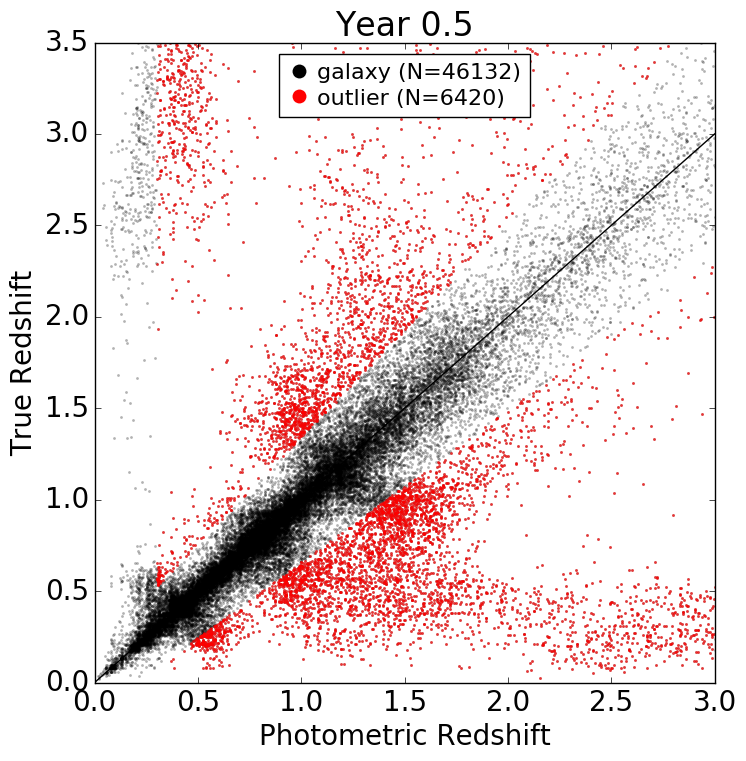
\includegraphics[width=5cm]{figs/photoz/pztz_nyears_p5.png}
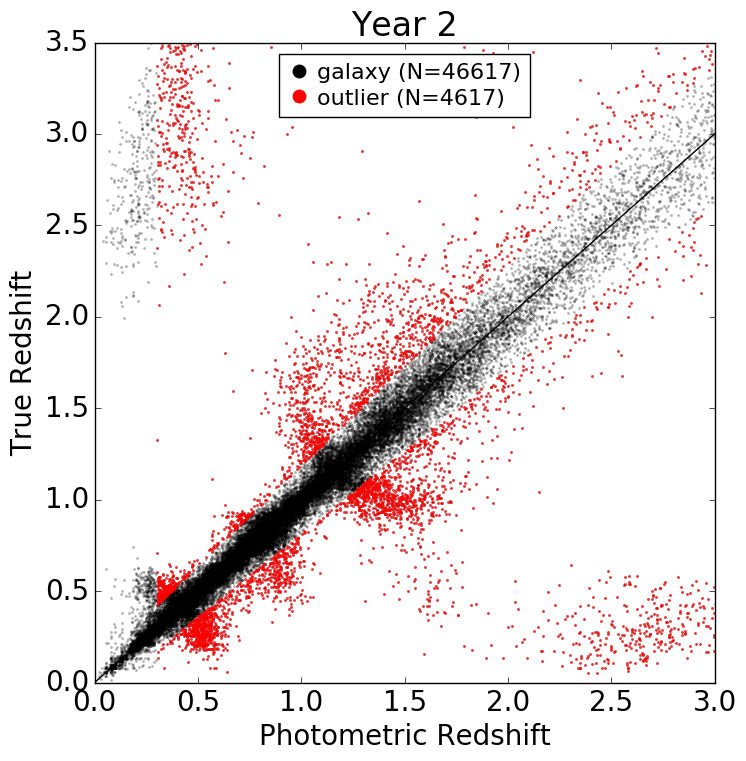
\includegraphics[width=5cm]{figs/photoz/pztz_nyears_2.png}
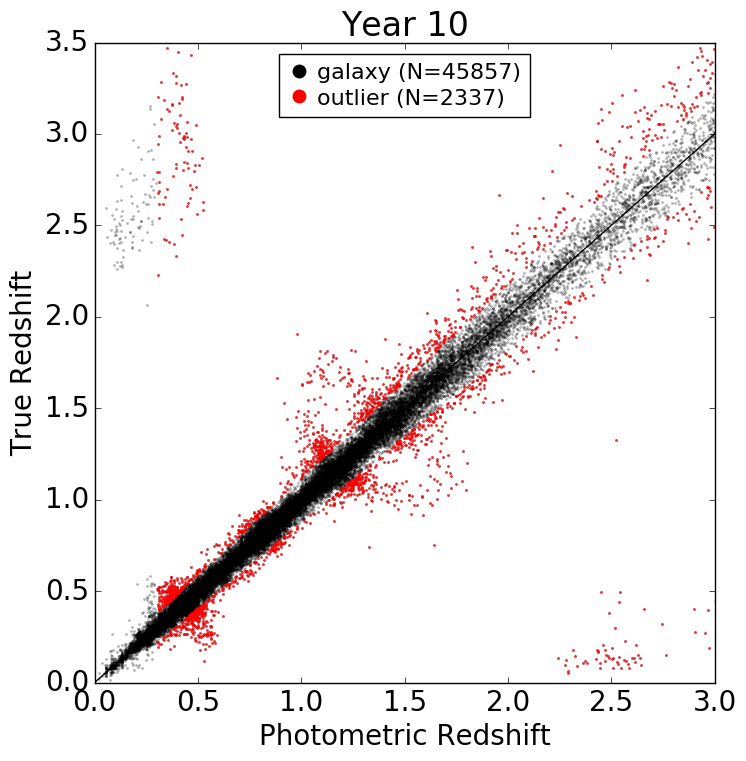
\includegraphics[width=5cm]{figs/photoz/pztz_nyears_10.png}
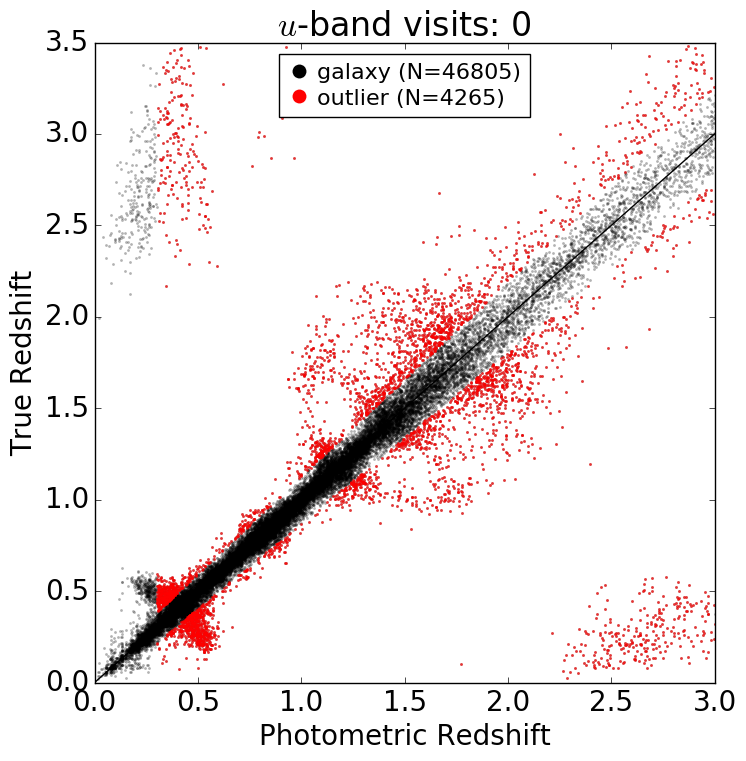
\includegraphics[width=5cm]{figs/photoz/pztz_uvisits_0.png}
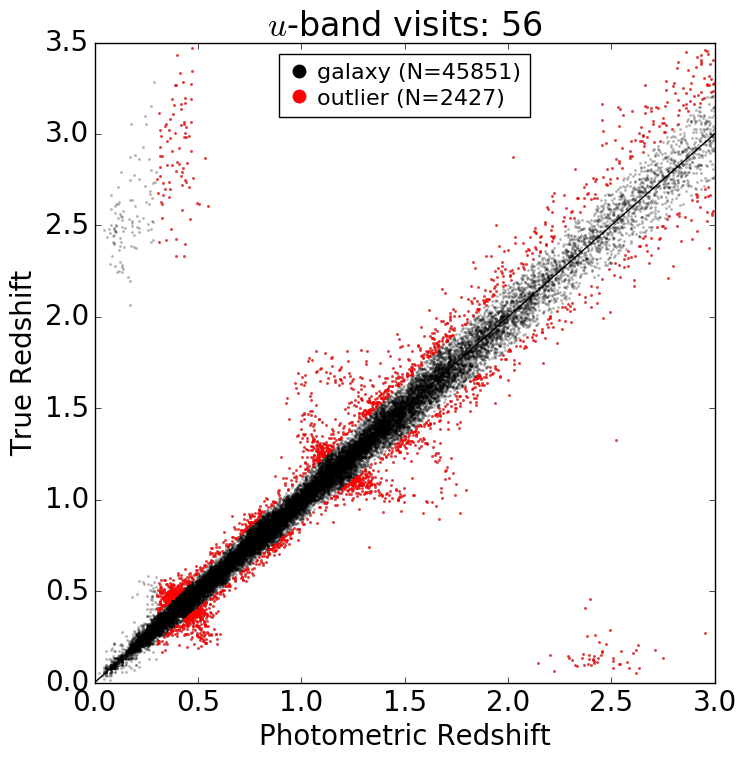
\includegraphics[width=5cm]{figs/photoz/pztz_uvisits_56.png}
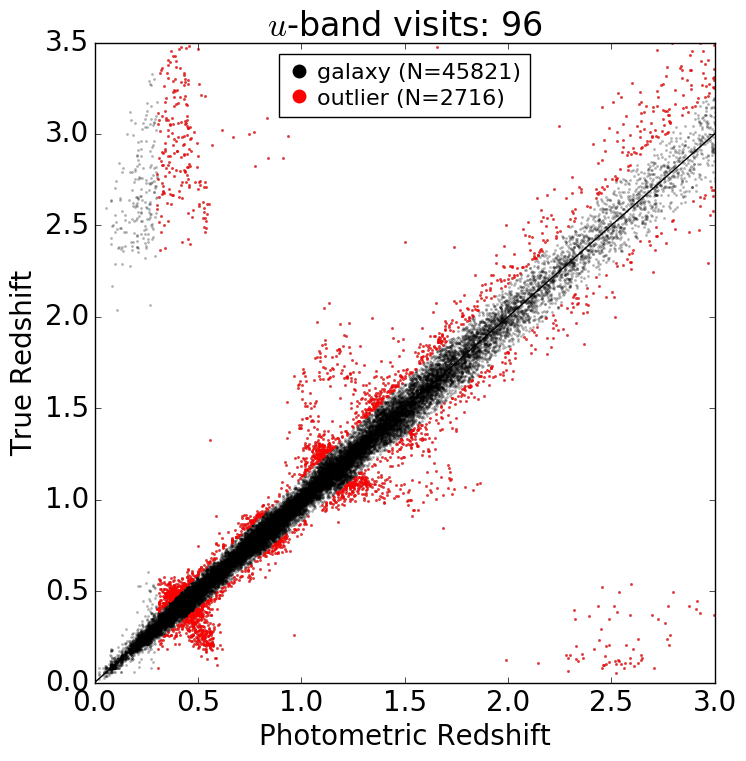
\includegraphics[width=5cm]{figs/photoz/pztz_uvisits_96.png}
\caption{Photometric vs. true (i.e., catalog) redshifts. Across the top row we show results from
0.5, 2.0 and 10.0 years of the LSST survey, and across the bottom row we show results for $0$,
$56$ (baseline), and $96$ $u$-band visits. 
\label{fig:redshifts}}
\end{center}
\end{figure}

\begin{figure}[h]
\begin{center}
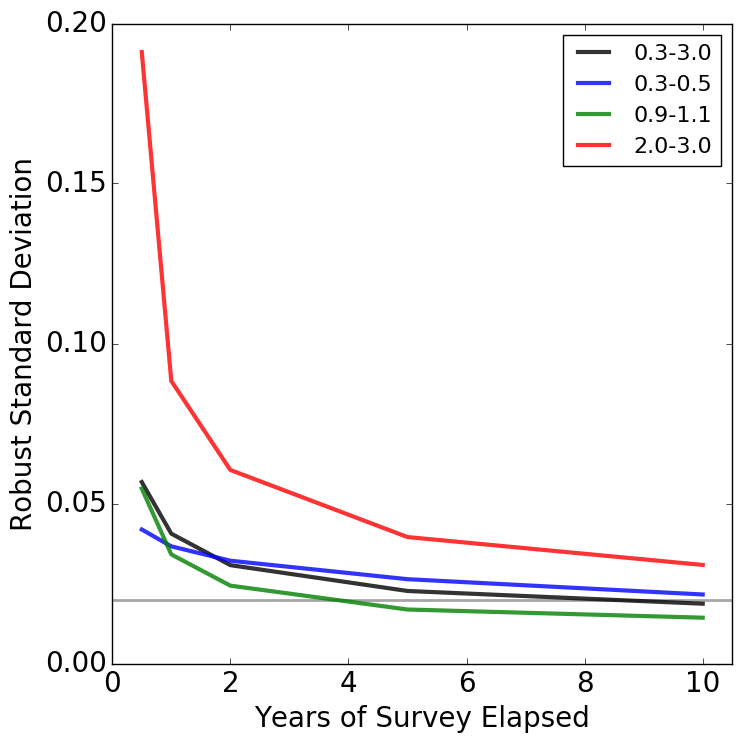
\includegraphics[width=5cm]{figs/photoz/pstat_nyears_IQRs.png}
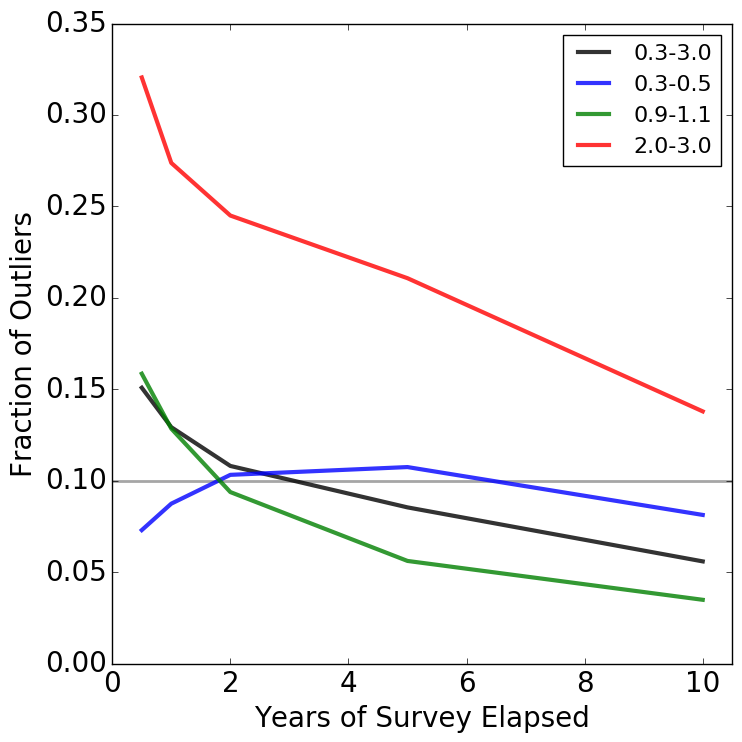
\includegraphics[width=5cm]{figs/photoz/pstat_nyears_fout.png}
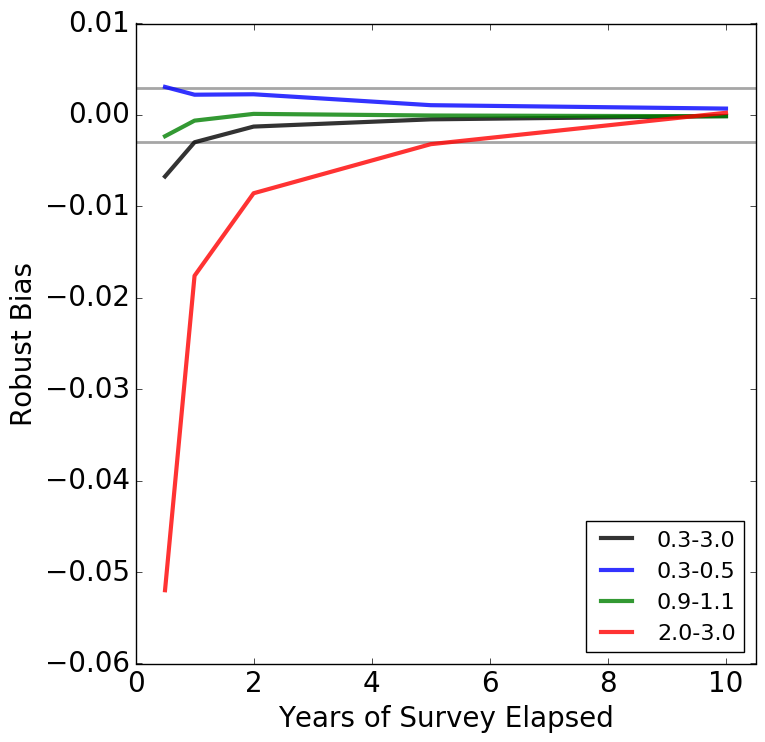
\includegraphics[width=5cm]{figs/photoz/pstat_nyears_bias.png}
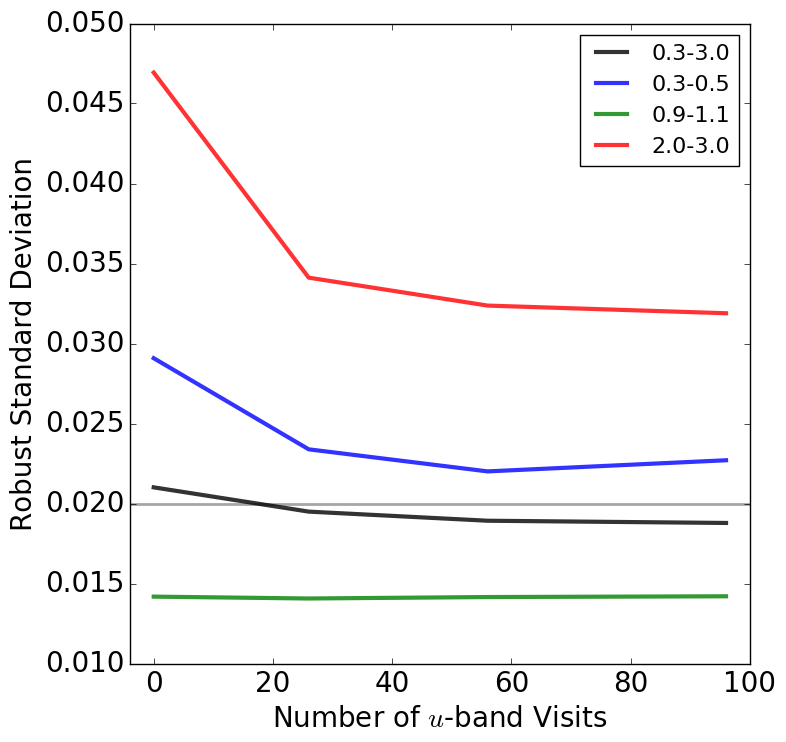
\includegraphics[width=5cm]{figs/photoz/pstat_uvisits_IQRs.png}
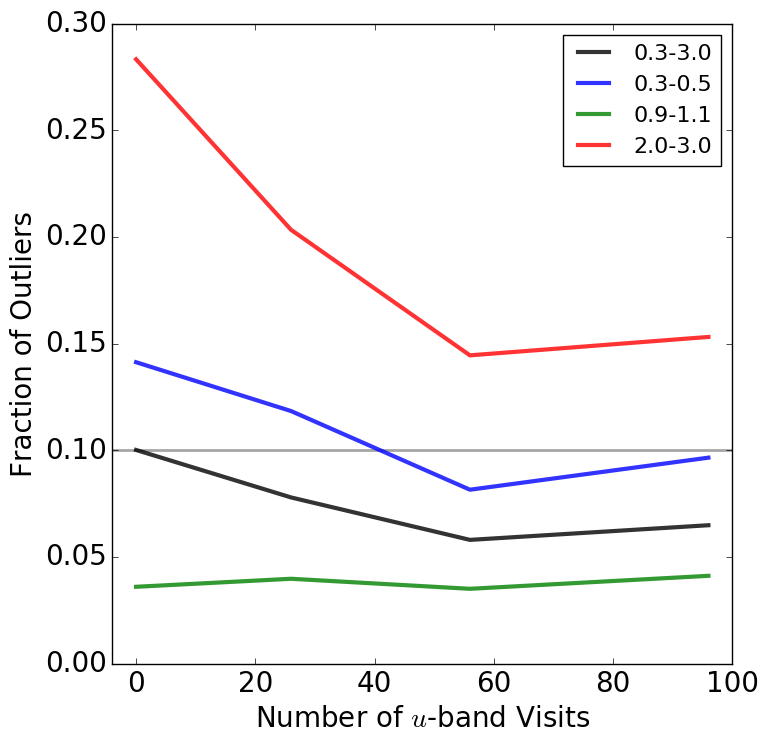
\includegraphics[width=5cm]{figs/photoz/pstat_uvisits_fout.png}
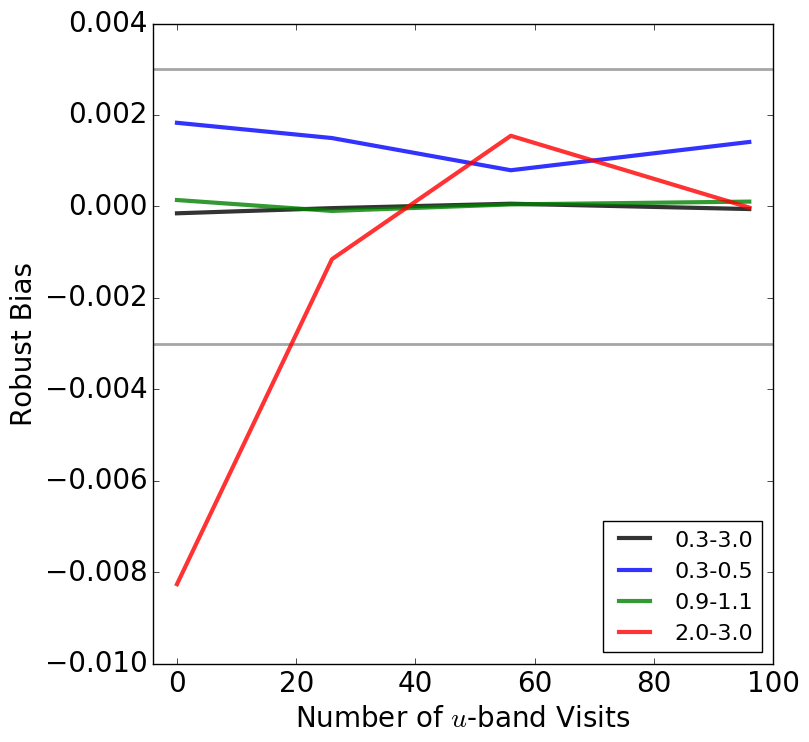
\includegraphics[width=5cm]{figs/photoz/pstat_uvisits_bias.png}
\caption{Three photo-$z$ metrics as a function of LSST parameters. From
left to right, the y-axis is the robust standard deviation, the fraction of
outliers, and the robus bias. The top row shows these statistics as a function
of the number of years of LSST survey, and the bottom row shows them as
a function of the number of $u$-band visits. Colors show these relations
for four bins in redshift: 0.3--3.0 (black), 0.3--0.5 (blue), 0.9--1.1
(green), and 2.0--3.0 (red). Grey lines mark the SRD specification for
each statistical measure.
\label{fig:metrics}}
\end{center}
\end{figure}


\subsection{Discussion}

\textbf{Additional considerations for observing strategy.} As mentioned
above, overall image depth and signal-to-noise is our primary concern,
so we are not testing changes in e.g., the inter-night gap time or the
exposure time of individual visits.  Our software is instead focused on
modifying other LSST parameters such as systematic offsets to the
magnitudes in each filter and/or coefficients for the magnitude
uncertainties in each filter in order to simulate improvements or
degradations the system throughput, sky background brightness, and other
such factors. We also aim to test airmass distributions (i.e., changes
to the effective filter functions), different progression rates for
filters (e.g., a scenario in which we complete all $u$-band by year 2),
scenarios in which some areas of sky have better/worse coverage at any
given time, and so forth. In all respects we are open to suggestions
from the community, and direct interested readers towards Graham et al. (2017; in prep.).
% Should be submitted by the end of May 2017, and then the reference can be updated.

\textbf{Considerations for building the real training catalog.} All
photometric redshift algorithms require training set data consisting of
objects with secure spectroscopic redshifts.  For LSST, many of these
will be contained in a small number of training/calibration fields (e.g.
COSMOS, VVDS).  Imaging these fields to full depth in all six bands
early in the survey (but under the range of observing conditions
expected for the ten year survey) will be key to characterizing
performance.  Inclusion of these patches of full-depth imaging must be
included in any cadence design. Future simulations of photo-$z$ results
can include varying the quality of the training catalog obtained by
LSST.

\textbf{Integration with MAF.} One way to extend our program to be able
to evaluate observing strategies simulated with \OpSim could be to use
the MAF to enable us to simulate representative samples of galaxies
across the mock LSST sky, and compute the metrics we have defined.
It may be possible to avoid such a large computation by first defining
some intermediate diagnostic metrics, such as the $u$-band coverage, and
working out how our higher level metrics depend on them, using some
approximate interpolation formulae.

\textbf{Connecting to the Dark Energy Figure of Merit.} The metrics we
have defined here should be able to be related to the DETF Figure of
Merit, but because photo-zs affect all of the LSS, WL and CL
cosmological probes, this step may need to wait until a joint
Figure of Merit MAF metric is developed.

% --------------------------------------------------------------------
%
 \subsection{Conclusions}

 Here we answer the ten questions posed in
 \autoref{sec:intro:evaluation:caseConclusions}:

 \begin{description}

 \item[Q1:] {\it Does the science case place any constraints on the
 tradeoff between the sky coverage and coadded depth? For example, should
 the sky coverage be maximized (to $\sim$30,000 deg$^2$, as e.g., in
 Pan-STARRS) or the number of detected galaxies (the current baseline but
 with 18,000 deg$^2$)?}

 \item[A1:] Since increasing the areal coverage comes at the expense of depth per pointing, this will adversely affect the photometric redshift quality. We estimate that only ~80\% of the galaxies would then meet the signal-to-noise threshold for photo-z analysis, but that this would be more than offset by the extra area and the final catalog would be ~108\% the size. Although this appears to be a net gain, it would change the redshift range for analysis.

 \item[Q2:] {\it Does the science case place any constraints on the
 tradeoff between uniformity of sampling and frequency of  sampling? For
 example, a rolling cadence can provide enhanced sample rates over a part
 of the survey or the entire survey for a designated time at the cost of
 reduced sample rate the rest of the time (while maintaining the nominal
 total visit counts).}

 \item[A2:] The sampling frequency is not important to photo-z, but building a uniform depth as a function of time would enable early science that relies on photo-z, so long as this depth is distributed across all filters. This distribution probably does not need to be exactly even, but tolerances have yet to be studied (e.g. rolling cadence may lead to seasonal variations that induce large-scale patchiness in the depth). However, sampling to full depth in all of the bands except g would have a negative impact, for example.

 \item[Q3:] {\it Does the science case place any constraints on the
 tradeoff between the single-visit depth and the number of visits
 (especially in the $u$-band where longer exposures would minimize the
 impact of the readout noise)?}

 \item[A3:] Photo-z would be improved if the u-band magnitude uncertainties could be further minimized, so long as this does not take away visits from other filters. If this could be done by longer u-band exposures during single-visits but less overall u-band visits, that would be good for photo-z.

 \item[Q4:] {\it Does the science case place any constraints on the
 Galactic plane coverage (spatial coverage, temporal sampling, visits per
 band)?}

 \item[A4:] Galactic plane coverage is not applicable to photo-z.

 \item[Q5:] {\it Does the science case place any constraints on the
 fraction of observing time allocated to each band?}

 \item[A5:] We find that at least ~20 u-band visits are necessary for the photo-z statistics to meet specifications.

 \item[Q6:] {\it Does the science case place any constraints on the
 cadence for deep drilling fields?}

 \item[A6:] Cadence of the DDF is not applicable to photo-z.

 \item[Q7:] {\it Assuming two visits per night, would the science case
 benefit if they are obtained in the same band or not?}

 \item[A7:] Intra-night filter changes do not affect photo-z.

 \item[Q8:] {\it Will the case science benefit from a special cadence
 prescription during commissioning or early in the survey, such as:
 acquiring a full 10-year count of visits for a small area (either in all
 the bands or in a  selected set); a greatly enhanced cadence for a small
 area?}

 \item[A8:] Photometric redshift analysis would be greatly assisted by acquiring a full 10-yr count of visits in all six bands for a small area during commissioning or early in the survey, especially if these assets are in regions covered by existing spectroscopic surveys.

 \item[Q9:] {\it Does the science case place any constraints on the
 sampling of observing conditions (e.g., seeing, dark sky, airmass),
 possibly as a function of band, etc.?}

 \item[A9:] Preliminary analysis shows that photometric redshifts may benefit by sampling in airmass, especially in the u-band, but a full assessment of the tradeoffs is pending. In general, a more uniform distribution of conditions is a guard against systematics.

 \item[Q10:] {\it Does the case have science drivers that would require
 real-time exposure time optimization to obtain nearly constant
 single-visit limiting depth?}

 \item[A10:] No

 \end{description}


\navigationbar

% ====================================================================


% --------------------------------------------------------------------

%+
% SECTION:
%    supernovacosmology.tex
%
% CHAPTER:
%    cosmology.tex
%
% ELEVATOR PITCH:
%    SNIa cosmology, approach to evaluating dependence of science on cadence
%
%-
% ====================================================================
\clearpage
\section{Supernova Cosmology and Physics}
\def\secname{supernovae}\label{sec:\secname}

\newcommand{\ml}[1]{\textcolor{red}{[{\bf ML}: #1]}}

Lead authors:
\credit{jhrlsst},
\credit{rbiswas4},
\credit{MichelleLochner}

Contributing authors:
\credit{sethdigel},
\credit{RobFirth},
\credit{astrofoley},
\credit{lgalbany},
\credit{pgris},
\credit{ReneeHlozek},
\credit{ivezic},
\credit{saurabhwjha},
\credit{RickKessler},
\credit{AlexGKim},
\credit{aimalz},
\credit{jasonmcewen},
\credit{janewman-pitt-edu},
\credit{hiranyapeiris},
\credit{kponder},
\credit{rlschuhmann},
\credit{astrostubbs},
\credit{msullivan318},
\credit{wmwv}

\subsection{Introduction}
The acceleration of the rate of expansion of the Universe at late times is one of the
most exciting and fundamental discoveries\citep{Riess1998,Perlmutter1999} in recent times.
This discovery was made using Type Ia supernovae (SNIa) as standardizable candles, and
implies that 76\% of the energy density of the Universe is composed of dark energy
\citep{Frieman2008}. Type Ia supernovae are believed to be explosions of white
dwarfs that have approached the Chandrasekhar mass and are disrupted by
thermonuclear fusion of carbon and oxygen.


This section is concerned with the detection and characterization of
supernovae (SNe) over time with LSST and their various scientific
applications. A crucial application is the use of SNIA %and potentially some core-collapse SNe
(like type IIP) to trace
to trace the recent expansion history of the universe, and confront models of the
physics driving the late time accelerated expansion of the universe.

LSST will improve on past surveys by observing a substantial number of well-characterized
supernovae, at high redshift. This large sample is not necessarily tied to the large area of LSST
and can rather be obtained from a relatively small spatial region, such as the Deep Drilling Fields
(DDF) with larger numbers of well-measured light curves due to the long time interval and high volume
at high redshifts.

On the other hand, the Wide-Fast-Deep (WFD) aspect will make the LSST survey
the first to scan a very large area of the sky for SNe. SNe that are detected
and well characterized by the WFD will provide 
\begin{itemize}
    \item a large, well-calibrated low redshift sample ($z \lesssim 0.1$) to replace/supplement the current  set of low redshift supernovae from a mixture of surveys. Such a large, clean low redshift sample is crucial in {\emph{providing a longer lever arm for the determination of cosmological parameters from supernovae.}}
    \item  a low and medium redshift ($z \lesssim 0.8$ and peaking at $z \sim 0.4$ ) spanning large areas of the sky and therefore with the ability of {\emph{tracing large scale structure}} in a novel way, particularly due to the inclusion of estimates radial distances. This will be possible by combining redshift estimates from supernova light curve in conjuncion with photometric redshifts from host galaxies.  Such a sample could also be used to probe the {\emph{isotropy of the late time universe.}}
    \item This large sample of SNe will also enable further sharpening of our understanding of the properties of the SN population of both Type Ia and core-collapse SNe (see \autoref{sec:transients:SNtransients}). Aside from the science described in \autoref{sec:transients:SNtransients}, this understanding will also be extremely important to the goal of SN cosmology from LSST. When selecting supernovae satisfying specific criteria from observations in magnitude limited surveys, a lack of understanding of the population properties leads to selection biases in SNIa cosmology as well as the steps in photometric classification~\cite{2017ApJ...836...56K,2016ApJ...822L..35S}. 
The WFD SN Ia
sample will dramatically increase the size of the sample available to
train such an empirical model, as well as understand the probability of
deviations and scatter from this model. Aside from issues like
calibration which need to be addressed separately, a larger sample of
such well measured SNe is probably the only way to address `systematics'
due to deviations from the empirical model. 
\end{itemize}
%The anticipated WFD sample can
%be thought of as consisting of two components:  the low-redshift sample
%which is more likely to be complete, and the higher-redshift sample that
%will be able to constrain evolution.

% --------------------------------------------------------------------

\subsection{Target measurements and discoveries}
\label{sec:\secname:targets}

SNe of different types are visible over time scales of about a few
weeks (e.g., type Ia) to nearly a year (type IIP).  During the full
ten-year survey, LSST will scan the entire southern sky repeatedly with
a WFD cadence, and certain specific locations of the sky called the Deep
Drilling Fields (DDF) with special enhanced cadence.

This spatio-temporal window should contain millions
of SNe. However, the actual sequence of
observations by LSST, defined by the series of field pointing as a
function of time in filter bands (along with weather conditions), and
conditions used for detection will determine the extent to which each
SN can be detected and characterized well.  Characterization of the SNe
is at the core of a number of science
programs that use them as bright, abundant objects with empirically
determined intrinsic brightnesses. While type IIP supernovae may prove to be useful standard
candles \citep{Sanders2014}, we will focus this work on the more well-established type Ia SNe.

Ultimately, the study of dark energy using LSST supernovae will be performed by an analysis inferring the parameters of a cosmological model using a sample of supernovae constructed from the LSST observations, and astrophysical models of supernovae that allow one to relate the peak intrinsic brightness to observed properties of the supernova. We should emphasize that while such analyses have been performed on previous SN surveys, the analyses that would be performed on a really large dataset would be different and is currently under study. Estimates of the potential of such surveys have often been measured using figures of merit such as the Dark Energy Task Force figure of merit~\citep{Albrecht2006}. The main goal of such a metric is to estimate the potential of a survey in elucidating the understanding of dark energy. However, our primary aim here is to study the relative impact that different LSST Observing strategies would have on such dark energy analysis, rather than absolute impact, and to communicate the characteristics of the survey that make a strategy better than others. This necessitates studying the quality of observations corresponding to typical individual supernovae or groups of supernovae rather than producing a single output for a survey. Therefore we identify some of the key steps in the supernova analysis which are directly related to observational characteristics of survey, and define metrics in terms of such quantities. In fact, these metrics should be  thought of as a total of scores, where these scores characterize the sequences of observation on small patches of the sky in small time windows. The key steps we have chosen are
\begin{enumerate}
\renewcommand{\theenumi}{\alph{enumi}}
\item The detection of SNe \label{it:detection}
\item Estimating the intrinsic peak brightness of a supernovae and its redshift
\item Photometric classification \label{it:typing}
\end{enumerate}
The efficacy of photometric typing, redshifts and estimation of intrinsic brightnesses
are all dependent on the amount of information available in the observed
light curves of SNe. While these steps are not necessarily independent, it
is useful to think of the requirements on some of these steps separately;
it is not unlikely  that combinations of some of the steps would still be
affected by similar requirements. Further, in the absence of a complete analysis, we opt for certain ad-hoc criteria in determining the threshold for such observations. This would be necessary even if we were to perform an analysis similar to past surveys.

{\emph{Supernova detection}}\\
Supernova light curves consisting of flux measurements at different times are built through photometry
at specific locations on each of the observed images. A finite list of such specific locations is
constructed through a transient detection pipeline studying difference images. In brief, this process
consists of studying subtractions between a  `template' image (coadded over time so that a supernova
flux averages to a small value) and single visit images called `science images` at different times,
after correcting for differences in resolution, observing conditions and pixel registration. In such
difference images, one expects to obtain non zero pixel values at locations of transients including
supernovae, and pixel values at other locations (including locations of static astrophysical
sources) to be
consistent with zero aside from a noise. The efficiency of detecting a supernova in a single
exposure
depends on a number of factors, the most significant of which is the signal (brightness of the supernova
in the science image compared to the template) to noise (SNR) in the relevant image.

%Thus, the probability
%of a supernova being detected in at least a fixed number of the images can be calculated from
%transients such as supernovae, with the probability of inferring the presence
%of an object with flux changing in these exposures being related to the change in
%brightness of the object and noise in the image. Combining a set of difference images
%along a supernova light curve results in higher probability of detecting a transient.

{\emph{Supernova classification}}\\
Because LSST will discover significantly more SNe than can be spectroscopically confirmed,
photometric classification of supernova type from multi-band light curves is crucial. While cosmology
with a photometric SNe sample with contamination from core collapse SNe is possible (see for
example 
\citet{Kunz2007,Newling2011,Hlozek2012,Knights2013,Bernstein2012,Gjergo2013,Campbell2013,Rubin2015,Jones2016})
,
these methods still benefit from accurate class probabilities from classification algorithms. To
investigate the effect of observing strategy on SNe classification, we use the multi-faceted machine
learning pipeline developed in \citet{Lochner2016}.


{\emph{Estimating intrinsic supernova brightness at peak}}\\
The ultimate goal of using SNe (type SN Ia or
SN IIP) for cosmology requires estimating the intrinsic brightness of each SN at peak. The first (and
sometimes only, depending on the light curve
model) step is fitting the calibrated fluxes to a light curve model with
a set of parameters. According to the ansatz used in SN cosmology, the
intrinsic brightness of SNe is largely determined by the parameters of
the light curve model; hence the uncertainties on the inferred
parameters largely determine the uncertainties on the inferred peak
intrinsic brightness or distance moduli of the SNe. This means the error on the fitted distance
modulus parameter is a useful proxy for the quality of the light curve and the accuracy of
the resulting cosmological inference.


% --------------------------------------------------------------------

\subsection{Metrics}
\label{sec:\secname:metrics}


Since the steps described above are all necessary for the determination of
SN intrinsic brightnesses, a metric for supernova cosmology must
quantify the ability to perform these steps on each supernova of the
sample. To connect this to the output of OpSim, we propose the
following strategy:
\begin{itemize}
    \item Study the sequences of observations in small spatial regions
    of the sky so that the sequences of observations relate to positions
    of astrophysical objects like supernovae. This capability is already
    built into \texttt{MAF} with multiple slicers like the
    \texttt{OpSimFieldSlicer} or the \texttt{Healpixslicer}. For example, in
    \autoref{fig:SN_sampling}, we show such a sequence for a WFD and
    DDF field for a single year.
    \item On each such spatial region, we look at sliding time windows,
    each time window of size about 70 days (corresponding roughly to a
    supernova Type Ia  lifetime starting 20 days before peak and
    extending to about 50 days after peak). As an example, we choose a
    time window around the night=570, which has an MJD value of 49923
    for both the fields (fieldID: 744 and 309) shown in
    \autoref{fig:SN_sampling} and show the time window in
    \autoref{fig:TimeWindow}.
    \item  We assign a metric value that we call \textbf{perSNMetric}
    $PM$ to each of these time windows to estimate the quality of
    observations for a supernova whose rough lifetime matches that time
    window. The prescription for assigning these values to each
    time window defines our metric and should quantify the success of
    the steps mentioned above. We would expect this value to be a
    function of the properties of the sequence of observations and the
    properties of the transients (SN) being studied. $$ PM =
    PM(\rm{observation Sequence, SN properties})$$
    \item We add up the \textbf{perSNMetric} for the time windows to
    estimate the metric values $M$ for the spatial region of the sky
    surveyed. $$M = \sum_i PM_i. $$ This gives us our final metric $M$.
\end{itemize}

\begin{figure}
 \centering
 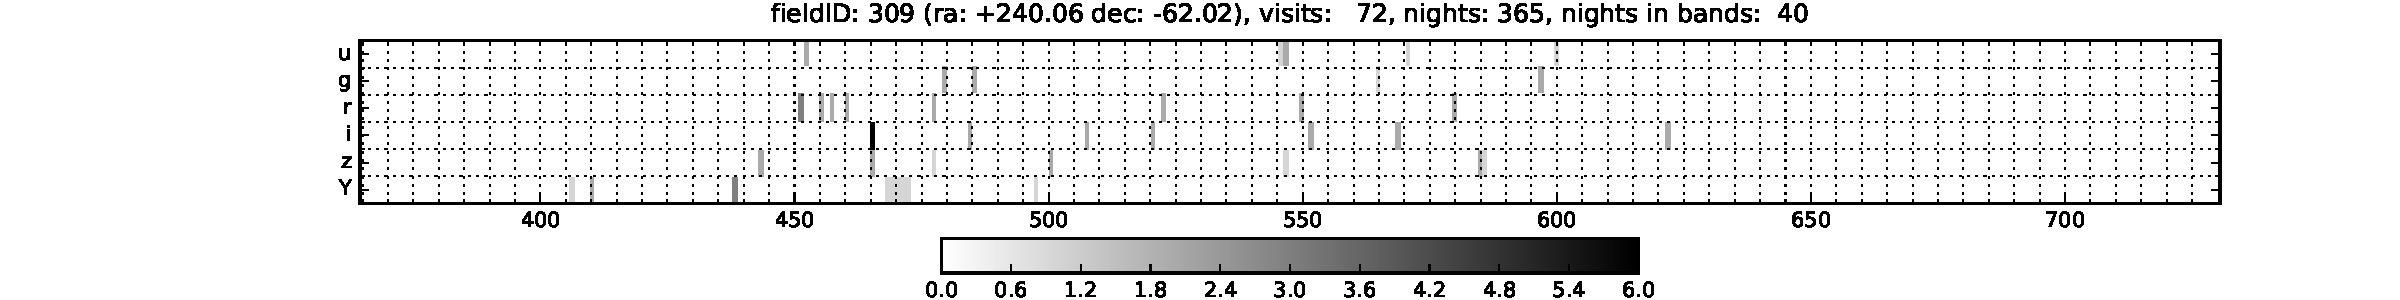
\includegraphics[width=\textwidth]{figs/supernova/fig_309_2ndYear}
 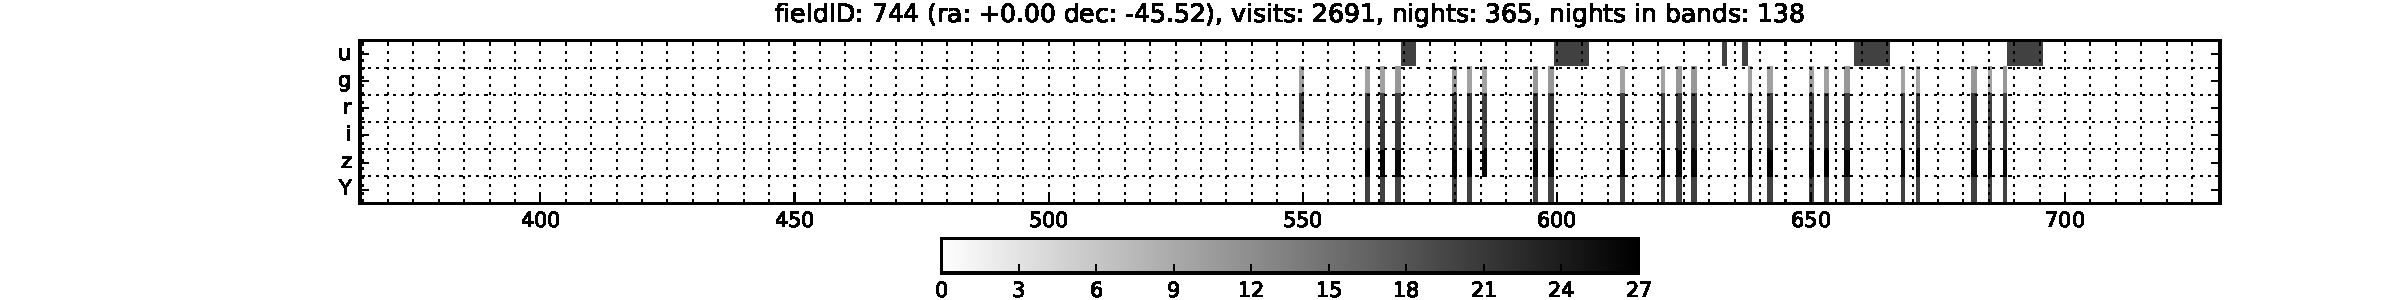
\includegraphics[width=\textwidth]{figs/supernova/fig_744_2ndYear}
 \includegraphics[height=0.2\textheight]{figs/supernova/loc_309_744.pdf}
 \caption{Example of the cadence in the 2nd season in a WFD Field
 (fieldID 309) (top-panel) and a Deep Drilling Field (fieldID 744)
 (middle panel) and the spatial location of these two fields shown on a
 map. The cadence plots show a heatmap of the number of observations per
 night during the second season in each filter u, g, r, i, z, y.
 The header shows the fieldID and location of
 the field, the total number of visits during that period, the number of
 distinct nights on which observations are taken, and the number of
 distinct observations (where observations are considered indistinct
 if they are on the same night and use the same band).}
  \label{fig:SN_sampling}
\end{figure}


\begin{figure}
\centering
 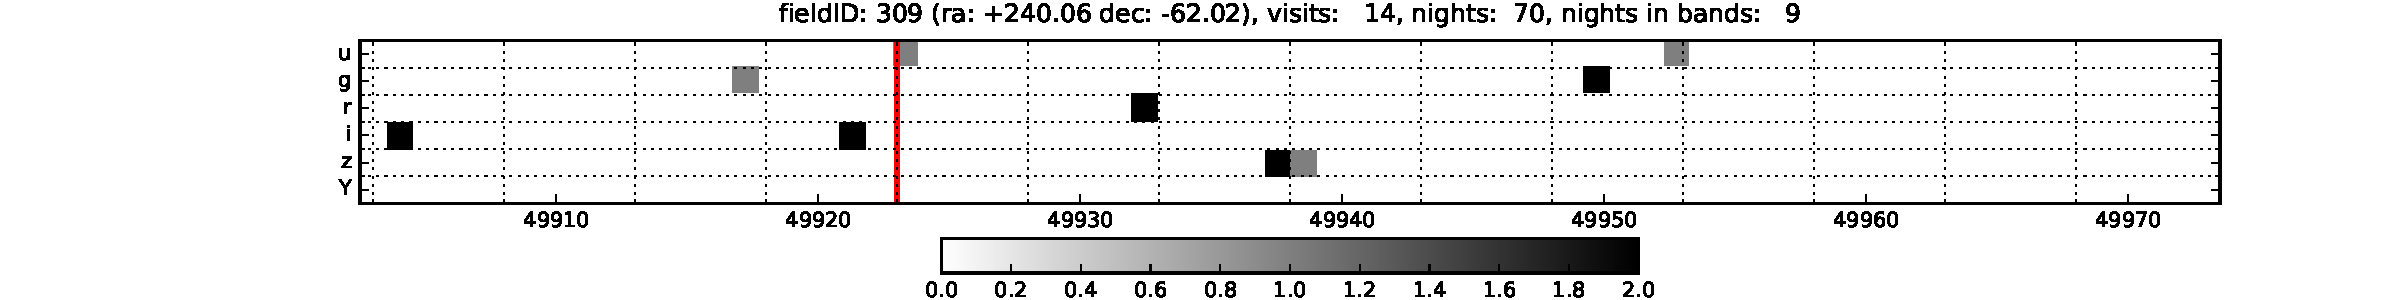
\includegraphics[width=\textwidth]{figs/supernova/TimeWindow_309_49923.pdf}
 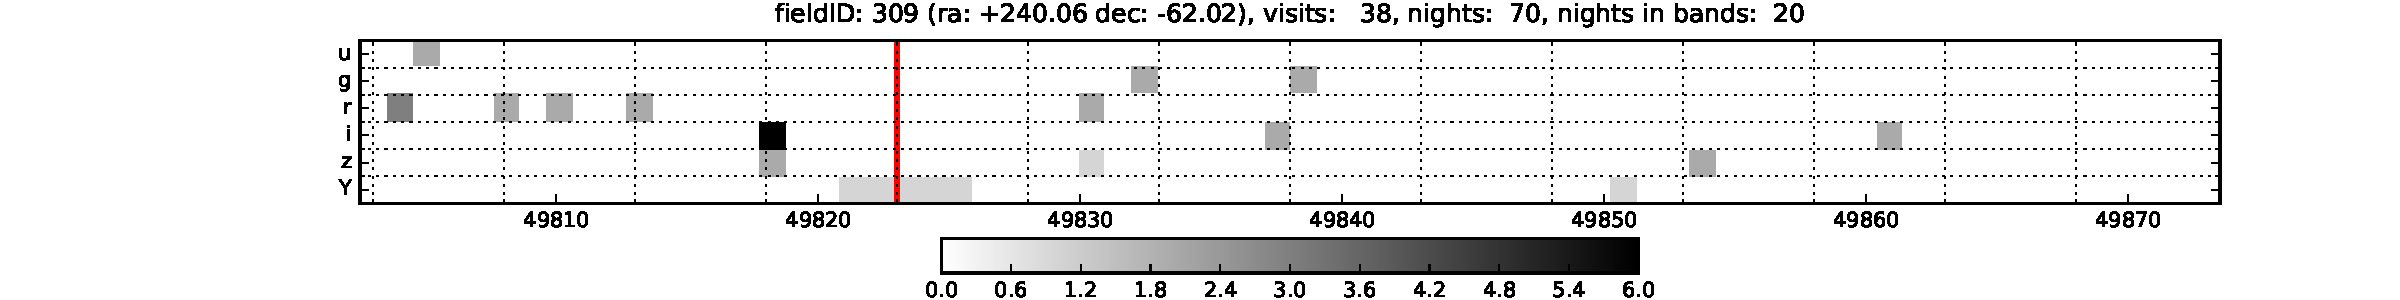
\includegraphics[width=\textwidth]{figs/supernova/TimeWindow_309_49823.pdf}
 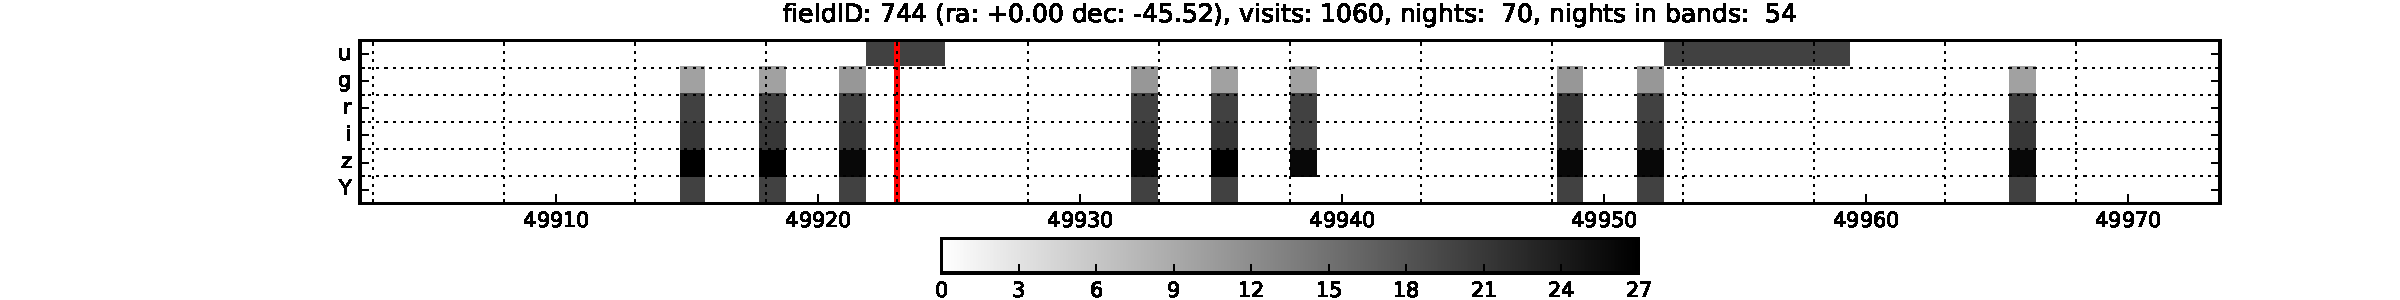
\includegraphics[width=\textwidth]{figs/supernova/TimeWindow_744_49923.pdf}
 %\includegraphics[height=0.2\textheight]{figs/supernova/loc_309_744.pdf}
 \caption{Example of a time window in a WFD Field (fieldID 309)
 (top-panel) and a second time window (middle panel) on the same field,
 and a Deep Drilling Field (fieldID 744) (bottom panel) all extending
 -20 days before and 50 days after a chosen night or MJD. For the Deep
 Drilling Field in the bottom panel, and the WFD field in the top
 panel, the chosen date around which the time window is constructed is
 the MJD of 49923, which is also 570 nights into the survey and marked
 by a red vertical line (which can be used to compare the location to
 \autoref{fig:SN_sampling}. The middle panel shows a window in Field
 309 centered around an MJD of 49823 or a night of 470 which may also be
 compared to \autoref{fig:SN_sampling}. The plots again show the
 heatmap of observations in each filter in each night as in the cadence
 plots of \autoref{fig:SN_sampling}.}
  \label{fig:TimeWindow}
\end{figure}

To define the metric $M,$ we need to define the perSNMetric. Two
different approaches to defining the perSNMetric for a given OpSim run are possible: a) Use
a simulated supernovae Type Ia with specific parameters, observed with
the sequence of observations in the above time window, and evaluate the
success of each step. b) Study heuristics of the observation sequences by using large simulations
with randomized parameter values. Here we will discuss the simpler approach (a).

%The SN metric in a spatial region
%reflects the contribution of the sample of SNe observed in that spatial
%region towards inferring the cosmological parameters. Let us
%consider a case where each SN observed with conditions better than a
%certain threshold contributes equally to the inference. Then the relevant
%metric would be a function of the number of SN in the sample passing
%such selection criteria. More generally, when the quality of all the
%supernovae are not similar, the metric should be thought of as
%the weighted sum of supernovae, with the weights being related to the
%inverse of the effective variance of the distance modulus:
%begin{equation}
%M\sim \sum_i w_i , \qquad  w_i \sim 1.0 /\sigma^2_\mu.
%\end{equation}
%By comparing with the form of the perSNMetric, we see that the
%perSNMetric should be a proxy for $1.0/\sigma^2_\mu,$ where
%$\sigma^2_\mu$ is the effective variance on the distance
%modulus of the supernova, as determined by fitting an empirical model to the supernova light curve.

%\subsubsection{ Steps in the PerSNMetric}
\subsubsection{Steps in the PerSNMetric}
\label{sec:persnmetric}
As described before, the measurement of the distance modulus is the
result of several steps. Therefore, we expect the perSNMetric to be a
product of metrics in each of the steps:

\begin{equation}
PM_i = \prod_{\rm{steps}} PM_i^{\rm{steps}}
\end{equation}

These components of perSNMetric constructed in different steps are
described in \autoref{tab:stepsAndMetrics}.
\begin{center}
 \begin{table}
\begin{tabular}{| p{5cm} |p{10cm}| }
\hline Metric & Description \\
\hline
I. SN discovery  (SNDM) &  Given the observations in a time window corresponding to the lifetime of
a supernova, evaluate the  probability of detecting a
transient. \\
II. SN classification (SNCM) & Given the observations in a time window corresponding to the
lifetime of a
supernova, evaluate the probability of accurately classifying the transient as a type Ia.\\
III. SN light curve characterization quality (SNQM) & Given the observations in a time window
corresponding to the lifetime of a supernova, evaluate the quality of characterization.\\
\hline
\end{tabular}
\caption{Components of the perSNMetric}
\label{tab:stepsAndMetrics}
\end{table}
\end{center}



\emph{I. Discovery Metric}

This metric is designed to gauge the performance of detection of SNe
discussed in \autoref{sec:\secname:targets}.
This metric is a proxy for the potential for a supernova to be detected
 during its lifetime by the set of images taken in different bands by LSST. The actual
 detection of SN during LSST is likely to use more stringent criteria, leading to 
 smaller numbers of supernovae in order to deal with possibly large numbers of false positives in detection. A larger
 number of images taken at a time when the supernova is bright enough increases the
 probability of detection. Technically, Assuming that a single detection in any of the images containing
 the supernova is sufficient to trigger photometry at the location, one can find the
 probability of detection from an SNR vs. efficiency of detection curve. The signal-to-noise ratio
(SNR) can be determined given properties of a supernova (redshift, intrinsic brightness etc.)
 and the five sigma depth provided in OpSim. While such a SNR-efficiency curve does not
 yet exist for the LSST pipeline, one can use such a curve from previous surveys, in particular a
 SNR-efficiency curve constructed during a stage of the Dark Energy Survey for g, r, i, z bands of DES
 \citep{Kessler2015}. This is shown in \autoref{fig:SNR_detection}.
\begin{figure}
 \centering
 \includegraphics[width=\textwidth]{figs/supernova/SNR_detection.pdf}
 \caption{Probability of detecting a transient from a single difference image in different bands as
a
 function of the signal-to-noise as obtained from Dark Energy Survey \citep{Kessler2015}. It shows,
that
for high SNR greater than $\sim 10,$ a single exposure used in difference imaging may be sufficient to detect the SN, while for
lower SNR, several such image differences may be necessary to have a high probability of
detection.}
 \label{fig:SNR_detection}
\end{figure}

Using this information, one can compute the value of the probability that a SN with given properties
will be discovered if from a set of images where the SN have a known signal to noise ratio. We use this as the
value for the supernova discovery metric (SNDM). While very high redshift (and thus faint)
supernovae will not be discovered, it is
potentially possible to discover many supernovae whose light curves will in turn not be well
characterized or hard to classify.


\emph{II. Classification Metric}

Separating supernovae from other detected transients is being considered in
\autoref{chp:transients}. Here we concern ourselves with problem of classifying subclasses of
SNe. Multiple techniques have been proposed to solve this problem \citep{Frieman2008,sako2008, kessler2010b, 
ishida2012, sako2014} and it is not yet clear how the
relative success of these techniques are affected by observing strategy. Work is ongoing to use the
multifaceted, machine learning pipeline developed in \citet{Lochner2016} to compare alternative
observing strategies. As this pipeline employs a variety of different feature extraction and machine learning
techniques, it is ideal to investigate the effect of observing strategy on the supernova classification. The exact 
metric used to determine the efficacy of the classification depends
on the exact problem at hand. For producing a general purpose, well-classified set of all types of
supernovae (for example, to study supernova population statistics), one could use the AUC metric
used in \citet{Lochner2016}, which is a good balance between purity and completeness. Ideally,
one would like a metric to be evaluated per object and included in the PerSNMetric. This is,
however, challenging as the success of classification will depend strongly on the nature of the
available training set, which will in turn depend on the spectroscopic follow-up program of LSST
and the availability of additional training data. Once a training set is determined and the
classification algorithm trained, a useful per-object metric is the classification probability of an
object being a Ia, which will be higher if the light curve is well-measured. This probability is
confounded by other factors (for example, other types appearing similar to Ia's), making
classification a very difficult metric to include on the per-object level. This is therefore left for future work.


\emph{III. Quality Metric}

We construct the quality metric for the perSNMetric by obtaining the
light curve of the SN in the time window described above. We fit the
light curve, using the SALT2 model \citep{Guy2007,2014A&A...568A..22B}, and approximately estimate the uncertainty in
distance from
the light curve fit alone. Of course, as is well known, luminosity
distance estimates of supernova Type Ia also show an intrinsic scatter
of around $0.1$ in previous surveys, which may be expected to decrease
with better training samples and understanding of underlying
correlations of SN Ia properties and their environments. We compute a
quality metric for each SN Ia as the ratio of the square of the
intrinsic dispersion to variance of the distance indicator from the supernova. 
$$ QM = 0.05^2/\sigma^2_{\mu}.$$ If our sample had a perfect discovery rate, and good classification (for example if we had spectroscopic classification), the uncertainty on
cosmological parameters would be entirely due to this quality metric and would be expected to scale with the quality metric as 
$$\frac{1}{\sigma} \sim \sqrt{\sum{\frac{1.0}{1.0 + 1.0 / QM}}}$$
where the sum is over the SNe in the sample.

%Move this to OpSim analysis
% The quality metric evaluated on the example SN plotted is $1.0$ if observed in the deep field
% (\autoref{fig:SNIaLCopsimdeep}), and $0.002$ in the WFD field (\autoref{fig:SNIaLCopsimmain}).



% --------------------------------------------------------------------

\subsection{OpSim Analysis}
\label{sec:\secname:analysis}
The scientific goal of characterizing SNe is, to a large extent, dependent
on how well the light curves of individual SNe are sampled in time and
filters. To study this, we re-index the OpSim output on spatial
locations rather than use the temporal index. Here, we first illustrate
in terms the cadence in two example LSST fields.

% {\bf Analysis, Results and Discussion}


% \begin{figure}[tbh!]
% %\vskip -1.3in
% \includegraphics[angle=0,width=0.99\hsize:,clip]{figs/SN_309_lcavg.pdf}
% %\vskip -1.3in
% \caption{Time-interval averaged light curve of
% \autoref{fig:SNIaLCopsimmain}. The light curve shows only a small number
% of the data points, which is insufficient to classify this object as a
% Type Ia and may be also difficult to classify this object as a SN. }
% \label{fig:SNIaLCopsimmain2}
% \end{figure}







% \begin{figure*}[!hb]
%     \begin{minipage}[b]{\linewidth}
%         \includegraphics[width=\textwidth]{figs/supernova/fig_firstSeason_0}
%         \includegraphics[width=\textwidth]{figs/supernova/fig_firstSeason_1}
%         \includegraphics[width=\textwidth]{figs/supernova/fig_firstSeason_2}
%         \includegraphics[width=\textwidth]{figs/supernova/fig_firstSeason_3}
%         \includegraphics[width=\textwidth]{figs/supernova/fig_firstSeason_4}
%     \end{minipage}
% \label{fig:opsimSummary}
% \caption{Cadence of Observations in the timewindow of a year towards a few sample of
% positions. Grey-scale indicates the number of visits. {\it add details}
% }
% \end{figure*}


We analyzed the OpSim output of the Baseline Observing Strategy,
enigma$\_$1189$\_$sqlite.db{\footnote
{\url{http://ops2.tuc.noao.edu/runs/}}} which includes Deep Drilling
Fields (DDF) and the main survey (WFD). While this is no longer the current baseline observing
strategy, we do not anticipate our conclusions would change with the use of
\texttt{minion\_1016}. Future work will include repeating our analyses with new OpSim runs, such as
\texttt{kraken\_1043}, which does not enforce visit pairs, and the new experimental rolling
cadences.

Using the OpSim output \texttt{enigma\_1189}, we generated
light curves for a type Ia supernova with a with a redshift of z=0.5 at a few different
locations. A date in MJD is chosen where the LSST simulated data are
reasonably well populated. We used the SALT2-extended model
with $x_0$, $x_1$ and $c$ set so that the SN Ia would have a specific
magnitude of $-19.3$ in the rest frame BessellB band. This was performed
using a version of \texttt{SNCosmo} to interpolate the SALT2 surfaces, and the
LSST catalog simulation package to calculate the flux for LSST
bandpasses.


\autoref{fig:SNIaLCopsimdeep} shows the light curve in
different filters in a deep drilling field. The
number of visits for 50 days (which is the period of the simulated SN Ia light curve in
rest-frame, which translates to 75 days at z=0.5) is 53 per filter. For this light
curves, the supernova quality metric (SNQM) and the
discovery metric (SNDM), are both equal to 1. SNDM=1 indicates that this object is a transient that
will be definitely discovered, and SNQM=1 indicates that the light
curves will be of high quality enough to contribute extremely well to
the inference of cosmological parameters. The light curves and
quantified metric demonstrate that data from Deep Drilling Fields would
generate high quality light curves, allowing a high rate of supernova
discovery.

In contrast, \autoref{fig:SNIaLCopsimmain} shows a light curve from the WFD survey. This light
curve is
generated in Field 290 and has an average number
of data points in the light curve of 2 per filter. Using these light
curves, the probability (SNDM) of detecting this supernova is less
than 0.1. \autoref{fig:perSNCadence} directly compares the light curves and cadences of the two
fields considered, from the DDF and WFD.

\begin{figure}
%\vskip -1.3in
%*\includegraphics[angle=0,width=0.99\hsize:,clip]{figs/SN_290_lc.pdf}
\centering
\includegraphics[angle=0,width=14truecm]{figs/supernova/SN_290_lc.pdf}
%\vskip -1.3in
\caption{An example of a light curve, in six filter bands, of a SN Ia from the DDF field with fieldID 290 in
\texttt{enigma\_1189}.
}
\label{fig:SNIaLCopsimdeep}
\end{figure}

\begin{figure}
%\vskip -1.3in
\centering
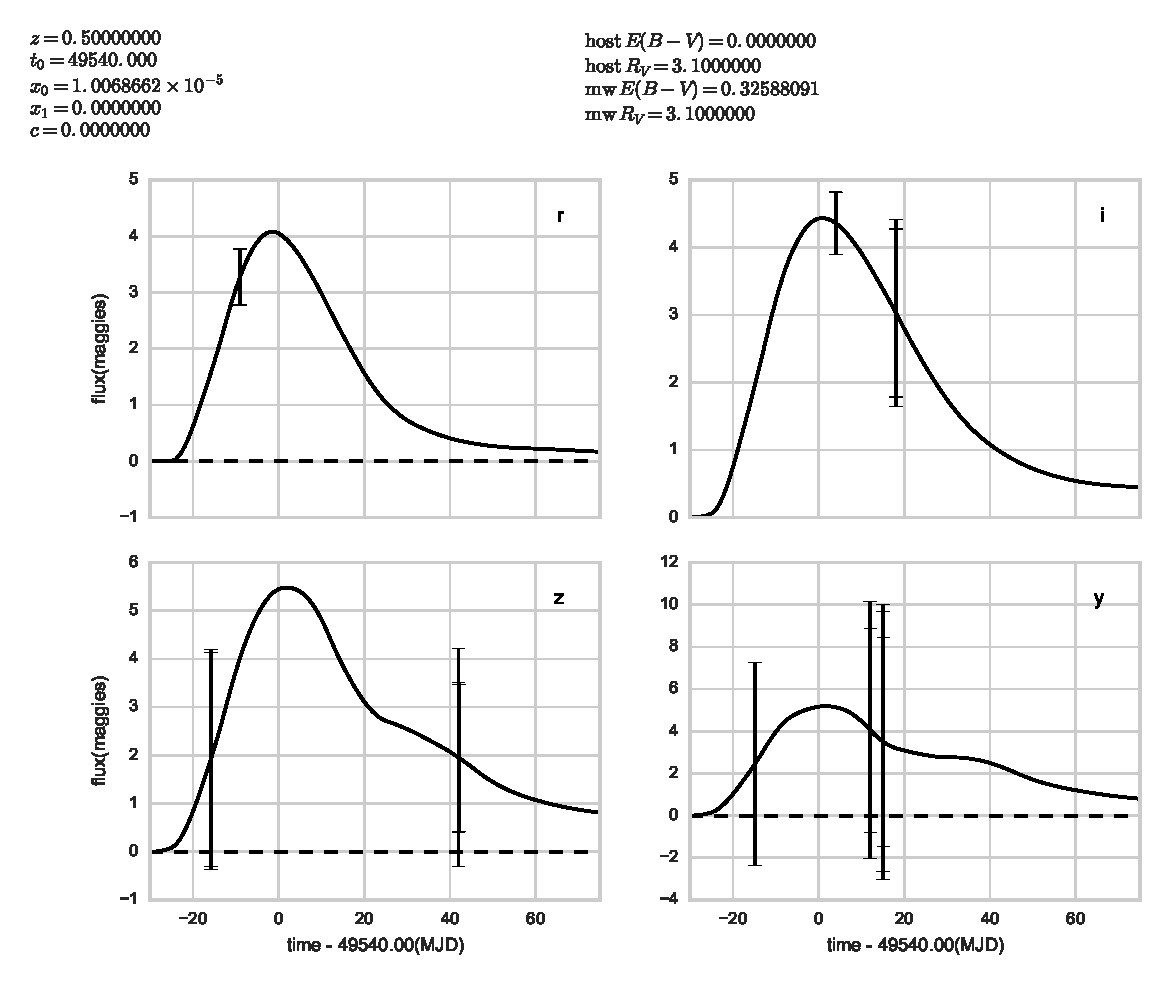
\includegraphics[angle=0,width=0.99\hsize:,clip]{figs/supernova/SN_309_lc.pdf}
%\vskip -1.3in
\caption{An example of a light curve, where only four filter bands are available, of a SN Ia from
the WFD survey in
\texttt{enigma\_1189}.
}
\label{fig:SNIaLCopsimmain}
\end{figure}

\begin{figure}
\centering
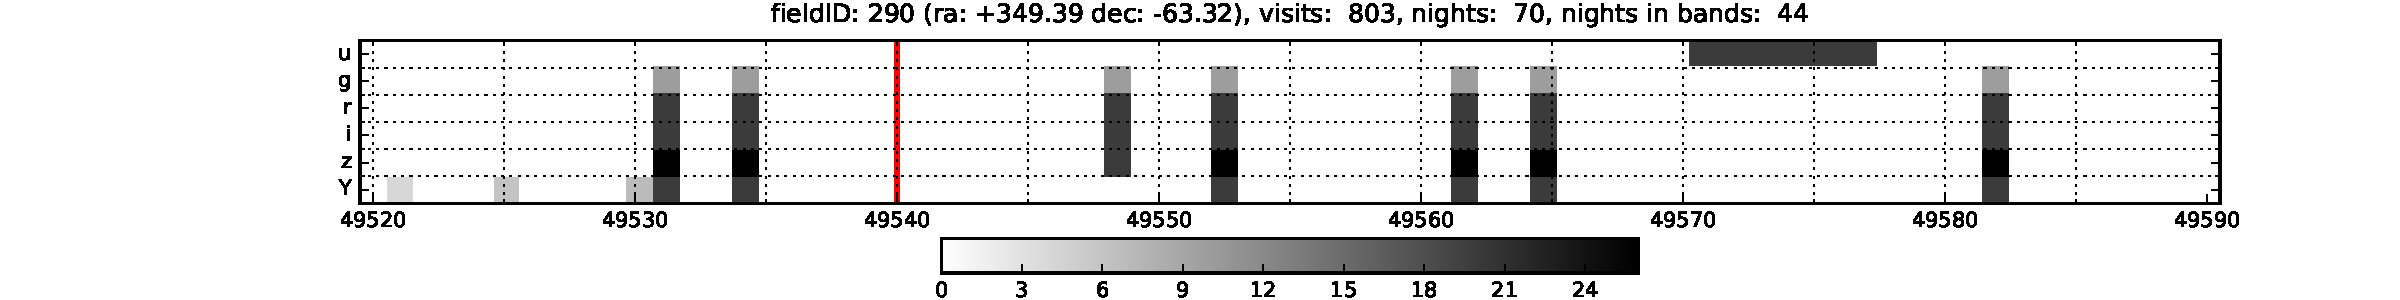
\includegraphics[angle=0,width=\textwidth,clip]{figs/supernova/SN_Cadence_290.pdf}
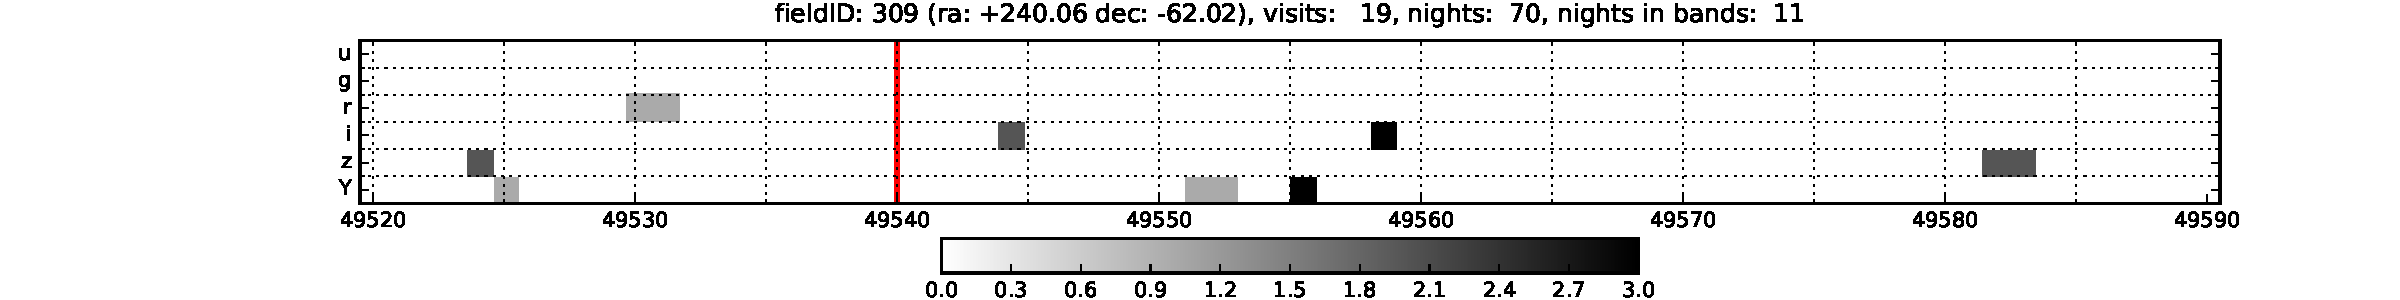
\includegraphics[angle=0,width=\textwidth,clip]{figs/supernova/SN_Cadence_309.pdf}
\caption{Cadence of observations in the time window of a representative
supernova at redshift of $z=0.5$ in a DDF (top) field (fieldID: 290) and
a WFD (bottom) field (fieldID: 309). The red lines show the date of
peak, and the shades show the number of observations in a night in
a distinct filter.}
\label{fig:perSNCadence}
\end{figure}

{\bf Analysis Results:}
To further study the quality of light curves across the survey, we simulate the same type Ia
supernova in 16 different fields, including DDF 290 already studied, from the \texttt{enigma\_1189}
OpSim run and record the average number of visits per 50 day time window
(\autoref{tab:lcpositions}). A well-known rule of thumb (R. Foley, priv. communication) for good
quality SN light curves is to
demand 7-10 epochs per light curve spread over 50 days or so for more than one filter.
\autoref{tab:lcpositions} list characteristics of light curves towards 15 fields in the OpSim
output.

We summarize results of light curve analysis using OpSim output as follows:
\begin{itemize}
\item A high portion of the light curves, in both the WFD and DDF, can be identified as transients
using  the SN
discovery metric (SNDM$>$0.5 in \autoref{tab:lcpositions}).
This metric is currently using SNR of detections.
\item Light curves from WFD show poor qualities (SNQM$<$0.3) whereas the light curves from DDF show
high quality ($\geq$1). Note that we examined only a few cases of SNe at redshift of 0.5 and the
metric will be applied to a much larger range of SNe in future simulations.
\item We have explored ways to improve SN classification \citep{Lochner2016} and the classification
metric is described in Section
\ref{sec:\secname:metrics}.
In this analysis, we have not yet considered classification based on individual light curves.
This is because, unlike the discovery and quality metric, it is difficult to discuss
classification of a single object without having a well-defined training set, which is yet to be
determined for LSST.
\item In conclusion, based on the SNQM, we have showed that WFD data alone using the Baseline
Observing Strategy are not useful for SN studies.
\end{itemize}


%Although
%the averages in \autoref{tab:lcpositions} are only approximations because the cadence is
%non-uniform, they give a clear indication that with the \texttt{enigma\_1189} observing strategy,
%the WFD will not be useful for SNe studies.

{\bf Need for LSST observing strategy optimization for SN science:}

The results from our OpSim analysis motivate our proposal of a rolling cadence
in order to improve the sampling of SNe over a much larger area than the DDFs.
The DDF are useful for SNe at redshifts between 0.6 and 1.2, and the WFD will help us to increase
the number of SNe at low redshift
as shown in Figure 11.1 of LSST science book \citep{2009arXiv0912.0201L}. For example, a higher
number of SNe at z $=0.4$ is expected from WFD than DDF.
Consequently, DDF will have only a few SNe at low redshift,
since the DDF sample is limited to small patches of sky.
A significant scatter in distance modulus of low redshift SNe is found \citep[e.g.][]{Suzuki2012} which hinders deriving accurate
cosmological parameters.
Since the cosmology measurement requires low as well as high redshift distance moduli, a large
sample
of low redshift SNe will improve the cosmological parameter inference. The WFD would also provide a
useful sample of nearby supernovae to better constrain variations in SNe populations (for both
type Ia and core-collapse SNe).
Light curves from WFD
with reasonable quality can be achieved using our new proposed
observing strategy.

A larger sample of well-characterized light curves from the WFD can address two key science
goals:
\begin{itemize}
\item Tightly constraining cosmological parameters ($\Omega_M$ and $\Omega_\Lambda$)
by improving the measurement of distance modulus of low redshifted SNe. Without implementing
the new observing strategy that we recommend below, LSST will not be able to
make a significant contribution to SN cosmology below z$<$0.5.
\item The WFD offers a unique opportunity for isotropy studies (complementary to large-scale galaxy
surveys) and dynamical dark energy studies. Apparent luminosities and number counts can be
estimated for a large range of angular scales and
redshifts with WFD. However, this science case will only be possible with a large sample of
well-characterized SN Ia in a large field of view, providing further support for our
recommendation of a rolling cadence observing strategy.
\end{itemize}



% [ML] I've removed this (fairly arbitrary) chategorization, it's more confusing than helpful
% and it's clear how bad WFD is from the numbers alone

% In column 5, we categorize the positions into 5 categories
% base on the data points (the value in column 3) per filter for 50 days.
% When the number of LSST data points (the value in column 3) per filter
% for 50 days is $>$9 as the category A, 5-9 as B, 1.8 -- 5 for C, 1 --
% 1.8 for D, and $<$1 for E. An example of light curve of Category A has
% been shown in Figure \ref{fig:SNIaLCopsimdeep}, Examples light curves of
% Category B have been shown in Figures \ref{fig:SNIaLCopsimmain} and
% \ref{fig:SNIaLCopsimmain2}, respectively. An example of a light curve of
% Category C (ex. Dec.=-40 ;No. 7 in Table \ref{tab:lcpositions}) is shown
% in \autoref{fig:SNIaLCminus40}.

% \new{An example of Category B toward -66$^{\circ}$ is shown
% \autoref{fig:SNIaLCminus66} (No. 3 in \autoref{tab:lcpositions}). The
% light curves in {\it u, g} and {\it r} bands have 3 -- 5 data points,
% while {\it i} band has 8 or more than data points. The band z and y show
% relatively large error bars. In order to increase probability to
% recognize the light curve as a SN and Type Ia, simulated LSST data
% points could be increased by a factor of 2-3. Our goal is to improve the
% light curves which belong to Category B and C so that we can distinguish
% them as a SN and particularly as a Type Ia SN. This will improve values
% in SNDM and SNQM.}

\begin{center}
\begin{table}
%\tabletypesize{\scriptsize}
\centering
\begin{tabular}{|p{1.3cm} |p{3.3cm}|p{4cm}|p{1.9cm}|p{1.7cm}|p{1.7cm}|}
%\begin{tabular}{|p{0.9cm} |p{3.3cm}|p{4cm}|p{1.9cm}|}
\hline
 FieldID & (R.A., Decl.) & Number of LSST visits per year (u,g,r,i,z,y)       & Number of Avg. data
per SN period per filter & SNDM  & SNQM\\
\hline
290 DDF  & (349.386,-63.321)  & 2363 (398,229,402,414, 522,396) & 53 & 1.0  & 1.6 \\
 17      & (190,-83) &    239 (38,41,41,44,33,42) & 5.3 & .. & ..\\
% 290  &(20,-83) & 252 (52,56,40,21,37,44)  &5.7 &&\\
 22      &(20,-83) & 252 (52,56,40,21,37,44)  &5.7 &..&..\\
%old 3      &(120.012,-71.879) &  220(36,38,37,32,44,33) & 5.0 & B &\\
  217      &(116,-66) &  220 (36,38,37,32,44,33) & 5.0  & .. & ..\\
% 290(+DDF)  &(116,-66) &  220 (36,38,37,32,44,33) & 5.0  && 1.0 & 8.28\\
 309      &(240.05,-62.02) &101 (2,5,11,19,19,45) & 2.2 & 1.00 & 0.10  \\
 645      &(120,-50)  &80 (4,7,9,18,24,18)        & 1.8 &0.54 & 0.01\\
 949      & (80,-40)  &      96 (5,8,15,17,27,24) &  2.2 & 0.99 & 0.09\\
 948      & (280,-40) &      86 (4,2,6,4,24,18)   &  2.0 & 0.99 & $<$0.002\\
 1401      & (58,-27)   & 98 (3,3,9,26,31,26) &   2.2 & 0.77 & 0.002\\
 1754      & (30,-20)  &      86 (3,4,10,21,27,21) &  2.0 & 1.00 & 0.05\\
 1720      & (100,-20) &      58 (4,2,6,4,24,18)   &  1.3 & 0.99 & 0.03 \\
% 000  & (358.41,+0.18)  &                      &     & C({\it 0.1}) & \ref{fig:SNIaLCDecp18}\\
 2556  & (6.097, -1.105) & 80 (4,7,9,18,24,18)  & 1.8 & 1.00 & 0.05\\
% 290  & (6.097, -1.105) &                      &     & C({\it 0.1}) & \ref{fig:SNIaLCDecp18}\\
 2718     & (50,+1.5) &      72 (3,6,10,12,22,19) &  1.6 & 1.00 & 0.09\\
 2751     & (320, +5) &      7 (0,0,2,0,4,0)      &  0.2 & 0.09 & 0.02\\
% 2910     & (60,+5)   &      66 (0,7,11,20,28,0)  &  1.5 &.. & ..&\\
 3606     & (60,+20)  &      72 (0,8,13,22,29,0)  &  1.6 &..& ..\\
% 3959     & (60,+30)  &      44 (0,5,6,15,18,0)   &  1.0 &&\\
\hline
\end{tabular}
\caption{Table of 15 fields in the OpSim run \texttt{enigma\_1189}. The first column is simply an
index, with the special example fields of the DDF field 290 indicated. The
position of the fields is shown in column 2. The third column contains the total and per filter
band number of visits per year and this is averaged per filter per 50 day time window in column 4.
It can be seen that with this observing strategy, only the deep drilling fields are suitable for
supernova cosmology, where 7-9 data points per filter band is considered adequate quality. SNDM and
SNQM are SN discovery and quality metric, respectively, in the last two columns. Note that the
metric measurements are missing for some entries due to a spatial mismatch in fields that will be
rectified in future.}
\label{tab:lcpositions}
\end{table}
\end{center}

% \begin{center}
% \begin{table}
% %\tabletypesize{\scriptsize}
% \begin{tabular}{|p{0.7cm} |p{2.8cm}|p{4cm}|p{1.7cm}|p{1.4cm}|p{0.7cm}|}
% \hline
%  Field or No. & (RA,Dec) & No. of LSST data per year (u,g,r,i,z,y)       & Avg. No.&Category (TPR)
% &Fig. No. \\
% % Field or [No.] & (RA,Dec) & No. of LSST data per year (u,g,r,i,z,y)       & Avg. No. per filter
% per 50 days   &Category (TPR)\\
% %  or No.      &  (J2000)  & per year (u,g,r,i,z,y) & per filter & (TPR)    \\
% %        &           &                        & per 50days &     \\
% 290 DDF  & (349.386,-63.321)  & 2363(398,229,402,414, 522,396) & 53 &
% A(1)&\ref{fig:SNIaLCopsimdeep}
%  \\
%  1      & (190,-83) &    239(38,41,41,44,33,42) & 5.3 & B ({\it 0.4}) & \\
%  2      &(20,-83) & 252(52,56,40,21,37,44)  &5.7  & B  & \\
% %old 3      &(120.012,-71.879) &  220(36,38,37,32,44,33) & 5.0 & B &\\
% 3      &(116,-66) &  {\it 220(36,38,37,32,44,33)} & 5.0 & B & \ref{fig:SNIaLCminus66} \\
%  4      &(240.05,-62.02) &101(2,5,11,19,19,45) & 2.2  & B & \ref{fig:SNIaLCopsimmain2}\\
%  5      &(120,-50)  &80(4,7,9,18,24,18)        & 1.8 &  C &\\
%  6      & (80,-40)  &      96(5,8,15,17,27,24) &  2.2 & C &\\
%  7      & (280,-40) &      86(4,2,6,4,24,18)   &  2.0& C &\\
%  8      & (30,-20)  &      86(3,4,10,21,27,21) &  1.96& C & \\
%  9      & (100,-20) &      58(4,2,6,4,24,18)   &  1.3& D &\\
% % 000  & (358.41,+0.18)  &                      &     & C({\it 0.1}) & \ref{fig:SNIaLCDecp18}\\
%  309  & (6.097, -1.105) & 80 (4,7,9,18,24,18)  & 1.83   & C({\it 0.1}) & \ref{fig:SNIaLCDecp18}\\
% % 290  & (6.097, -1.105) &                      &     & C({\it 0.1}) & \ref{fig:SNIaLCDecp18}\\
%  11     & (50,+1.5) &      72(3,6,10,12,22,19) &  1.64& D &\\
%  12     & (320, +5) &      7(0,0,2,0,4,0)      &  0.15& E &\\
%  13     & (60,+5)   &      66(0,7,11,20,28,0)  &  1.5  & D& \\
%  14     & (60,+20)  &      72(0,8,13,22,29,0)  &  1.64& D &\\
%  15     & (60,+30)  &      44(0,5,6,15,18,0)   &  1.0& E &\\
% \hline
% \end{tabular}
% \label{tab:lcpositions}
% \end{table}
% \end{center}


% \emph{To be added: 2 more examples of light curves at different positions of sky.}

% \begin{figure}[tbh!]
% %\vskip -1.3in
% \includegraphics[angle=0,width=0.99\hsize:,clip]{figs/supernova/LCDecminus40no40.pdf}
% %\vskip -1.3in
% \caption{An example of light curve of SN Type Ia (Dec. of -40$^{\circ}$: No. 6) using
% the Main Survey of the LSST Baseline OpSim run. }
% \label{fig:SNIaLCminus40}
% \end{figure}
%
% \begin{figure}[tbh!]
% %\vskip -1.3in
% \includegraphics[angle=0,width=0.99\hsize:,clip]{figs/supernova/s1_lc_coaddedDecminus66RA115.pdf}
% %\vskip -1.3in
% \caption{An example of light curve of Type Ia in the direction to Dec. of -66$^{\circ}$
%  using the Main Survey of the LSST Baseline OpSim run.
% }
% \label{fig:SNIaLCminus66}
% \end{figure}
%
%
% \begin{figure}[tbh!]
% %\vskip -1.3in
% \includegraphics[angle=0,width=0.99\hsize:,clip]{figs/supernova/LCfield00Decp18RA358.pdf}
% %\vskip -1.3i
% \caption{}
% %\caption{An example of light curve of Type Ia in the direction (RA, Dec.)=(358.41, +0.18)
% % using the Main Survey of the LSST Baseline OpSim run. A representative lightcurve
% % of Category C.
% %}
% \label{fig:SNIaLCDecp18}
% \end{figure}

% --------------------------------------------------------------------
%
% \subsection{Conclusions}
%
% Here we answer the ten questions posed in
% \autoref{sec:intro:evaluation:caseConclusions}:
%
% \begin{description}
%
% \item[Q1:] {\it Does the science case place any constraints on the
% tradeoff between the sky coverage and coadded depth? For example, should
% the sky coverage be maximized (to $\sim$30,000 deg$^2$, as e.g., in
% Pan-STARRS) or the number of detected galaxies (the current baseline but
% with 18,000 deg$^2$)?}
%
% \item[A1:] ...
%
% \item[Q2:] {\it Does the science case place any constraints on the
% tradeoff between uniformity of sampling and frequency of  sampling? For
% example, a rolling cadence can provide enhanced sample rates over a part
% of the survey or the entire survey for a designated time at the cost of
% reduced sample rate the rest of the time (while maintaining the nominal
% total visit counts).}
%
% \item[A2:] ...
%
% \item[Q3:] {\it Does the science case place any constraints on the
% tradeoff between the single-visit depth and the number of visits
% (especially in the $u$-band where longer exposures would minimize the
% impact of the readout noise)?}
%
% \item[A3:] ...
%
% \item[Q4:] {\it Does the science case place any constraints on the
% Galactic plane coverage (spatial coverage, temporal sampling, visits per
% band)?}
%
% \item[A4:] ...
%
% \item[Q5:] {\it Does the science case place any constraints on the
% fraction of observing time allocated to each band?}
%
% \item[A5:] ...
%
% \item[Q6:] {\it Does the science case place any constraints on the
% cadence for deep drilling fields?}
%
% \item[A6:] ...
%
% \item[Q7:] {\it Assuming two visits per night, would the science case
% benefit if they are obtained in the same band or not?}
%
% \item[A7:] ...
%
% \item[Q8:] {\it Will the case science benefit from a special cadence
% prescription during commissioning or early in the survey, such as:
% acquiring a full 10-year count of visits for a small area (either in all
% the bands or in a  selected set); a greatly enhanced cadence for a small
% area?}
%
% \item[A8:] ...
%
% \item[Q9:] {\it Does the science case place any constraints on the
% sampling of observing conditions (e.g., seeing, dark sky, airmass),
% possibly as a function of band, etc.?}
%
% \item[A9:] ...
%
% \item[Q10:] {\it Does the case have science drivers that would require
% real-time exposure time optimization to obtain nearly constant
% single-visit limiting depth?}
%
% \item[A10:] ...
%
% \end{description}

% --------------------------------------------------------------------

\subsection{Discussion}
For \texttt{enigma\_1189} (and also, most likely, for the current baseline strategy), the DDF
fields will produce an exquisite sample of
well-characterized SNe for cosmology and astrophysics studies. Further analysis is required to
determine exactly how many (useful) supernovae will be detected and what the resulting cosmological
constraints will be, but in this section we have discussed and motivated several important
intermediate metrics.

\subsubsection{Scientific motivation for rolling cadence}
It is clear from the above analysis, that the WFD component of the LSST survey will not be useful
for supernova cosmology. However, with some changes to the observing strategy, it is likely that a
large part of the WFD can be leveraged by implementing a rolling cadence strategy. The idea is to
sample a particular field with much higher cadence, at the expense of other fields, for a period of
time (such as 50-100 days) and change fields throughout the survey to preserve uniformity by the end
of the 10 year period.
%Ideally, we would propose changing the filter every day, and trebling the
%average WFD cadence in these smaller fields.
Our aim is to achieve 7-9 points per light
curve over a 50 day period, which would produce light curves of reasonably high quality, that
can be well-classified and well-characterized for cosmological parameter estimation.

\subsubsection{Proposed observing strategy optimized for SN cosmology}

We propose a new observing strategy that provides a dense sampling in time, to improve the
observing strategy of the WFD survey in order to produce SN light curves which are
more useful for SN studies.
We suggest to increase the sampling rate by a factor of 2 or more, and we choose the best option for the sampling rate
to be enhanced by a factor of 3 ($\times$3 hereafter).
%We use an increase of the sampling rate by a factor of 3 for our proposed Cadence, hereafter.
An example of light curve generated with current Universal cadence
and with $\times$3
enhanced light curve is shown in Fig. \ref{fig:LCrandom}.
The enhanced light curve is generated by drawing randomly from a uniform distribution over the
length of the light curve and predicting the flux from the underlying Ia model.

\begin{figure}
\centering
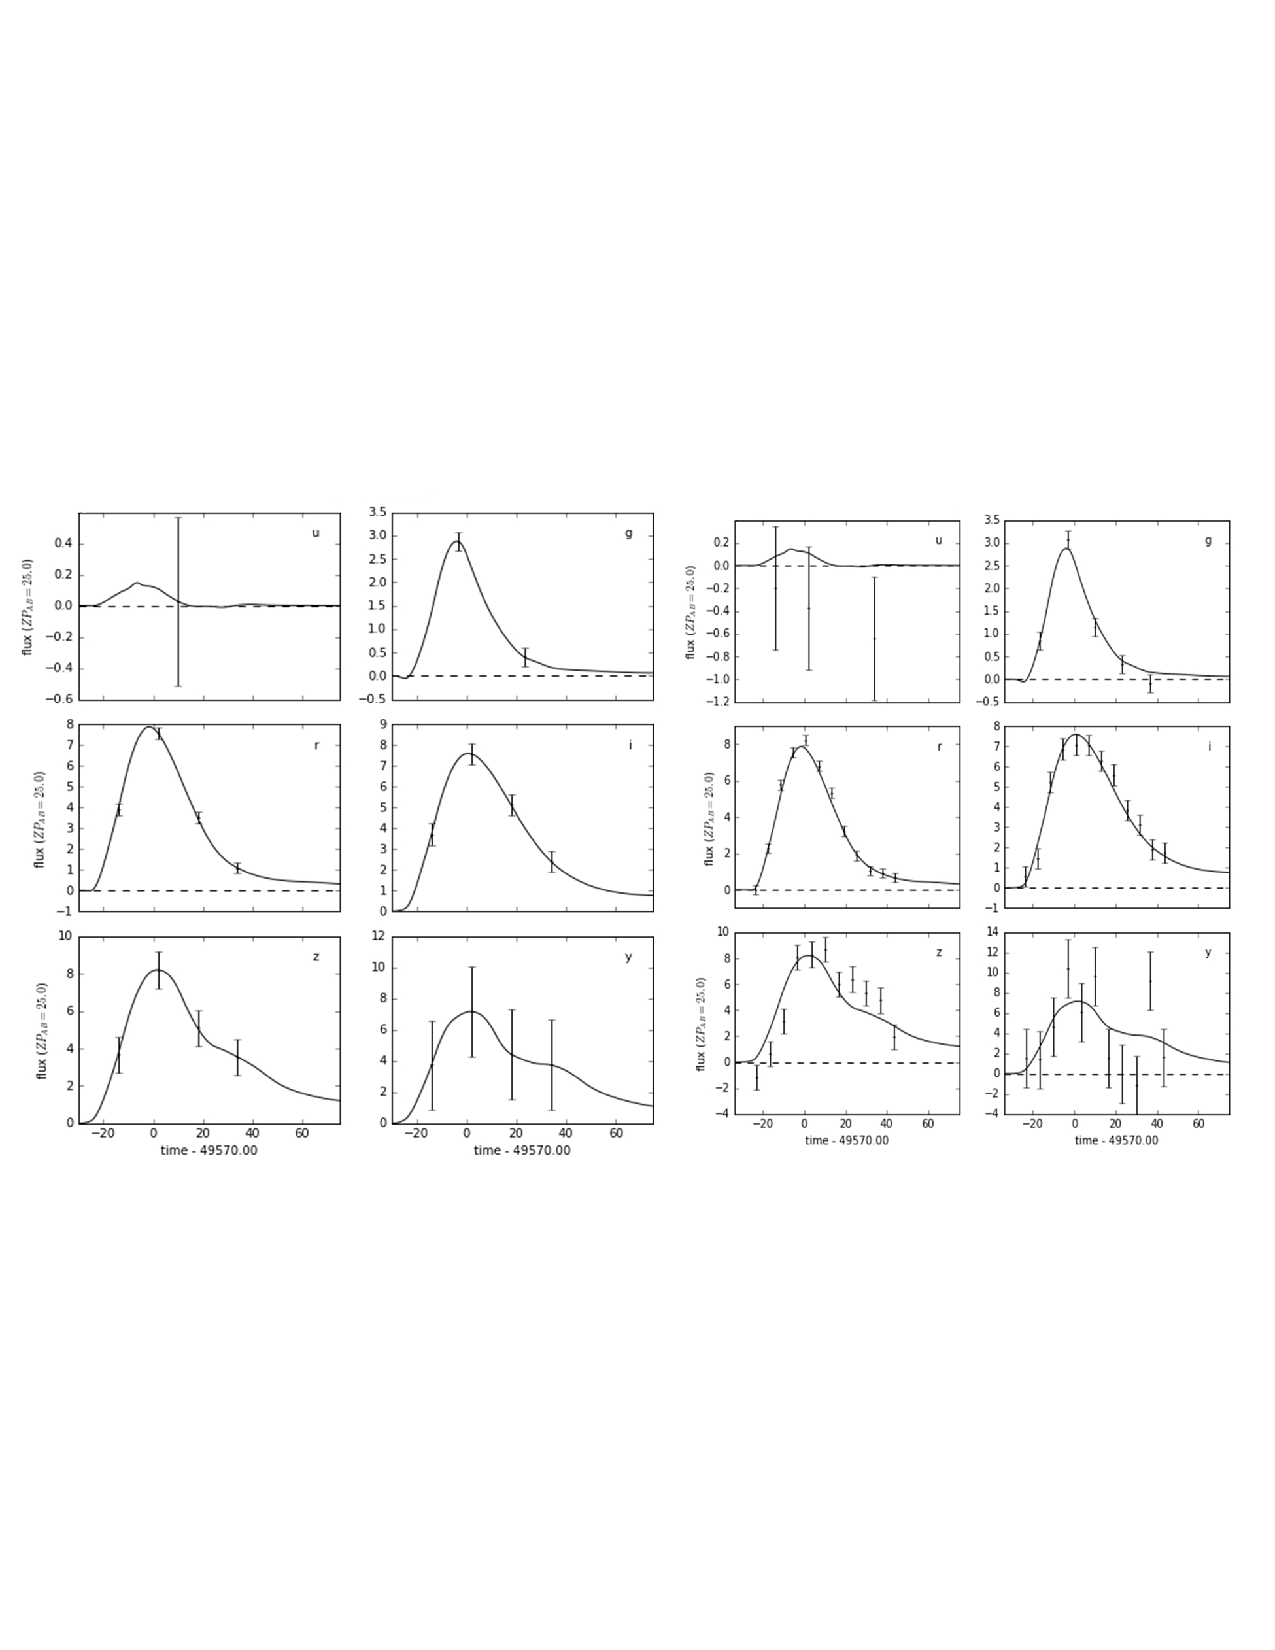
\includegraphics[width=13truecm]{figs/supernova/LCrandomseed.pdf}
\caption{An example of light curve of SN Type Ia generated using OpSim output
at RA. of 58$^{\circ}$ and Decl. of -27$^{\circ}$ (left) and the same light curve
after the sampling rate is enhanced by a factor of 3 (right).}
  \label{fig:LCrandom}
\end{figure}

\subsubsection{Details of rolling cadence of WFD optimized for SN cosmology }
%Ideally, we would propose changing the filter every day, and trebling the
%average WFD cadence in these smaller fields. Our primary goal is to  achieve our goal of 7-9 points per light
There are likely many possible LSST observing strategies one could propose to achieve our
goal of increasing the sampling of light curves by a factor of three. We hope to investigate
multiple OpSim runs in the future with a variety of implementations of rolling cadence.
In this section, we show a plausible observing strategy
that can achieve a factor of 3 increase in sampling rate in order to obtain reasonable-quality SN light curves.


The observing strategy of WDF is defined (see Section 1.6.2 in the LSST science book) as follows.

\noindent $\bullet$ A revisit time of three days on average per 10,000 deg$^2$ of sky (i.e., the area visible at any given time of the year), with two visits per night (particularly useful for establishing proper motion vectors for fast moving asteroids).

We define the 10,000 deg$^2$ survey area (the visible sky for a given time of the
year) simply as the ``visible sky".
In order to increase the sampling rate by a factor of 3, we propose to make the revisit time of $\sim$1 day (1/3 of three days above)
on average visible
sky. This means one third of the visible sky ($\sim$3300 deg$^2$) can be chosen. Preference
may be given to the part of
sky with low air-mass, but at the same time
a uniform coverage of LSST needs to be considered.
Ideally we would propose a filter change every day, and observe approximately the same
patch of visible sky for
$\sim$ 50 days before
going to another part.
As a result,
 the light curves will have  a sampling rate ($\times$3) in time.
A total of 1.4$\times$10$^5$ SNe Ia (Section 11.2.2 in \citet{2009arXiv0912.0201L}) expected from
WDF would become a factor of 2-3 lower
(details are to be investigated in future), but
the SNe that LSST WFD discovered will have  meaningful, reasonable-quality light curves which can be used to
classify the types of SNe and to improve cosmological parameters.

\subsection{Conclusion}

Here we answer the ten questions posed in Sub-section 1.2.1:

\begin{description}
\item[Q1:] {\it Does the science case place any constraints on the
tradeoff between the sky coverage and coadded depth? For example, should
the sky coverage be maximized (to $\sim$30,000 deg$^2$, as e.g., in
Pan-STARRS) or the number of detected galaxies (the current baseline but
with 18,000 deg$^2$)?}

\item[A1:] For supernova observations, the most important aspect is cadence: we need a
good sampling of well-measured light curves of supernovae. If the sky
coverage can be increased without sacrificing the number of observations
per supernova (i.e., over one season), such as using a rolling cadence
strategy, this will greatly improve supernova science. Inasmuch as
requiring increased sky coverage could negatively affect cadence over one
season, our preference is not to increase to a larger sky coverage.

\item[Q2:] {\it Does the science case place any constraints on the
tradeoff between uniformity of sampling and frequency of  sampling? For
example, a rolling cadence can provide enhanced sample rates over a part
of the survey or the entire survey for a designated time at the cost of
reduced sample rate the rest of the time (while maintaining the nominal
total visit counts).}


\item[A2:] Frequency of sampling is much more important than uniformity over long time
scales for all forms of supernova science. For SN Ia cosmology, light-curve
sampling should be about three times as frequent as for the current
baseline WFD cadence. While further investigation is needed, a reasonable
length of a season with enhanced rates is around 120-150 days. A rolling
cadence will allow this improved sampling while still keeping the sky
coverage and co-added depth, by concentrating on different fields in
different seasons (see Section 9.5 for details).

\item[Q3:] {\it Does the science case place any constraints on the
tradeoff between the single-visit depth and the number of visits
(especially in the $u$-band where longer exposures would minimize the
impact of the readout noise)?}

\item[A3:] In general for supernova science, the number of visits is more important to
the single-visit depth, though we would not advocate any decrease in
single-visit exposure time (below 2x15 sec). The U band  is useful for the
low-z (wide-area) sample and and their calibration of the Hubble diagram.
It is not obvious if longer exposures are helpful at this time for
supernova science.

\item[Q4:] {\it Does the science case place any constraints on the
Galactic plane coverage (spatial coverage, temporal sampling, visits per
band)?}

\item[A4:] Our supernova science is extragalactic and will use high Galactic-latitude
fields almost exclusively (to minimize Milky Way extinction systematic
uncertainties). Survey time spent on Galactic fields takes away from survey
time for our science; we would optimize for less time in the Galactic
plane.

\item[Q5:] {\it Does the science case place any constraints on the
fraction of observing time allocated to each band?}


\item[A5:] For supernova science, we have no strong preference for any band and would
benefit from roughly uniform depth per band. While redder bands are more
useful for higher redshift supernovae, the bluer bands are helpful
especially for lower redshift objects. Visits in each band should be
uniformly spread in time. A higher number of visits to redder bands is
preferred for DDF.

\item[Q6:] {\it Does the science case place any constraints on the
cadence for deep drilling fields?}


\item[A6:] Our optimal cadence would for the DDFs would be nightly or every other
night; every three nights would be acceptable. Beyond this we run the risk
of large gaps more than $\sim$7 days, which would be detrimental to supernova
science. Ideally, the DDFs would be observed in all available filters,
though not all filters are needed every night (so for instance some filters
could be observed on night 1, the others on night 2, and repeat). The
single-night depth should be 1-2 mag deeper than a WFD field, but not much
more; any extra time is better spent on a different night.

We would like a suitable number of extragalactic DDFs in total so that at
least a few ($\sim$3 to 5) are being observed at any time in the survey: we
would limit an increase in the number of DDFs if it came at the expense of
our preferred high cadence. Each field should be observed for a $``$season" of
length at least $\sim$120-150 days, staggering the fields so new fields cycle in
as old ones cycle out. In addition, for DDFs, the u-band exposure time
could be increased to minimize readout noise.

\item[Q7:] {\it Assuming two visits per night, would the science case
benefit if they are obtained in the same band or not?}



\item[A7:]Supernova science benefits enormously from having color information,
particularly in discovery and early epochs to help classification. Two
visits in the same band will be less useful than visits in different bands.

\item[Q8:] {\it Will the case science benefit from a special cadence
prescription during commissioning or early in the survey, such as:
acquiring a full 10-year count of visits for a small area (either in all
the bands or in a  selected set); a greatly enhanced cadence for a small
area?}



\item[A8:] During commissioning, we would like as many DDFs as possible observed in
all filters (with few times the per-night exposure time) so that templates
can be created for each of the DD fields we consider. This will allow us to
find useful supernovae in these DDFs as soon as the survey starts, and
provide us with useful time to deal with any issues in the image
subtraction etc. before the survey begins.

Early in the survey, we must build templates for all fields (more broadly
than just the DDFs). Our favored method for doing this is to devote the
bulk of year 1 to covering the full sky area, with a rolling cadence survey
commencing thereafter. As above, the templates should be at least a few
times the exposure time of a single visit (so that the template noise does
not dominate the subtraction). This is particularly important in the first
3-5 weeks of the survey, to ensure that we get useful data from the rest of
the critical first year.

\item[Q9:] {\it Does the science case place any constraints on the
sampling of observing conditions (e.g., seeing, dark sky, airmass),
possibly as a function of band, etc.?}


\item[A9:] While supernova observations benefit from good seeing, it is not as strong
a requirement as it is for other science cases. Moreover we would like to limit
any image coaddition issues for very good seeing (under the assumption that
these remain): we can make good use of observing conditions with slightly
poorer seeing.


\item[Q10:] {\it Does the case have science drivers that would require
real-time exposure time optimization to obtain nearly constant
single-visit limiting depth?}

\item[A10:]A sufficiently long (or nominal), fixed exposure time should be adequate
for supernova science. No real-time optimization is necessary, and
single-visit science is not the limiting factor for SNe science.


\end{description}



% \subsection{Rolling Cadence of the Main Survey Optimized for Supernova Science}
%
% \subsubsection{ Scientific Motivation for Rolling-Cadence}
%
% The main survey is important for the discovery of supernovae (SNe) in
% the redshift range of 0.1- 1, which is critical to constraint SN
% cosmological parameters. In order to identify a variable source as a SN
% and to distinguish the source as a Type Ia SN, we need 7-10 epochs
% spread over 45 days or so for each filter based on past experience.
% Universal survey of the Baseline Cadence provides 6 filter data for
% approximately 18 days (assuming a survey with a filter can be done for 3
% days). This provides 15 data points over 45 days and 2.5 data points in
% average for each filter. Our analysis of OpSim run (Baseline Observing
% Strategy) output shows the light curves of SNe from the OpSim data are
% insufficient not only to identify the source as a SN and but also to
% classify the SN if the SN is type Ia or II (or Ib, Ic). Our proposed
% observing strategy is critical to improve the quality of SN light
% curves. The light curves will have at least 3 times densely populated
% data points in time.
%
%
% \subsubsection{Proposed Rolling-Cadence of the Main Survey Optimized for SN Science }
%\label{sec:\secname:discussion}

% {\it Discussion: what risks have been identified? What suggestions could be
% made to improve this science project's figure of merit, and mitigate
% the identified risks?}
%
% Our goal for observing strategy optimized for SN cosmology is to
% obtain 7-10 epochs spread over 50 days or so for more than one filter. We suggest to
% change the filter every day and LSST can choose a part of sky which has the best airmass,
% centered on Zenith. LSST will observe about 1/3 of visible sky per day (to be confirmed).
% LSST can observe the same part of sky for 6 days with 6 filters, and repeat 9 times for
% the same field. This observing strategy will result in 54 visits (with 6 different
% filters) for the same field. We repeat the same for Field 2 which takes another 54 days.
% Then observe Field 3 for another 54 days.
%
% We propose a new Observing Strategy of the main survey (the Universal Cadence area;
% WFD) in order to generate 3 times densely populated SN light curves in time (i.e. 3
% times higher samples for a SN light curve). Our main goal is to obtain 7-10 epochs
% spread over 45 days per filter. For simplicity, we assume the main survey will cover
% available sky (2293 fields) for 3 days (we divide the available sky into 3 separate
% Sectors, which would be called Sector 1 and 2 and 3. Each Sector of the sky
% corresponds to ~764 fields. The sum of Sector 1 and 2 and 3 is 2293 fields, a total
% number of LSST fields from the Universal Cadence area. For a day, 1/3 of available
% sky would be observed. By changing the filter, every day, it will take 6 days to
% observe 6 filters for 1/3 of available sky. We repeat 9 times for the same Sector of
% sky, which will result in 54 visits (with 6 different filters) for the same Sector
% (1/3 of available sky). We repeat the same for the 2nd Sector of sky which takes
% another 54 days. Then we observe the 3rd Sector for another 54 days.
%
% To visualize this idea, we list our proposed observing strategy day by day; Day 1 :
% Filter 1 (for the 1st Sector), Day 2: Filter 2 (for the 1st Sector), Day 3: Filter 3
% (for the 1st Sector), Day 4: Filter 4 (for the 1st Sector), Day 5: Filter 5 (for the
% 1st Sector), and Day 6: Filter 6 (for the 1st Sector). Repeat this sequence 9 times
% for the 1st Sector. This will generate 54 data points for 54 days for a supernova and
% 9 data points in average for each filter. This is approximately 3 times higher sample
% of data for 54 days than those from the Universal Cadence. Observe the same sequences
% for the 2nd Sector (it takes 54 days) and then do the same for the 3rd Sector of sky
% (it takes another 54 days). This summarizes overall idea, but since visible sky is
% slightly different every day and observation depends on the weather, an OpSim run is
% needed accounting for all of these factors (and maybe other factors that we haven't
% mentioned here). One may also consider to observe each Sector for 108 days (2x54
% days) instead of 54 days; this may allow us to discover a higher number of SNe in
% stead of for 54 days. Our suggestion is mainly for the sky of Galactic latitude
% greater than 30 degree (|l| > 30) since it would be hard to discover SNe at the
% Galactic plane.
%
% \subsubsection{Expectations}
%
% \begin{enumerate}
% \item SN light curves would have 3 times more densely populated in time as we have designed.
% \item An average airmass of the Main Survey would be significantly lower.
% \item Significantly higher number of SN discovery can be expected because its impact area is
% large. The average number of visits per filter for 50 days is only $\sim$2 for the regions
% located from Dec. -65 to Dec. 0 based on Baseline Observing Strategy, but the number would
% be $\sim$6 with our proposed rolling cadence.
% \end{enumerate}



% %\begin{figure}[tbh!]
% \begin{figure}
% \vskip 3truecm
% %\vskip -1.3in
% %\includegraphics[angle=0,width=0.99\hsize:,clip]{figs/SNIaLCopsim.pdf}
% %\vskip -1.3in
% \caption{Predicted light curves of Supernova Type Ia using
% Rolling-Cadence. We used ramdom generation of time sequence (TO BE
% INCLUDED).}
% \label{fig:SNIaLCopsimmainnew}
% \end{figure}



% \begin{itemize}
% \item Intrinsic Dispersion, environmental effects, newer analysis methods
% \item Follow-up
% procedures: What is feasible? Where will our training samples for classification and light
% curve models come from (other experiments, our own sub-samples with spectroscopic
% follow-up?), spectroscopic follow-up of host galaxies. Can hosts be identified?
% \item `Systematics': In what ways will the real data not match the assumptions made in analysis.
% Having a large sample of SN, to understand the astrophysics would be useful for this.
% \end{itemize}


% ====================================================================

\navigationbar

%\end{document}


% --------------------------------------------------------------------

% ====================================================================
%+
% SECTION NAME:
%    lenstimedelays.tex
%
% CHAPTER:
%    cosmology.tex
%
% ELEVATOR PITCH:
%    Lensed quasars and supernovae provide distance measurements for
%    cosmology. They are a few days to a few weeks in length. To
%    measure them well we need long campaigns (>~3 years) with high
%    night-to-night cadence (better than the standard 5 days if
%    possible, especially as combining all filters might be difficult.)
%
% AUTHORS:
%   Phil Marshall (@drphilmarshall)
%-
% ====================================================================

\section{ Strong Gravitational Lens Time Delays }
\def\secname{lenstimedelays}\label{sec:\secname}

\credit{drphilmarshall},
\credit{rhiannonlynne},
\credit{tanguita}

The multiple images of strongly lensed quasars and supernovae have
delayed arrival times: variability in the first image will be observed
in the second image some time later, as the photons take different
paths around the deflector galaxy, and through different depths of
gravitational potential. If the lens mass distribution can be modeled
independently, using a combination of high resolution imaging of the
distorted quasar/SN host galaxy and stellar dynamics in the lens
galaxy, the measured time delays can be used to infer the ``time delay
distance'' in the system. This distance enables a direct physical measurement
of the Hubble constant, independent of the distance ladder.  \citet{TM16} provide a recent review of this cosmological probe, including its the main systematic errors and observational follow-up demands. High resolution follow-up imaging and spectroscopy is needed to constrain the lens galaxy mass distribution, and this is expected to dominate the systematic error budget in systems with good measured time delays. In tis section we investigate the cadence needed for LSST to provide these good time delays, in lensed quasar systems. We leave the assessment of lensed supernova time delays to future work.

% --------------------------------------------------------------------

\subsection{Target measurements and discoveries}
\label{sec:\secname:targets}

For this cosmological probe to be competitive with LSST's others, the
time delays of several hundred systems (which will be distributed
uniformly over the extragalactic sky) will need to be measured with
bias below the sub-percent level, while the precision required is a
few percent per lens.  In galaxy-scale lenses, the kind that are most
accurately modeled, these time delays are typically between several
days and several weeks long, and so are measurable in monitoring
campaigns having night-to-night cadence of between one and a few days,
and seasons lasting several months or more.

This size of sample seems plausible: \citet{OM10} predicted that several thousand lensed quasar systems should be detectable at LSST single visit depth and resolution, and \citet{LiaoEtal2015} found that around 400 of these should yield time delay measurements of high enough quality for cosmography.
To obtain accurate as well as precise lensed quasar time delays, several
monitoring seasons are required. Lensed supernova time delays have not
yet been measured, but their transient nature means that their time
delay measurements may be more sensitive to cadence than season or
campaign length.

% --------------------------------------------------------------------

\subsection{Metrics}
\label{sec:\secname:metrics}

Anticipating that the time delay accuracy would depend on night-to-night
cadence, season length, and campaign length, we carried out a large
scale simulation and measurement program that coarsely sampled these
schedule properties. In \citet{LiaoEtal2015}, we simulated 5 different
light curve datasets, each containing 1000 lenses, and presented them to
the strong lensing community in a ``Time Delay Challenge.'' These 5
challenge ``rungs'' differed by their schedule properties, in the ways
shown in \autoref{tab:tdcrungs}. Entries to the challenge consisted of samples of measured time delays, the quality of which the challenge team then measured via three primary diagnostic metrics: time delay accuracy, time delay
precision, and useable sample fraction (\ie the number of lenses that could be measured well, divided by the number of simulated lenses in the dataset). The accuracy of a sample was defined to be the mean fractional offset between the estimated and true time delays within the sample. The precision of a sample was defined to be the mean reported fractional uncertainty within the sample.


Focusing on the best challenge
submissions made by the community, we derived a simple power law model
for the variation of each of the time delay accuracy, time delay
precision, and useable sample fraction, with the schedule properties
cadence, season length and campaign length. These models are shown in
\autoref{fig:tdcresults}, reproduced from \citet{LiaoEtal2015}, and are
given by the following equations:
\begin{align}
|A|_{\rm model} &\approx 0.06\% \left(\frac{\rm cad} {\rm 3 days}  \right)^{0.0}
                          \left(\frac{\rm sea}  {\rm 4 months}\right)^{-1.0}
                          \left(\frac{\rm camp}{\rm 5 years} \right)^{-1.1} \notag \\
  P_{\rm model} &\approx 4.0\% \left(\frac{\rm cad} {\rm 3 days}  \right)^{ 0.7}
                         \left(\frac{\rm sea}  {\rm 4 months}\right)^{-0.3}
                         \left(\frac{\rm camp}{\rm 5 years} \right)^{-0.6} \notag \\
  f_{\rm model} &\approx 30\% \left(\frac{\rm cad} {\rm 3 days}  \right)^{-0.4}
                        \left(\frac{\rm sea}  {\rm 4 months}\right)^{ 0.8}
                        \left(\frac{\rm camp}{\rm 5 years} \right)^{-0.2} \notag
\end{align}

%%%%%%%%%%%%%%%%%%%%%%%%%%%%%%%%%%%%
\begin{table*}
\begin{center}
\capstart
\begin{tabular}{cccccc} \hline\hline
  Rung &  Mean Cadence & Cadence Dispersion & Season   & Campaign & Length   \\
       &  (days)       & (days)             & (months) & (years)  & (epochs) \\ \hline
  0    &    3.0        &   1.0              &   8.0    &    5     & 400      \\
  1    &    3.0        &   1.0              &   4.0    &    10    & 400      \\
  2    &    3.0        &   0.0              &   4.0    &    5     & 200      \\
  3    &    3.0        &   1.0              &   4.0    &    5     & 200      \\
  4    &    6.0        &   1.0              &   4.0    &    10    & 200      \\
\hline\hline
\end{tabular}
\end{center}
\caption{The observing parameters for the five rungs of the Time Delay
Challenge. Reproduced from \citet{LiaoEtal2015}.\label{tab:tdcrungs}}
\end{table*}
%%%%%%%%%%%%%%%%%%%%%%%%%%%%%%%%%%%%

%%%%%%%%%%%%%%%%%%%%%%%%%%%%%%%%%%%
\begin{figure*}[!ht]
  \capstart
  \begin{minipage}[b]{\linewidth}
    \begin{minipage}[b]{0.48\linewidth}
      \centering\includegraphics[width=\linewidth]{figs/Precision_cadence_nca.pdf}
    \end{minipage} \hfill
    \begin{minipage}[b]{0.48\linewidth}
      \centering\includegraphics[width=\linewidth]{figs/Fraction_season_nca.pdf}
    \end{minipage}
  \end{minipage}
\caption{Examples of changes in precision $P$
(left) and success fraction $f$ (right) with schedule properties, as
seen in the different TDC submissions. The gray approximate power law
model was derived by visual inspection of the pyCS-SPL results; the
signs of the indices were pre-determined according to our expectations.
Reproduced from \citet{LiaoEtal2015}.}
\label{fig:tdcresults}
\end{figure*}
%%%%%%%%%%%%%%%%%%%%%%%%%%%%%%%%%%%

All three of these diagnostic metrics would, in an ideal world, be
optimized: this could be achieved by decreasing the night-to-night
cadence (to better sample the light curves), extending the observing
season length (to maximize the chances of capturing a strong variation
and its echo), and extending the campaign length (to increase the number
of effective time delay measurements).

The quantity of greatest scientific interest is the {\it accuracy in
cosmological parameters}: this could be computed as follows. Setting a
required accuracy threshold  defines the available number of lenses,
which in turns gives us the mean precision per lens there. Combining the
whole sample, we would get the error on the weighted mean time delay, as
used by \citet{Coe+Moustakas2009}. This uncertainty, which scales as one
over the square root of the number of available lenses,  can be roughly
equated to the statistical uncertainty on the Hubble constant \citep{Coe+Moustakas2009,TM16}. The
Figure of Merit would be the final percentage precision on $H_0$, as a
way to sum up the sample size and time delay measurability (at fixed
accuracy requirement).

% --------------------------------------------------------------------

\subsection{\OpSim Analysis}
\label{sec:\secname:analysis}

% \OpSim analysis: how good would the default observing strategy be, at
% the time of writing for this science project?

In this section we present the results of our ongoing \OpSim / MAF
analysis, as we start to try to
answer the question ``how good would the proposed observing
strategies be, for time delay lens cosmography?''

\autoref{fig:lenstimedelays:accuracymaps} shows maps of TDC2 time delay
measurement accuracy from our MAF analysis of two \OpSim databases, the
baseline cadence \opsimdbref{db:baseCadence}, and a ``No Visit Pairs''
strategy, \opsimdbref{db:NoVisitPairs}. We use the \metric{TdcMetric} to compare three different
analysis scenarios, differing by a) whether or not we can combine all 6
filters' light curves such that they behave like the TDC2 single-filter
simulations (as was assumed by \citeauthor{LiaoEtal2015}), and b)
whether we wait 5 or 10 years before making the time delay measurement.\footnote{Here, ``years'' means ``seasons:'' we used the
\metric{SeasonStacker} to work
with seasons, rather than calendar years.}

These sky maps saturate at a threshold of 0.04\%, chosen conservatively
to be 5 times stricter than that used by
\citeauthor{Hojjati+Linder2014}. We can see that the area of sky
providing lenses measurable at this accuracy or better increases
markedly as we move from $ri$ to $ugrizy$. These maps predict that while
the accuracy should increase between DR5 and DR10, the sky area yielding
accuracy better than 0.04\% should already be close to the full WFD area
(18000 square degrees) by DR5: this bodes well for our ability to make
use of shorter campaign sky areas observed at higher frequency, as would
emerge from a rolling cadence strategy.

To summarize the diagnostic metric results, we first compute the area of
this ``high accuracy'' ($A < 0.04\%$) sky. We can then compute the cadence, season, and
campaign length just in these areas; these values are reported in
\autoref{tab:lenstimedelays:results}. The high accuracy area can be used
to define a ``Gold Sample'' of lenses, whose mean precision per lens we
can compute. The TDC2 useable fraction averaged over this area gives us
the approximate size of this sample: we simply re-scale the 400 lenses
predicted by \citet{LiaoEtal2015} by this fraction over the 30\% found
in TDC2. While these numbers are approximate, the ratios between
different observing and analysis strategies provide a useful indication of relative merit. In this table, the impacts of higher night-to-night sampling rate and survey length can be seen.\footnote{The small decrease in the number of useable lenses with $ugrizy$ going from 5 years to 10 years is due to the slightly lower precision in 5 years, and is an artifact of how the metrics are calculated (as global means rather than running totals).}


As described above, we follow \citet{Coe+Moustakas2009} and compute a
very simple time delay distance Figure of Merit ``\texttt{DPrecision}''
as follows. We first combine the fractional time delay precision in
quadrature with an assumed 4\% ``modeling uncertainty,'' and then divide
this by the square root of the number of Gold Sample lenses. This
estimated ensemble distance precision can be straightforwardly related
to cosmological parameter precision, as \citet{Coe+Moustakas2009} show
(it's very roughly the precision on the Hubble constant).  This distance
precision Figure of Merit is given in the final column of
\autoref{tab:lenstimedelays:results}. We see that in DR5, being able to
combine all filters instead of just $ri$ should give a FoM of 0.29\%
instead of 1.25\%; between DR5 and DR10 this then should improve to
0.24. This suggests that time delay measurement is primarily {\it
analysis-limited}. In the ``No Visit Pairs'' strategy, we seet that the
DR5 all-band FoM is 0.26\%, just a 10\% improvement. This might be
because the ``No Visit Pairs'' does not {\it insist} that the visits in
the visit pairs are split over different nights, only that they don't
{\it have} to be taken on the same night. We might expect a more
aggressive approach to splitting visit pairs to make a bigger difference --
but it seems unlikely that it would be a factor of two improvement.

%%%%%%%%%%%%%%%%%%%%%%%%%%%%%%%%%%%
\begin{figure*}[!ht]
  \capstart
  \begin{minipage}[b]{\linewidth}
    \begin{minipage}[b]{0.48\linewidth}
       \centering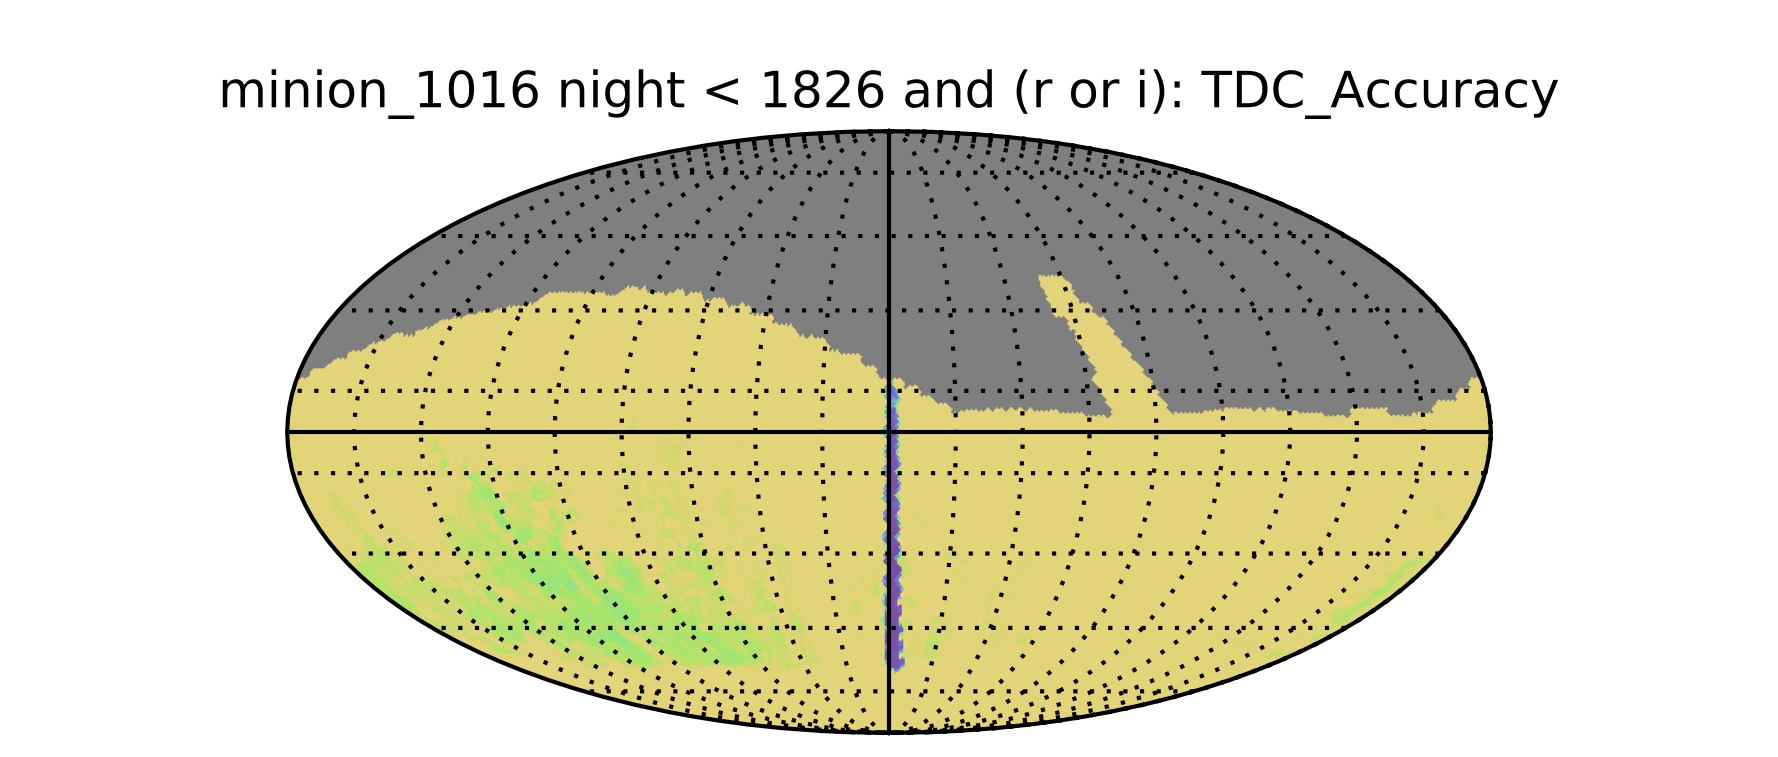
\includegraphics[width=\linewidth]{figs/lenstimedelays/minion_1016_TDC_Accuracy_night_lt_1826_and_r_or_i_HEAL_SkyMap.png}
    \end{minipage} \hfill
    \begin{minipage}[b]{0.48\linewidth}
       \centering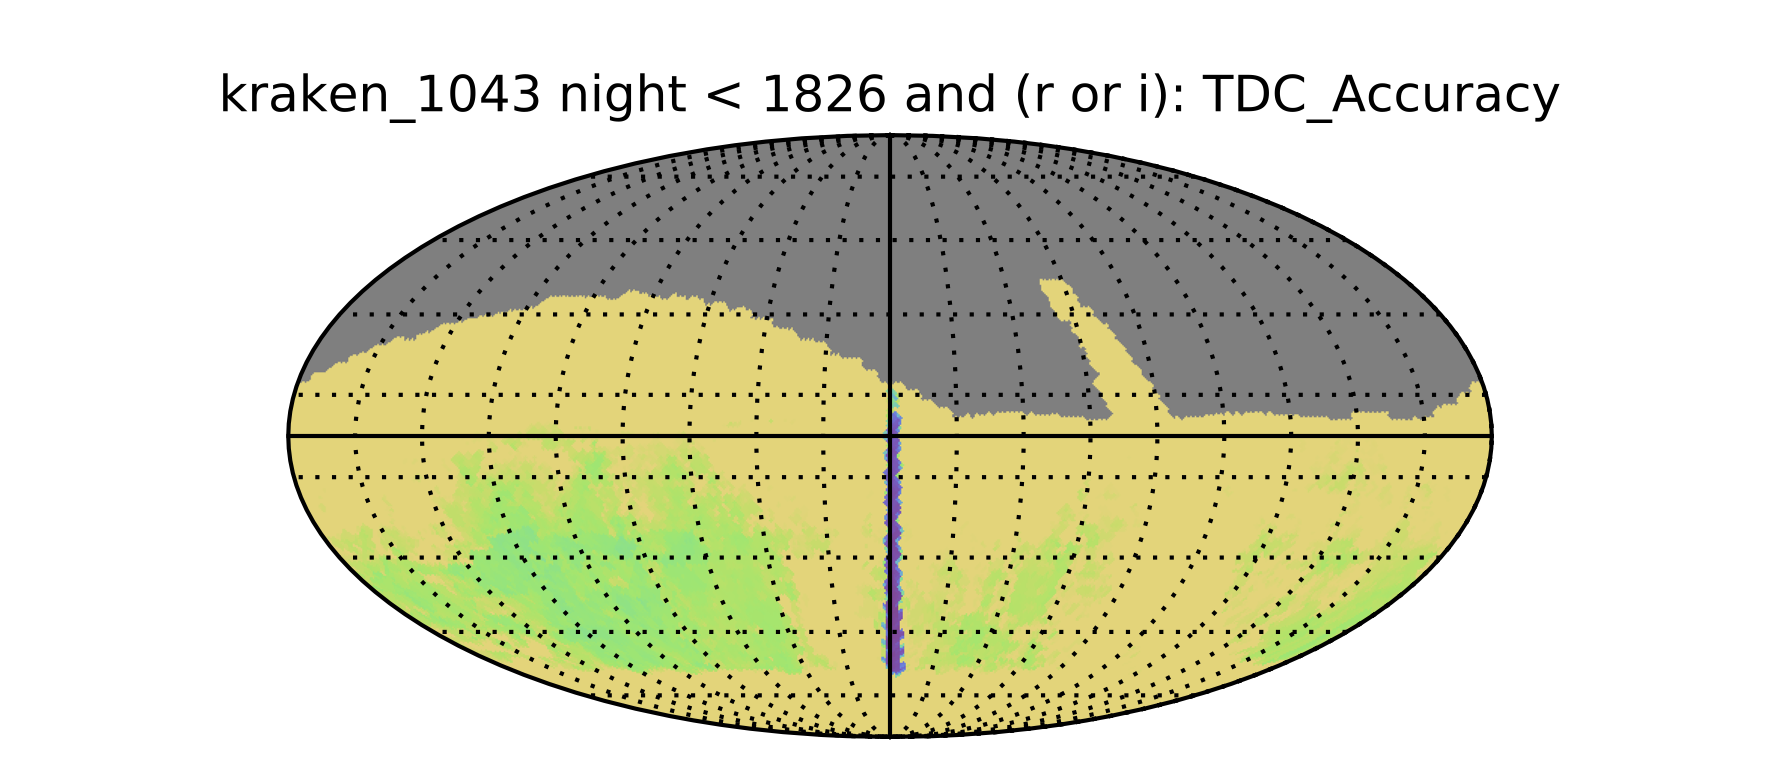
\includegraphics[width=\linewidth]{figs/lenstimedelays/kraken_1043_TDC_Accuracy_night_lt_1826_and_r_or_i_HEAL_SkyMap.png}
    \end{minipage}
  \end{minipage}
  \begin{minipage}[b]{\linewidth}
    \begin{minipage}[b]{0.48\linewidth}
       \centering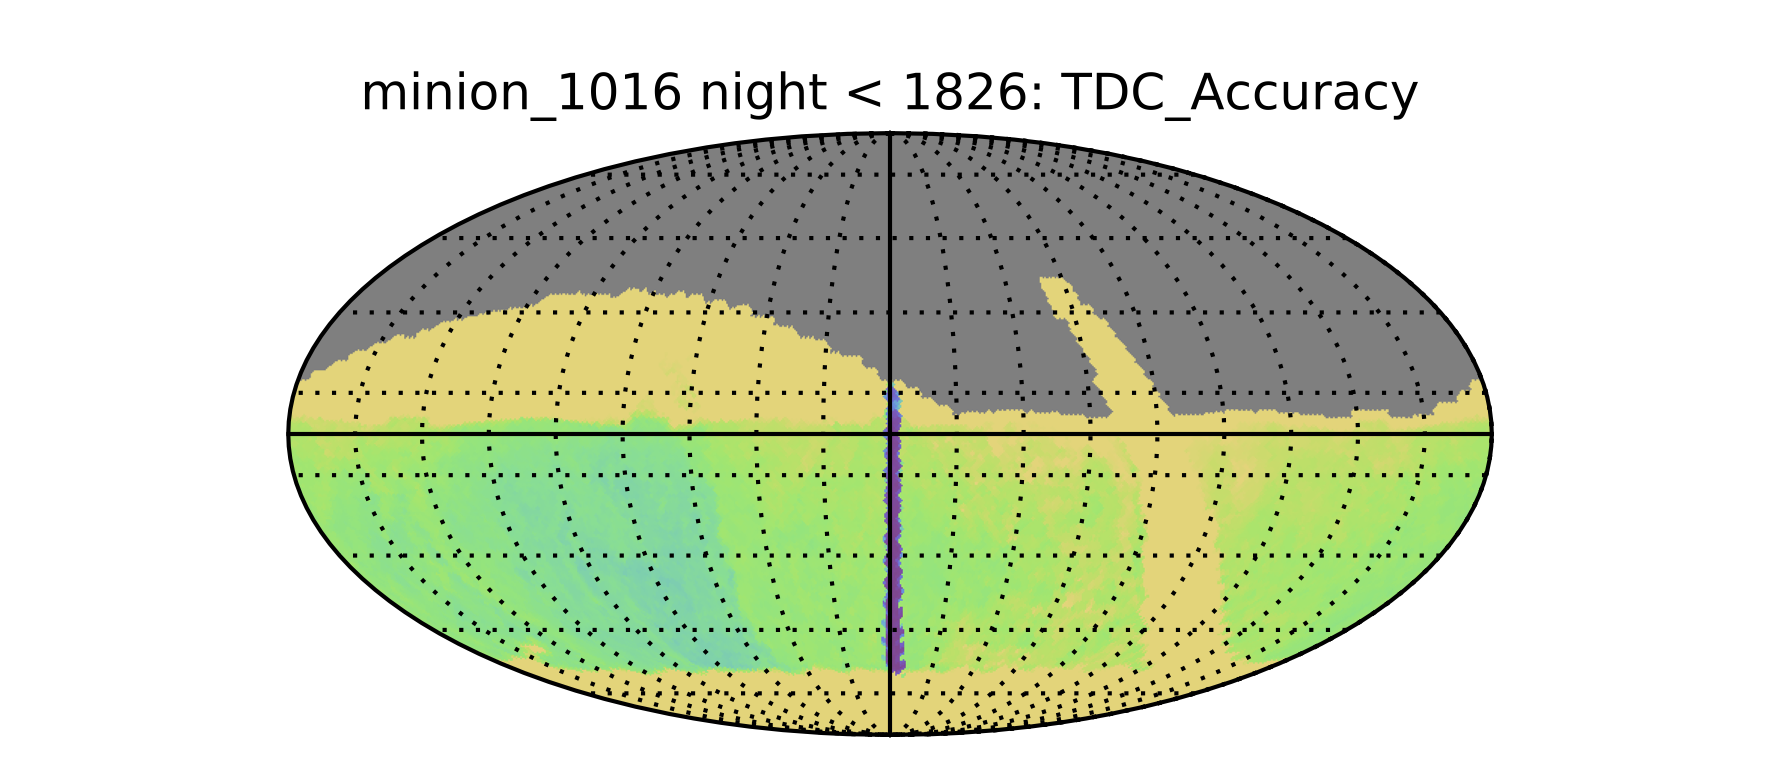
\includegraphics[width=\linewidth]{figs/lenstimedelays/minion_1016_TDC_Accuracy_night_lt_1826_HEAL_SkyMap.png}
    \end{minipage} \hfill
    \begin{minipage}[b]{0.48\linewidth}
       \centering\includegraphics[width=\linewidth]{figs/lenstimedelays/kraken_1043_TDC_Accuracy_night_lt_1826_HEAL_SkyMap.png}
    \end{minipage}
  \end{minipage}
  \begin{minipage}[b]{\linewidth}
    \begin{minipage}[b]{0.48\linewidth}
       \centering\includegraphics[width=\linewidth]{figs/lenstimedelays/minion_1016_TDC_Accuracy_night_lt_3652_HEAL_SkyMap.png}
    \end{minipage} \hfill
    \begin{minipage}[b]{0.48\linewidth}
       \centering\includegraphics[width=\linewidth]{figs/lenstimedelays/kraken_1043_TDC_Accuracy_night_lt_3652_HEAL_SkyMap.png}
    \end{minipage}
  \end{minipage}
\caption{Sky maps of the TDC2 time delay measurement accuracy metric $A$ for the baseline cadence \opsimdbref{db:baseCadence} (left) and the ``No Visit Pairs'' strategy, \opsimdbref{db:NoVisitPairs} (right). The rows show the build up of data quality with time and analysis capability, from 5 years of $r$ and $i$-band light curve data only (top row), to 5 years of hypothetically-combined $ugrizy$ light curve data (middle row), to 10 years of hypothetically-combined $ugrizy$ light curve data (bottom row). The maps saturate at the threshold accuracy of 0.04, such that any regions that are {\it not yellow} should yield high accuracy lens time delays, while the yellow regions show where high accuracy time delay measurement is not possible.}
\label{fig:lenstimedelays:accuracymaps}
\end{figure*}
%%%%%%%%%%%%%%%%%%%%%%%%%%%%%%%%%%%

%%%%%%%%%%%%%%%%%%%%%%%%%%%%%%%%%%%%%%

\begin{table*}
\begin{center}
\caption{Lens Time Delay Metric Analysis Results.}
\label{tab:lenstimedelays:results}
\footnotesize
\begin{tabularx}{\linewidth}{ccccccccc}
  \hline
  \OpSim run                       % runName -> db
   & Filters                       % filters
    & Years                        % Nyears
     & \texttt{cadence}            % high_accuracy_cadence
      & \texttt{season}            % high_accuracy_season
       & \texttt{Area}             % high_accuracy_area
        & \texttt{dtPrecision}     % precision_per_lens
         & \texttt{Nlenses}        % N_lenses
          & \texttt{DPrecision} \\ % distance_precision
  \hline\hline
  \opsimdbref{db:baseCadence}
   & $ugrizy$
    & $10$
     & $4.5$
      & $6.9$
       & $19004$
        & $5.09$
         & $468$
          & $0.24$ \\
  \opsimdbref{db:baseCadence}
   & $ugrizy$
    & $5$
     & $5.1$
      & $6.6$
       & $17926$
        & $6.29$
         & $472$
          & $0.29$ \\
  \opsimdbref{db:baseCadence}
   & $ri$
    & $10$
     & $10.4$
      & $5.7$
       & $18566$
        & $7.07$
         & $285$
          & $0.42$ \\
  \opsimdbref{db:baseCadence}
   & $ri$
    & $5$
     & $14.2$
      & $5.5$
       & $4841$
        & $10.81$
         & $75$
          & $1.25$ \\
  \opsimdbref{db:NoVisitPairs}
   & $ugrizy$
    & $10$
     & $3.9$
      & $7.1$
       & $18907$
        & $4.88$
         & $502$
          & $0.22$ \\
  \opsimdbref{db:NoVisitPairs}
   & $ugrizy$
    & $5$
     & $4.5$
      & $6.7$
       & $18093$
        & $5.93$
         & $504$
          & $0.26$ \\
  \opsimdbref{db:NoVisitPairs}
   & $ri$
    & $10$
     & $8.5$
      & $6.1$
       & $18617$
        & $6.34$
         & $329$
          & $0.35$ \\
  \opsimdbref{db:NoVisitPairs}
   & $ri$
    & $5$
     & $10.7$
      & $6.1$
       & $9358$
        & $9.35$
         & $171$
          & $0.71$ \\
   \hline

\multicolumn{9}{p{\linewidth}}{\scriptsize Notes: see the text for
the definitions of each metric.}
\end{tabularx}
\normalsize
\medskip\\
\end{center}
\end{table*}
%%%%%%%%%%%%%%%%%%%%%%%%%%%%%%%%%%%%%%


% --------------------------------------------------------------------

\subsection{Discussion}
\label{sec:\secname:discussion}

The main risk involved with this science case is that the
``multi-filter'' light curve analysis presented here, which extrapolates
from the results of the single-filter TDC1, does not represent
accurately the real-life combination of all 6 filters together. The
second time delay challenge (TDC2) will help answer this question.  For
now, just using 2 filters gives an upper limit on the overall precision
we should expect.

Naively, we would expect the relaxation of the visit pairs requirement
to increase the  night-to-night cadence by a factor of two, if the
visits are redistributed randomly in time. However, it seems \OpSim is
not as liberal as this, such that we do not see much improvement over
the baseline cadence. Efficiency maximization could be preventing visits
being fully split. We are interested in any changes to the WFD survey
time sampling that reduce the inter-night gaps: these  would include
rolling cadence schemes.


% ====================================================================

\subsection{Conclusions}

Based on the above results, we now answer the ten questions posed in
\autoref{sec:intro:evaluation:caseConclusions}:

\begin{description}

\item[Q1:] {\it Does the science case place any constraints on the
tradeoff between the sky coverage and coadded depth? For example, should
the sky coverage be maximized (to $\sim$30,000 deg$^2$, as e.g., in
Pan-STARRS) or the number of detected galaxies (the current baseline
of 18,000 deg$^2$)?}

\item[A1:] Yes: it's probably better to have smaller area and better
data, especially if the multi-filter light curve analysis turns out to
be difficult. This conclusion is partly informed by the apparently small
difference between 5 years and 10 years campaign length, although we
need to be careful: COSMOGRAIL studies show that the longer monitoring
campaigns yield significantly higher accuracy results.

\item[Q2:] {\it Does the science case place any constraints on the
tradeoff between uniformity of sampling and frequency of sampling? For
example, a rolling cadence can provide enhanced sample rates over a part
of the survey or the entire survey for a designated time at the cost of
reduced sample rate the rest of the time (while maintaining the nominal
total visit counts).}

\item[A2:] Yes: higher frequency is better, up to the point where the
visit separation becomes less than one night. We would like to see the
additional visits gained through rolling cadence used to fill in the
nights in the campaign rather than going deeper by taking more visits
per night.

\item[Q3:] {\it Does the science case place any constraints on the
tradeoff between the single-visit depth and the number of visits
(especially in the $u$-band where longer exposures would minimize the
impact of the readout noise)?}

\item[A3:] Yes: we have not investigated this in detail, but it's very
likely that we'd prefer more shallow visits than fewer deeper visits.

\item[Q4:] {\it Does the science case place any constraints on the
Galactic plane coverage (spatial coverage, temporal sampling, visits per
band)?}

\item[A4:] No: only inasmuch as that time spent in the plane could have
been used to improve the night-to-night sampling frequency. The effect
is probably not large.

\item[Q5:] {\it Does the science case place any constraints on the
fraction of observing time allocated to each band?}

\item[A5:] Yes, but: in principle an all $i$-band survey would make time
delay estimation easier. However, since we need the other filters to
assist with lens finding and lens environment characterization, we'd be
reluctant to advocate any move away from the universal $ugrizy$
coverage.

\item[Q6:] {\it Does the science case place any constraints on the
cadence for deep drilling fields?}

\item[A6:] To first order, no.

\item[Q7:] {\it Assuming two visits per night, would the science case
benefit if they are obtained in the same band or not?}

\item[A7:] Unclear: different bands are probably going to be
better, but this has not been tested. It would clearly provide good
information on the AGN color variability model.

\item[Q8:] {\it Will the case science benefit from a special cadence
prescription during commissioning or early in the survey, such as:
acquiring a full 10-year count of visits for a small area (either in all
the bands or in a  selected set); a greatly enhanced cadence for a small
area?}

\item[A8:] Not really. We rely on the difference imaging working well,
so making a good template across as much sky as possible would be good.
Including a known lens system (from DES, perhaps) in any deep field
would be useful too: we would be happy if the cadence to be similar to
WDF to be able to test our software.

\item[Q9:] {\it Does the science case place any constraints on the
sampling of observing conditions (e.g., seeing, dark sky, airmass),
possibly as a function of band, etc.?}

\item[A9:] No.

\item[Q10:] {\it Does the case have science drivers that would require
real-time exposure time optimization to obtain nearly constant
single-visit limiting depth?}

\item[A10:] No.

\end{description}

\navigationbar

% ====================================================================


% --------------------------------------------------------------------
